%%%%%%%%%%%%%%%%%%%%%%%%%%%%%%%%%%%%%%%%%%%%%%%%%%%%%%%%%%
% Determining the document class and the input encoding: %
%%%%%%%%%%%%%%%%%%%%%%%%%%%%%%%%%%%%%%%%%%%%%%%%%%%%%%%%%%

\documentclass[paper=a4, fontsize=10.5pt, parskip=false, oneside, pointlessnumbers, leqno]{scrartcl}

\newcommand{\eqnum}{\leavevmode\hfill\refstepcounter{equation}\textup{\tagform@{\theequation}}}
% \documentclass[paper=a4, fontsize=11pt, twoside]{scrartcl}
% \documentclass[a4paper,twoside,11pt,fleqn]{article}
% \usepackage{typearea}
\typearea[2.5mm]{8}
\setlength{\textheight}{22.1cm}
% \setlength{\textwidth}{12cm}
\usepackage{lscape}

\DeclareFontFamily{OT1}{pzc}{}
\DeclareFontShape{OT1}{pzc}{m}{it}{<-> s * [1.10] pzcmi7t}{}
\DeclareMathAlphabet{\mathpzc}{OT1}{pzc}{m}{it}

\newcommand\smallO{
  \mathchoice
    {{\scriptstyle\mathcal{O}}}% \displaystyle
    {{\scriptstyle\mathcal{O}}}% \textstyle
    {{\scriptscriptstyle\mathcal{O}}}% \scriptstyle
    {\scalebox{.7}{$\scriptscriptstyle\mathcal{O}$}}%\scriptscriptstyle
  }

\usepackage{bbm}
\newtheorem{proposition}{Proposition}[section]
%\newtheorem{proof}[proposition]{Proof}
\newtheorem{proposition and definition}[proposition]{Proposition and Definition}
\newtheorem{definition}[proposition]{Definition}
\newtheorem{lemma}[proposition]{Lemma}
\newtheorem{theorem}[proposition]{Theorem}
%\newtheorem{example}[proposition]{Example}
\newtheorem{corollary}[proposition]{Corollary}
\newtheorem{remarks}[proposition]{Remarks}
\newtheorem{remark}[proposition]{Remark}
\newtheorem{assumptions}[proposition]{Assumption}
\newcommand{\timesim}{\raisebox{-2.2mm}{
\unitlength 1.00pt
\linethickness{0.5pt}
\begin{picture}(10.00,20.00)
\multiput(2.00,6.00)(0.12,0.18){50}{\line(0,1){0.18}}
\multiput(2.00,15.00)(0.12,-0.18){50}{\line(0,-1){0.18}}
\put(5.00,2.00){\makebox(0,0)[cc]{$\scriptstyle i=1$}}
\put(5.00,18.00){\makebox(0,0)[cc]{$\scriptstyle r$}}
\end{picture}
}}

\usepackage{subcaption}
% \usepackage[ansinew]{inputenc}
% \usepackage[applemac]{inputenc}
% This package enables you to input special characters---like umlauts---
% via hitting the corresponding keys on your keyboard, instead of
% having to use LaTeX commands like \"{a}, \"{o} etc.

%\usepackage{mathtools}
%\mathtoolsset{showonlyrefs=true}

%\usepackage{autonum}

%%%%%%%%%%%%%%%%%%%%%%%%%%%%%%%%%%%%%%%%%%%%%%%%%%%%%%%%
% Commands influencing the page design and typography: %
%%%%%%%%%%%%%%%%%%%%%%%%%%%%%%%%%%%%%%%%%%%%%%%%%%%%%%%%

\usepackage[USenglish, ngerman]{babel}

\usepackage{fixltx2e}

% Provides the ``\textsubscript'' command

\usepackage{ragged2e}

% Provides, among others, the \RaggedRight environment, which is \raggedright but with hyphenation enabled.

% Typeset the title, authors' names, and affiliations ragged right

\makeatletter
\def\maketitle{%
  % \null
  % \thispagestyle{empty}%
  % \vfill
  \linespread{1.05}
  \renewcommand{\thefootnote}{\fnsymbol{footnote}}
  \begin{RaggedRight}
    \leavevmode
    {\normalfont \LARGE \@title \par}%
    \vskip 20pt
    {\sffamily \bfseries \normalsize \@author \par}%
    \vskip 20pt
    {\sffamily \normalsize \@date \par}%
    \vskip 7.5pt
  \end{RaggedRight}%
  {\@thanks}
  % \vfill
  % \null
  % \cleardoublepage
  \setcounter{footnote}{0}
  }
\makeatother

\usepackage[bottom, splitrule]{footmisc}
\setlength{\footnotemargin}{0.97\parindent}
\let\oldfootnoterule\footnoterule
\renewcommand{\footnoterule}{\bigskip\oldfootnoterule\smallskip}
% Replace the asterisk in the footnotes marked with symbols by a star:
\DefineFNsymbols*{stars}{{$\star$}\dagger\ddagger\S\P\|%
                   {$\star\star$}{\dagger\dagger}{\ddagger\ddagger}}
\setfnsymbol{stars}

\let \footnoteorig \footnote
\renewcommand{\footnote}[1]{\footnoteorig{\:#1}}

% Setting up the fonts to use (needs the respective packages to be installed!):
% Just delete the percent sign "%" in front of the package combination that you want to use and
% insert a percent sign in front of the packages that you don't use:

\usepackage[flushleft, online, para]{threeparttable}
% Provides the `table notes' environment

\usepackage{amsmath, amssymb}
% This package makes additional mathematical commands and symbols available. For example, standard LaTeX
% knows a command "\begin{eqnarray} ... \end{eqnarray}" for typesetting a sequence of equations. However,
% it numbers each of the equations involved - which you might not want. Therefore, the package "amsmath"
% provides the command "\begin{eqnarray*} ... \end{eqnarray*}" which suppresses the numbering.
% \usepackage{amssymb}

\renewcommand{\dots}{\ldots{\kern -1pt}}

% \usepackage[charter, sfscaled=false]{mathdesign}
% \renewcommand{\rmdefault}{bch}
% \usepackage{charter}

\usepackage{fourier}
\DeclareMathAlphabet{\mathbfit}{T1}{fut\mathfamilyextension}{bx}{it}
\newcommand{\gammaup}{\othergamma}

%\usepackage{txfonts}
%\usepackage[LY1]{fontenc}

\newcommand{\euro}{\texteuro}

%\DeclareSymbolFont{rmcustom}{T1}\rmdefault\mddefault\updefault
%\DeclareMathSymbol{(}{\mathopen}{rmcustom}{`(}
%\DeclareMathSymbol{)}{\mathclose}{rmcustom}{`)}
%\DeclareMathSymbol{[}{\mathopen}{rmcustom}{`[}
%\DeclareMathSymbol{]}{\mathclose}{rmcustom}{`]}
%\DeclareMathDelimiter{\lbrace}{\mathopen}{rmcustom}{`\{}{largesymbols}{"08}
%\DeclareMathDelimiter{\rbrace}{\mathclose}{rmcustom}{`\}}{largesymbols}{"09}
%\DeclareMathDelimiter{\leftcurly}{\mathopen}{rmcustom}{`\{}{largesymbols}{"08}
%\DeclareMathDelimiter{\rightcurly}{\mathclose}{rmcustom}{`\}}{largesymbols}{"09}
%\renewcommand{\{}{\leftcurly}
%\renewcommand{\}}{\rightcurly}
% \DeclareMathAlphabet{\mathbfit}{T1}{chr}{bx}{it}
% \usepackage[defaultsans, scale=0.87]{opensans}
\usepackage[scaled=0.92]{helvet}
\usepackage[scaled=0.84]{beramono}
% \usepackage[defaultsans]{droidsans}
% \usepackage[defaultmono, scale=0.865]{droidmono}
% \usepackage[scaled=0.93]{PTSans}
% \usepackage{PTSansNarrow}

\usepackage{textcomp}

% sets the font of text and formulae to Utopia; sets the sans-serif and monospaced font to Bera
% \usepackage{mathptmx} \usepackage[scaled=0.9]{helvet} \usepackage{courier}
% sets the font of text and formulae to Times; sets the sans-serif font to Helvetica;
% sets the monospaced font to Courier
% \usepackage[charter]{mathdesign} \usepackage{berasans} \usepackage{beramono}
% \usepackage{charter}
% \DeclareSymbolFont{rmcustom}{T1}\rmdefault\mddefault\updefault
% \DeclareMathSymbol{(}{\mathopen}{rmcustom}{`(}
% \DeclareMathSymbol{)}{\mathclose}{rmcustom}{`)}
% \DeclareMathSymbol{[}{\mathopen}{rmcustom}{`[}
% \DeclareMathSymbol{]}{\mathclose}{rmcustom}{`]}
% \DeclareMathDelimiter{\leftcurly}{\mathopen}{rmcustom}{`\{}{largesymbols}{"08}
% \DeclareMathDelimiter{\rightcurly}{\mathclose}{rmcustom}{`\}}{largesymbols}{"09}
%\renewcommand{\{}{\leftcurly}
%\renewcommand{\}}{\rightcurly}
% sets the font of text and formulae to ITC Charter; sets the sans-serif and monospaced font to Bera
% \usepackage[osf]{mathpazo} \usepackage[scaled=0.9]{helvet} \usepackage{courier}
% sets the font of text and formulae to Palatino; sets the sans-serif font to Helvetica;
% sets the monospaced font to Courier

\frenchspacing
% By default LaTeX inserts an enlarged space after every period (.). Since the period (.) creates
% much white space anyway, enlarging the subsequent space is unnecessary. The \frenchspacing command
% suppresses the insertion of additional white space.

\flushbottom  % forces the bottom text lines on each page to be horizontally aligned

\sloppy  % less punishment for large whitespace within text lines

% \usepackage[activate]{pdfcprot}
% \usepackage[protrusion=true, factor=1200, expansion=compatibility]{microtype}
\usepackage[protrusion=true, expansion=false, kerning=true]{microtype}
% This package enables so-called hanging punctuation. That is, when a punctuation sign like ":", ".", "-" etc.
% is found at the beginning or end of a line, it is protruded a little into the page margin. This leads to
% so-called "optical margin alignment", because the protrusion makes the margin alignment look straighter.
\SetExtraKerning[unit=space]
  {encoding={*}, family={*}, series={*}, size={*, footnote size}}
  {\textemdash={325,325}}

\usepackage{enumitem}
\setlist[enumerate]{leftmargin=\parindent, listparindent=\parindent, parsep=0pt, labelsep=0.42\parindent}

% \def\semismall{\@setfontsize{\semismall}{10.25pt}{13.5pt}}
\renewenvironment{quote}
                 {\list{}{\leftmargin\parindent \rightmargin\parindent}%
                  %\small
                  \setlength{\baselineskip}{2.8ex}\item\relax}
                 {\endlist}

\newenvironment{tightitemize}{
  \begin{list}{\makebox(5.5,4.5)[t]{$\scriptstyle \bullet$}}{%
    \advance\partopsep  by \topsep
    \setlength{\topsep}{0.75ex}
    \setlength{\itemsep}{0in}
    \setlength{\parsep}{0em}
    \setlength{\leftmargin}{\parindent}
    \setlength{\rightmargin}{0in}
    \setlength{\itemindent}{0in}
  }
}
{\end{list}}

\newcommand{\highlight}[1]{\textcolor{medred}{[[\:\textbf{#1}\:]]}}

% Packages to influence table layout:
\usepackage{tabularx}
% \usepackage{tabulary}
\usepackage{booktabs}
\heavyrulewidth=.05em
% \belowbottomsep=-2.5pt
\usepackage{multirow}
% Enables the "\multirow" command for typesetting cells inside tables which span several rows.
% \usepackage{colortbl}

% A package to change the formatting of the table of contents:
\usepackage[titles]{tocloft}
\setlength{\cftbeforesecskip}{1ex}
\renewcommand{\cftsecfont}{\sffamily\bfseries\selectfont}
\renewcommand{\cftsecpagefont}{\sffamily\bfseries\selectfont}
\cftsetrmarg{27.5pt}
\cftsetpnumwidth{22.5pt}
\makeatletter
  \renewcommand{\@tocrmarg}{27.5pt plus1fil}
\makeatother

% A package to change the formatting of the captions for tables and figures:
%\usepackage{caption}
%\DeclareCaptionLabelSeparator{colon}{:\ \ \ }
%\captionsetup{format=hang, labelsep=colon, justification=RaggedRight, font={sf, small}, labelfont=bf}
% Formatting the captions:
\usepackage{caption}
\captionsetup{
  figureposition=below,
  tableposition=above,
  format = plain,
  labelsep=period,
  margin = \parindent,
  font = {sf, footnotesize},
  labelfont = {bf},
  justification = centering
}
% \usepackage[margin=\parindent, justification=centering, font=small]{caption}[2007/04/16]

%% Disable single lines at the start of a paragraph (Schusterjungen)
%\clubpenalty = 10000
%% Disable single lines at the end of a paragraph (Hurenkinder)
%\widowpenalty = 10000 \displaywidowpenalty = 10000
\usepackage[all]{nowidow}

\renewcommand{\bottomfraction}{0.99}
\renewcommand{\topfraction}{0.99}

\linespread{1}

% \include{letterspacing}
% \newcommand{\caps}[1]{\scalebox{0.97}{\letterspace to 1.06\naturalwidth{#1}}}
\newcommand{\caps}[1]{\scalebox{0.97}{\textls[50]{#1}}}
\newcommand{\code}[1]{\texttt{#1}}
% \newcommand{\code}[1]{\scalebox{0.98}{\textls[5]{\texttt{#1}}}}
% The \textls command is only available if microtype has been loaded

\newcommand{\dbreak}{\hspace{0pt}}	% discretionary line break


%%%%%%%%%%%%%%%%%%%%%%%%%%%%%%%%%%%%%%%%
% Commands influencing the PDF output: %
%%%%%%%%%%%%%%%%%%%%%%%%%%%%%%%%%%%%%%%%

\usepackage[pdftex]{graphicx}
\usepackage[table]{xcolor}
\definecolor{UBonnBlue}{RGB}{000,066,145}
\definecolor{DarkWarmGrey}{RGB}{105,105,090}
\definecolor{WarmGrey}{RGB}{139,138,125}
\definecolor{darkblue}{rgb}{0.00,0.00,0.50}
\definecolor{medred}{rgb}{0.75,0.00,0.00}
\definecolor{darkred}{rgb}{0.70,0.00,0.00}
\definecolor{customgreen}{rgb}{0.2,0.6,0.00}
\usepackage[pdftex, pdftitle={Cognitive Load Increases Risk Aversion},
pdfauthor={Holger Gerhardt, Guido Biele, Harald Uhlig, Hauke~R. Heekeren}, pdfsubject={}, bookmarks=true, bookmarksopen=true,
bookmarksnumbered=true, bookmarksopenlevel=2, colorlinks=true, pdfpagemode=UseOutlines, pdfview=Fit,
pdfstartview=Fit, pdffitwindow=false, linkcolor=UBonnBlue, citecolor=UBonnBlue,%
% backref=page,
urlcolor=UBonnBlue]{hyperref}
\urlstyle{same}   % Sets URLs in the text font instead of the typewriter font
% \renewcommand{\url}[1]{\href{#1}{#1}}
% \usepackage{memhfixc}
% Only needed when using the "memoir" class

% Enclose the back references in the bibliography to the pages on which a reference is cited
% in square brackets (Econometrica style)
% \let \backrefold \backref
% \renewcommand*{\backref}[1]{[\backrefold{#1}]}

% Influencing the color and font sizes of the headings:
\addtokomafont{sectioning}{\color{UBonnBlue}}
% \addtokomafont{sectioning}{\color{darkred}}
% \addtokomafont{sectioning}{\rmfamily}
% \addtokomafont{section}{\fontseries{l}\selectfont\large} % for OpenSans only
% \addtokomafont{subsection}{\fontseries{sb}\selectfont\normalsize} % for OpenSans only
\addtokomafont{section}{\large}
\addtokomafont{subsection}{\normalsize} % for OpenSans only
% \addtokomafont{subsubsection}{\normalsize \mdseries}
% \addtokomafont{subsubsection}{\normalsize \rmfamily}

% For AEA.cls:
%\renewcommand{\subsubsection}[1]{%
%\addtocounter{subsubsection}{1}%
%\bigskip\textit{\arabic{subsubsection}.~#1}---}

% For scrartcl.cls:
\renewcommand{\subsubsection}[1]{%
\addtocounter{subsubsection}{1}%
\bigskip\noindent\emph{\hspace{\parindent}\arabic{subsubsection}.~#1}---\hspace{0pt}}
\newcommand{\runinhead}[1]{%
\bigskip\noindent\emph{\hspace{\parindent}#1.}---\hspace{0pt}}

% Hanging/constant-width section numbers:
\makeatletter
\def\@seccntformat#1{%
       \protect%
       \hspace{-31pt}%
       \makebox[31pt][l]{%
              \csname  the#1\endcsname%
              %\quad
              }%
   }
\makeatother


%%%%%%%%%%%%%%%%
% Commenting commands %
%%%%%%%%%%%%%%%%


\setlength{\marginparwidth}{4.1cm}
\setlength{\marginparsep}{0.4cm}
\setlength{\marginparpush}{0.4cm}
%\newcommand{\comment}[2]{\setbox99=\hbox{\textbf{\v{|}}}\textcolor{darkred}{\hspace{-0.75pt}\textbf{\raisebox{1.5pt}{\v{}}\hspace{-\wd99}\raisebox{0.5pt}{|}}}\hspace{0.75pt}\hspace{-\wd99}\marginpar{\RaggedRight \sffamily \footnotesize \setlength{\baselineskip}{2.35ex} \textcolor{darkred}{\textbf{#1}\\ #2}}}

\newcommand{\comment}[2]{\setbox99=\hbox{\textbf{\v{ }}}\makebox[0pt][l]{\hspace{-1.35pt}\textcolor{darkred}{\textbf{\raisebox{1.75pt}{\v{ }}\hspace{-0.827\wd99}|}}}\marginpar{\RaggedRight \sffamily%
%\fontseries{l}\selectfont
\footnotesize \setlength{\baselineskip}{2.35ex} \textcolor{darkred}{\textbf{%
%\fontseries{sb}\selectfont
#1}\\ #2}}}
% \renewcommand{\comment}[2]{}{}

\newcommand{\commentgreen}[2]{\setbox99=\hbox{\textbf{\v{ }}}\makebox[0pt][l]{\hspace{-1.35pt}\textcolor{customgreen}{\textbf{\raisebox{1.75pt}{\v{ }}\hspace{-0.827\wd99}|}}}\marginpar{\RaggedRight \sffamily%
%\fontseries{l}\selectfont
\footnotesize \setlength{\baselineskip}{2.35ex} \textcolor{customgreen}{\textbf{%
%\fontseries{sb}\selectfont
#1}\\ #2}}}
% \renewcommand{\commentgreen}[2]{}{}

%%%%%%%%%%%%%%%%%%%%%%%%%%%%%%%%%%%%
% Some user-defined math commands: %
%%%%%%%%%%%%%%%%%%%%%%%%%%%%%%%%%%%%

% The following line introduces a new command which makes it easy to typeset vectors and matrices,
% surrounded by regular (round) parentheses:
\newcommand{\rdmatrix}[1]{\left(\,\begin{matrix}#1\end{matrix}\,\right)}
% The same for vectors/matrices surrounded by square brackets:
\newcommand{\sqmatrix}[1]{\left[\,\begin{matrix}#1\end{matrix}\,\right]}
% Putting a backslash in front of "exp", "lim", "max" etc. makes LaTeX recognize the respective mathematical
% expression as a function or operator. These are then not set in italics but upright. It improves
% intellegibility of mathematical expressions to set the following operators upright, too:
%\newcommand{\E}{\mathrm{E}}
%\EE
\DeclareMathOperator{\bias}{Bias}
\DeclareMathOperator{\var}{Var}
\DeclareMathOperator{\tr}{tr}
\DeclareMathOperator{\supp}{supp}
\DeclareMathOperator{\cov}{Cov}


\newcommand{\equals}{\;=\;}
\newcommand{\mdash}{{\tiny{ }}---{\tiny{ }}}

\usepackage{commath}
%\usepackage{amsmath,amsfonts}
\DeclareMathOperator{\spn}{span}



\usepackage{rotating}

\usepackage{abstract}
\renewcommand{\absnamepos}{flushleft}
\renewcommand{\abstractnamefont}{\sffamily \bfseries \normalsize}

\usepackage{multicol}


%%%%%%%%%%%%%%%%%%%%%%%%%%%%%%%%%%%%%%%%%%%
% Commands connected to the bibliography: %
%%%%%%%%%%%%%%%%%%%%%%%%%%%%%%%%%%%%%%%%%%%

% The following package has to be loaded to be able to use the "Econometrica" bibliography style.
\usepackage{natbib}
% \usepackage[longnamesfirst]{natbib}
% \renewcommand{\harvardand}{and}
% \newcommand{\harvardand}{and}
% Since the "\cite" command puts parentheses around the cited work - which one doesn't want in most cases -
% it is useful to redefine the meaning of "\cite"
% \newcommand{\citep}[1]{(\citeauthor{#1}, \citeyear*{#1})}
% \newcommand{\cite}[1]{\citeauthor{#1}, \citeyear*{#1}}
% \renewcommand{\cite}[1]{\citeasnoun{#1}}


%%%%%%%%%%%%%%%%%%%%%%%%%%%%%%%
% Now the actual text begins: %
%%%%%%%%%%%%%%%%%%%%%%%%%%%%%%%

\usepackage{hyperref}
\hypersetup{pdfstartview={XYZ null null 0.88}}
\newcommand{\EE}{\mathop{\mbox{\sf E}}}
\newcommand{\quantnet}{\hspace*{\fill} \raisebox{-1pt}{\includegraphics[scale=0.05]{qletlogo}}\,}
%\hypersetup{linkcolor  = black}

\begin{document}

\selectlanguage{USenglish} \frenchspacing
% \pagenumbering{roman}
% Numbers the pages of the front matter by "i", "ii", "iii", "iv" and so on.

\begin{titlepage}

% \def\blfootnote{\xdef\@thefnmark{}\@footnotetext}

\title{Functional Principal Component Analysis \\for Derivatives of Multivariate Curves \thanks{$\:$Financial support from the German Research Foundation for the joint project no. 70102424 "Functional Principal Components for Derivatives and Higher Dimensions", between Humboldt-Universit\"at zu Berlin and Rheinische Friedrich-Wilhelms-Universit\"at Bonn, is gratefully acknowledged. We would like to thank as well the Collaborative Research Center 649 ``Economic Risk'' for providing the data and the International Research Training Group (IRTG) 1792 ``High-Dimensional Non-Stationary Time Series Analysis'', Humboldt-Universit�t zu Berlin for additional funding.}}



\author{Maria Grith,\textsuperscript{\!1}
Wolfgang K. H{\"a}rdle,\textsuperscript{\!1,2}
Alois Kneip \textsuperscript{\!3} and
Heiko Wagner\textsuperscript{\,3} \\[7.5pt]
\normalfont \scriptsize \sffamily
\textsuperscript{\phantom{0}1}\,Ladislaus von Bortkiewicz Chair of Statistics and C.A.S.E. - Center for Applied Statistics and Economics, School of Business and Economics, Humboldt-Universit\"at zu Berlin, Spandauer Stra{\ss}e 1, 10178 Berlin, Germany \\
\scriptsize \sffamily
\textsuperscript{\phantom{0}2}\,Sim Kee Boon Institute for Financial Economics, Singapore Management University, 81 Victoria Street, Singapore 188065 \\
\scriptsize \sffamily
\textsuperscript{\phantom{0}3}\,Institute for Financial Economics and Statistics, Department of Economics, Rheinische Friedrich-Wilhelms-Universit\"at Bonn, Adenauerallee 24-26, 53113 Bonn
}
\date{\vspace{-5ex}}
%\date{\medskip This version: \today}
\maketitle

\medskip

\setlength{\absleftindent}{0pt}
\setlength{\absrightindent}{0pt}
\setlength{\abstitleskip}{-\absparindent}
\setlength{\columnsep}{0.95pc}

\let\hyphenpenaltyorig=\hyphenpenalty
\let\toleranceorig=\tolerance
\begin{abstract}   \hyphenpenalty=10 \tolerance=500
\noindent We present two methods based on the functional principal component analysis (FPCA) for the estimation of smooth derivatives of a sample of functions observed in more than one-dimensional domain. We apply the eigendecomposition to a) the dual covariance matrix of the derivatives; b) the dual covariance matrix of the observed curves and take derivatives of their eigenfunctions. To handle noisy and discrete observations, we rely on the local polynomial regression. We show that if the curves are contained in a finite-dimensional function space, the second method performs better asymptotically. We apply our methodology in a simulation and real data study, to estimate state price density surfaces from call option prices. Using real data for the DAX 30 stock index between 2002 and 2011, we identify three components, which are interpreted as volatility, skewness and tail factors, and find evidence of term structure variation.
%We also find evidence for term structure variation.



%Our paper addresses the challenge of recovering the derivatives of high-dimension spatial noisy curves. We adapt the functional principal component analysis (FPCA) to the case of derivatives using the dual method and show how to estimate high-dimensional FPCA computationally efficient. We present two alternative methods to obtain the derivatives and compare their performance asymptotically and in finite sample. In a financial application that uses observed call option prices we estimate the state price density (SPD) surfaces and find that two components are sufficient to explain most of their variability. %and extract the economic content embedded in their dynamics.

%This allows us to reduce the model complexity and express curves variability in terms of few principal components and loadings that can be used for further analysis.

\medskip

\hyphenpenalty=\hyphenpenaltyorig \tolerance=\toleranceorig





\noindent \emph{Keywords:\:} functional principal component, dual method, derivatives, multivariate functions, state price densities

\medskip

\noindent \emph{JEL codes:\:} C13, C14, G13

\end{abstract}

\thispagestyle{empty}
% Suppresses the needless output of the page number on the title page.

\end{titlepage}

\pagenumbering{arabic}
% Sets the page numbering to the usual numbers: "1", "2", "3", "4" and so on.

\setcounter{page}{2}

\setlength{\baselineskip}{2.9ex}
\setlength{\parindent}{2.9ex}
% This influences the line spacing in the footnotes
%\linespread{1.075}
\linespread{1.5}

% \setlength{\mathindent}{\parindent}	% only if ``fleqn'' option is used

% Increases line spacing a bit, which improves legibility. This is especially useful for texts containing
% mathematical formulae, in order to prevent subscripts and superscripts in the formulae to collide with
% the following and previous lines, respectively.

\section{Introduction}

Over the last two decades functional data analysis became a popular tool to handle data entities that are random functions. Usually, discrete and noisy versions of them are observed. Oftentimes, these entities are multivariate functions, i.e., functions with more than one-dimensional domain. Examples include brain activity recordings generated during fMRI or EEG experiments (\cite{VanBommel2014}, \cite{majer:15}). %, environmental or climatological maps.
In a variety of applications though, the object of interest is not directly observable but can be recovered from the observed data by means of derivative. Typical examples of financial applications are functionals retrieved from the observed prices, such as implied risk neutral or state price density (\cite{Schienle:12}), pricing kernel (\cite{Gr:13}) or market price of risk (\cite{Lopez:12}). Motivated by such data analysis situations, we address the problem of estimating derivatives of multivariate functions from existing discrete and noisy data.
%high-dimensional spatial curves that are not empirically observable but can be recovered from the existing discrete and noisy data by means of derivatives. %An example of such an instance that motivates our present study are the SPDs implied by option prices. SPDs are continuous versions of Arrow Debreu prices that pay one unit of currency if one state is realized and zero otherwise. %Considered basic securities, they are not traded over exchanges but can be calculated from the prices of existing securities.

%The usefulness of knowing the shape and dynamics of SPDs derives, among others, from the possibility of fair pricing of exotic contingent claims because they are assumed to reflect equilibrium conditions on the market, see pricing under the risk neutral rule, e.g. \cite{Harrison:79}. Furthermore, due to the forward-looking perspective, they are used to estimate the physical density of the underlying asset by incorporating the adjustments for risks by means of pricing kernel, e.g. \cite{Anagnou:02}, \cite{Bliss:04}, \cite{Alonso:09}, \cite{Duca:14}. In addition, the exchanges calculate volatility indexes, such as VIX for S$\&$P 500 or VDAX for DAX 30, that reflect the market expected forward volatility. Also known by the investors as 'fear indices' they are computed from option prices, with a link to but not a straight forward interpretation of the implied densities.

%These adjustments require the understanding of behavioral risk patterns on the market - through the aggregate measures of preferences and beliefs - and this is possible by linking the implied state price to the physical densities, see \cite{hens:12}, \cite{Bakshi:10}, \cite{Polkovnichenko:12}, \cite{Kra:14}.
Functions, which are objects of an infinite-dimensional vector space, require specific methods that allow a good approximation of their variability with a small number of components. FPCA is a convenient tool to address this task because it allows us to explain complicated data structures with only a few orthogonal principal components that fulfill the optimal basis property in terms of its $L^2$ accuracy. These components are given by the Karhunen-Lo{\`e}ve theorem, see for instance \cite{Bosq:2000}. %In the one-dimensional case it is also easy to implement.
In addition, the corresponding principal loadings to this basis system can be used to study the variability of the observed phenomena. %, for example in a time series framework. In addition, depending on the application the corresponding principal scores can be interpreted, for example in a time series framework.
%The mathematical basis for the Karhunen-Lo{\`e}ve decomposition is given by the Hilbert-Schmidt theorem. % from the functional analysis theory. In the last years a lot of effort has been done to lay a theoretical foundation for the use of these insights in a statistical context.
An important contribution in the treatment of the finite-dimensional PCA was done by \cite{Pousse:82}, followed by subsequent studies that fostered the applicability of the method to samples of observed noisy curves. \cite{Besse:86}, among others, derived theoretical results for observations that are affected by additive errors. Some of the most important contributions for the extension of the PCA to functional data belong to \cite{cardot1999functional}, \cite{Cardot2007}, \cite{Vieu2006}, \cite{Mas2002117} and \cite{mas2008local}.
Simple, one-dimensional spatial curves are well understood from both numerical and theoretical perspectives and FPCA is easy to implement in this case. Multivariate objects, with more complicated spatial and temporal correlation structures, or not directly observable functions of these objects, such as derivatives, lack a sound theoretical framework. Furthermore, computational issues are considerable in higher-dimensional domain.

To our best knowledge, FPCA for derivatives has been tackled by \cite{Hall:09} and \cite{Mueller:2009}. The first study handles one-dimensional directional derivatives and gradients. The second paper analyses a particular setup in one-dimensional domain where the observations are sparse. This method is applicable to non-sparse data but can be computationally inefficient when dealing with large amounts of observations per curve. %There are no studies of derivatives using FPCA in more than one spatial dimension.
For the study of observed functions, there are a series of empirical studies for the two-dimensional domain case, see \cite{Cont:02} for an application close to our empirical study. Further proposals to implement FPCA in more than two dimensions to analyze functions, rather than their derivatives, have been done particularly in the area of brain imaging, see for instance, \cite{Zipunnikov:11} who implement multilevel FPCA (\cite{Staicu01042010}, \cite{di2009multilevel}) to analyze brain images of different groups of individuals. %apply multilevel FPCA (\cite{Staicu01042010}, \cite{di2009multilevel}) to analyze different groups of individuals. %For example, \cite{Zipunnikov:11} split the recorded data into smaller parts to make it manageable. This method, called multilevel FPCA (\cite{Staicu01042010}, \cite{di2009multilevel}), is well suited to analyze different groups of individuals.
However, a thorough derivation of statistical properties of the estimators is missing in these works.

%To our knowledge, the functional data analysis for derivatives has been done by \cite{Mueller:2009}, in a particular type of application in one-dimension where the observations are sparse. When applied to non-sparse data, the methodology is inefficient. Another paper by \cite{Hall:09} handles one-dimensional directional derivatives and gradients. There are no studies of derivatives using FPCA in more than one-dimension.

%Particularly when high-dimensional data is present, the computational aspect is not negligible. For every additional dimension exponentially many observations are needed to get the same rate of convergence. There is no straightforward way to generalize the commonly used procedures to compute the FPCA to the higher dimensional case, without getting into computational trouble. Complicated attempts has been done for example by \cite{Zipunnikov:11} where the data is split into smaller parts to be still calculable.

%A way to handle large amounts of observations was proposed by \cite{Benko:2009} where the duality relation is used for one-dimensional curves. Computational efficiency is essential with increasing spatial dimensions and the dual method performs better when the number of curves is smaller than the number of the discrete observations per curve. We will also use this approach here.

In this paper, we aim to fill in the existent gaps in the literature on FPCA for the study of derivatives of multivariate functions. We present two alternative approaches to estimate the derivatives. %and to apply the newly developed framework to the study of SPDs.
%The rest of the paper is organized as following: The theoretical framework, estimation procedure and statistical properties will be derived through sections \ref{t2} and \ref{t3} for general functions. Our empirical study in section \ref{t4} is guided by the estimation and dynamics analysis of option implied SPDs in a simulation study and real data example. Section \ref{t5} concludes.
These are not tailored to handle sparse data sets, as are other methods that aim to estimate the mean or covariance function of a sample of curves, see for instance \cite{cai2011} and \cite{zhang2016}. Furthermore, our approaches are feasible when the spatial dimension increases only under suitable smoothness assumptions of the underlying curves. Otherwise, the estimators that we propose suffer from the curse of dimensionality. %Our estimators suffer from increasing dimensions $g$ if no additional assumptions on the underlying data structure are made.


The paper is organized as follows: the theoretical framework, estimation procedure and statistical properties are derived through Section \ref{t2}. Our empirical study in Section \ref{t4} is guided by the estimation and the dynamics analysis of the option implied state price densities. It includes a simulation study and a real data example. %Section \ref{t5} concludes.


%\color{red}VIX = constructed by CBOE based on some continuous-time theory ??? Zhaogang 2013\color{black}

\section{Methodology}\label{t2}

%Handling infinite-dimensional data structures requires specific methods that allow the representation of their variability with a small number of components. Karhunen-Lo{\`e}ve decomposition is a convenient tool to address this task; it allows to explain complicated data structures with only a few principal components. In addition, the corresponding principal scores can be used to study the evolution of the observed phenomena, for example in a time series framework. %In addition, depending on the application the corresponding principal scores can be interpreted, for example in a time series framework.

%The mathematical basis for the Karhunen-Lo{\`e}ve decomposition is given by the Hilbert-Schmidt theorem. % from the functional analysis theory. In the last years a lot of effort has been done to lay a theoretical foundation for the use of these insights in a statistical context.
%An important contribution in this context has been done by \cite{Pousse:82}, followed by consequent studies that fostered the applicability of the method to samples of observed noisy curves. \cite{Benko:2009} and \cite{Besse:86}, among others, derived theoretical results for observations that are effected by additive errors.

%To date, simple, one-dimensional structures are well understood from both numerical and theoretical perspective. High-dimensional structures, with more complicated spatial and temporal correlation structures, or derivatives lack a sound theoretical framework. In addition, the computational issues are not negligible. A few papers have tackled the indirectly observed curves estimation. \cite{Hall:09} handle one-dimensional directional derivatives and gradients. \cite{Mueller:2009} analyze a particular setup in one-dimension where the observations are sparse. When applied to non-sparse data, this methodology is computationally inefficient. Though there are no studies of derivatives using FPCA in more than one-dimension. For the study on nonderivatives, there are a series of applied papers for the two-dimensional case, see \cite{Cont:02} for an application close to our empirical study. Complicated attempts to implement FPCA for nonderivatives in more that two dimensions has been done, for example by \cite{Zipunnikov:11}, where the data is split into smaller parts to make it manageable. However, a thorough derivation of the statistical properties of these estimators is missing.

%To our knowledge, the functional data analysis for derivatives has been done by \cite{Mueller:2009}, in a particular type of application in one-dimension where the observations are sparse. When applied to non-sparse data, the methodology is inefficient. Another paper by \cite{Hall:09} handles one-dimensional directional derivatives and gradients. There are no studies of derivatives using FPCA in more than one-dimension.

%Particularly when high-dimensional data is present, the computational aspect is not negligible. For every additional dimension exponentially many observations are needed to get the same rate of convergence. There is no straightforward way to generalize the commonly used procedures to compute the FPCA to the higher dimensional case, without getting into computational trouble. Complicated attempts has been done for example by \cite{Zipunnikov:11} where the data is split into smaller parts to be still calculable.

%A way to handle large amounts of observations with joint functional structure was proposed by \cite{Benko:2009} where the duality relation is used for one-dimensional curves. Computation efficiency is essential with increasing dimensions and the dual method performs better when the number of curves is smaller than the number of the discrete observations per curve. In this paper, we generalize this procedure to the case of derivatives in high-dimensions. Next, we will present two alternative methods to obtain the derivatives and in the subsequent two sections we will explain their comparative performance in terms of asymptotics and finite sample in a simulation study.


%In our empirical study we are guided by a finance application in which we want to explain the variability of option implied SPDs

% in which we want to explain the variability of option implied SPDs through dynamic parameters (principal scores) that can be interpreted within a time series framework.

%ADD STH ABOUT APPLICATION HERE!


%In this paper we aim to recover the derivatives of high-dimensional noisy curves, as well as to summarize them by few principal components and to explain their variability through dynamic parameters that can be interpreted within a time series framework. To achieve this goal we employ a functional data analysis (FDA) method based on the Karhunen-Lo{\`e}ve decomposition of a random curve via a set of orthonormal basis functions gained from the covariance operator. In particular, we will adapt the functional principal component analysis (FPCA) for curves to the case of their derivatives.

%The main assumption for performing this decomposition is that the curves are square integrable and their derivatives exist. One situation when this condition is fulfilled if the case of continuous phenomenon that can be represented as smooth functions. For a finite number of curves observed without errors the Karhunen-Lo{\`e}ve decomposition is applied to the sample counterpart of the covariance operator, as shown in \cite{Hall:2006}. If these curves are additionally observed at discrete points with noise, as it is often the case in practice, smoothing is required at some stage, see \cite{Benko:2009} or (reference Silverman for ex.) for additional details.

%Our approach is a generalization of the approach presented by \cite{Benko:2009}. They introduce a new method for the estimation of principal components of functions from discrete noisy data, based on the duality relation for matrices (see h�rlde book ref). One advantage of using this method is that no smoothing of individual curves is required to obtain an asymptotically unbiased estimator for the dual matrix of the covariance operator. Consequently, this estimation method doesn't suffer of the potential biases and inconsistencies introduced by smoothing involved in the application of other famous method e.g.(reference) to the noisy data. In addition, the method is computationally more efficient when the sample size is smaller than observation points (why, reference).

%To apply standard approaches which are based of decomposing the covariance directly, to higher dimensions has several problems: computational effort for computing the covariance matrix and the eigenvalues decomposition increases exponentially with every additional dimension. (why, reference) Besides, it is not clear how one can adapt the standard method to the high-dimensional case, in particular with respect to the derivation of theoretical properties of the estimators.

%To our knowledge, the functional data analysis for derivatives has only been done by \cite{Mueller:2009}, and only in a particular type of application with sparse data in one-dimension. (explain method) When applied to non-sparse data, the methodology is inefficient and causes not very good convergence rates (reference). There are no studies of derivatives using FPCA in more dimensions.

%(the advantage of analyzing all the curves together. estimating them using FPCA. signal to noise ratio, leveling down the noise by averaging, assumptions about the curves as being realizations from a stationary process)

%The paper is organized as follows:
%\subsection{Karhunen-Lo{\`e}ve decomposition and derivatives of (multivariate) functions}
\subsection{Two approaches to the derivatives of multivariate functions using FPCA}\label{fpca2}
%\subsection{Theoretical underpinnings}
%The representation of derivatives of multivariate curves requires a careful choice of notation.
In this section, we review FPCA from a technical point of view and make the reader familiar with our notation.

% $\EE\left[X(t)\right]=0$
Let $X$ be a centered smooth random function in $L^2([0,1]^g)$, where $g$ denotes the spatial dimension, with finite second moment $\int_{[0,1]^g} \EE\left[X(t)^2 \right]dt < \infty$ for $t=(t_1, \ldots, t_g)^{\top}$. %Here, we consider centered functions. %if non-centered curves are assume than there is a need to additionally subtract $E(Y)$.
The underlying dependence structure can  be characterized by the covariance function $\sigma(t,v)\stackrel{\operatorname{def}}{=}\EE\left[X(t)X(v)\right]$ and
 the corresponding covariance operator $\Gamma$% applied to some function $\vartheta \in L^2([0,1]^g)$
 \begin{equation*}
%\Gamma \vartheta(t)=\int_{[0,1]^g}\sigma(t,v)\vartheta(v)dv,
(\Gamma \vartheta)(t)=\int_{[0,1]^g}\sigma(t,v)\vartheta(v)dv.
\end{equation*}
%Under weak conditions $\Gamma$ is a Hilbert-Schmidt operator and possesses a countable number of non-negative eigenvalues.
Mercer's lemma guarantees the existence of a set of eigenvalues $\lambda_1\geq \lambda_2\geq \dots$ and a corresponding system of orthonormal eigenfunctions $\gamma_1,\gamma_2,\dots$ called functional principal components such that
\begin{equation} \label{op}
\sigma(t,v)= \sum_{r=1}^\infty \lambda_r \gamma_r(t) \gamma_r(v),
\end{equation}
where the eigenvalues and eigenfunctions satisfy
%\begin{equation*} \label{y}
$(\Gamma \gamma_r)(t)=\lambda_r\gamma_r(t)$. Moreover, $\sum_{r=1}^\infty \lambda_r=\int_{[0,1]^g}\sigma(t,t)dt$.
%\end{equation*}
%Let $\lambda_1\geq \lambda_2\geq \dots$ denote the ordered eigenvalues of $\sigma$ and let $\gamma_1,\gamma_2,\dots$ be a corresponding system of orthonormal eigenfunctions (functional principal components) s.t. $\sigma(t,v)= \sum_{r=1}^\infty \lambda_r \gamma_r(t) \gamma_r(v)$.
The Karhunen-Lo\`eve decomposition for the random function $X$ gives
\begin{equation} \label{y}
X(t)=\sum_{r=1}^{\infty} \delta_{r} \gamma_r(t), %\qquad
\end{equation}
where the loadings $\delta_{r}$ are random variables defined as $\delta_{r}=\int_{[0,1]^g} X(t) \gamma_r(t) dt$ that satisfy $\EE\left[\delta_{r}^2\right]=\lambda_r$, as well as $\EE\left[\delta_{r}\delta_{s}\right]=0$ for $r\neq s$.
Throughout the paper the following notation for the derivatives of a function $X$ will be used
\begin{equation}
X^{(d)}(t) \stackrel{\operatorname{def}}{=} \frac{\partial^{|d|} }{\partial t^{d} } X(t) = \frac{\partial^{d_1} }{\partial t_1^{d_1} } \cdots \frac{\partial^{d_g} }{\partial t_g^{d_g} } X(t_1,\dots,t_g),
\end{equation}
%where $d=(d_1,...,d_g), \; d_j\in \mathbb{N}^{+}$ is the order of the derivative in a particular spatial direction $j=1,\dots,g$.
for $d=(d_1,...,d_g)^{\top}$ and $d_j\in \mathbb{N}$ the partial derivative in the spatial direction $j=1,\dots,g$.
We denote $|d|=\sum_{j=1}^g |d_j|$ and require that $X$ is at least $|d|+1$ times continuously differentiable. %in each direction $j$, where $m\geq \max(d)$
%and that all partial derivatives are bounded by a constant $C<\infty$ such that $\underset{t}{\operatorname{sup}}\underset{k \in (\mathbb{N}\cap [0,|d|+1])^g}{\operatorname{sup}}\EE\left[X_i^{(k)}(t)\right]\leq C$. %For the special case where no derivatives are taken, $d=0 \Leftrightarrow \max(d)=0$ is used.

%\subsubsection{Direct approach }
Building on equations (\ref{op}) and (\ref{y}), we consider two approaches to model a decomposition for derivatives $X^{(d)}$. The first one is stated in terms of the Karhunen-Lo\`eve decomposition applied to their covariance function  $\sigma^{(d)}(t,v) \stackrel{\operatorname{def}}{=} \EE\left[X^{(d)}(t)X^{(d)}(v)\right]$, which is assumed to be a continuous function for
$t,v\in [0,1]^g$.  %In that case the covariance operator becomes $\EE[DY(t) DY(v)]$.
%Based on our applications  we will take a closer look at mixed partial derivatives.
With  $\lambda_1^{(d)}\geq\lambda_2^{(d)}\geq \dots$ denoting the  eigenvalues of the corresponding covariance operator,  principal components $\varphi^{(d)}_{r}, \,r=1,\,2,\ldots$ are solutions to the eigenequation
\begin{equation}\label{alter}
\int_{[0,1]^g} \sigma^{(d)}(t,v) \varphi^{(d)}_r(v) dv = \lambda^{(d)}_r \varphi^{(d)}_r(t).
\end{equation}
For nonderivatives $|d|=0$, we introduce the following notation $\varphi_r^{(0)}(t)\equiv \gamma_r(t)$. Similarly to equation (\ref{y}), the decomposition of $X^{(d)}$ in terms of principal components $ \varphi_r^{(d)}(t)$ is given by
\begin{equation}\label{alterdec}
%\frac{\partial^{d_1} }{\partial u_1^{d_1} } \cdots \frac{\partial^{d_g} }{\partial u_g^{d_g} } Y(u_1,\dots,u_g) =: \frac{\partial^d }{\partial u^{d} } Y(t) =
X^{(d)}(t) =  \sum_{r=1}^\infty \delta^{(d)}_{r}  \varphi^{(d)}_r(t),
\end{equation}
for $\delta^{(d)}_r = \int_{[0,1]^g} X^{(d)}(t) \varphi^{(d)}_r(t) dt$.

%\subsubsection{Indirect approach }
A different way to think about a decomposition for derivatives, is to take the derivatives of the functional principal components in (\ref{y}) %A representation of the $d$-th mixed partial derivative is then given by
\begin{equation}\label{der2}
%\frac{\partial^{d_1} }{\partial u_1^{d_1} } \cdots \frac{\partial^{d_g} }{\partial u_g^{d_g} } Y(u_1,\dots,u_g) =: \frac{\partial^d }{\partial u^{d} } Y(t) =
X^{(d)}(t) =  \sum_{r=1}^\infty \delta_{r}  \gamma^{(d)}_r(t),
\end{equation}
where the $d$-th derivative of the $r$-th eigenfunction is the solution to %the eigenvalue problem
\begin{equation}\label{pder2}
%\frac{\partial^d }{\partial u^{d}} \int_{[0,1]^g} \sigma(t,v)\gamma_r(v) dv = \lambda_r \frac{\partial^d }{\partial u^{d}} \gamma_r(t)  =\lambda_r \gamma^{(d)} _r(t)
 \int_{[0,1]^g} \frac{\partial^{|d|}}{\partial v^{d}}\left( \sigma(t,v)\gamma_r(v)\right) dv = \lambda_r \gamma^{(d)} _r(t).
\end{equation}



In general, for $|d|>0$ it holds that $\varphi^{(d)}_r(t) \neq \gamma^{(d)}_r(t) $, but both basis systems span the same function space. In particular, there always exists a projection with $a_{rp}=\left\langle \gamma^{(d)}_p, \varphi^{(d)}_r\right\rangle = \int_{[0,1]^g} \gamma^{(d)}_p(t) \varphi^{(d)}_r(t) dt$ such that $ \sum_{r=1}^\infty a_{rp} \varphi^{(d)}_r(t) = \gamma^{(d)}_p(t)$. However, if we consider a truncation of (\ref{y}) after a finite number of components this is no longer true in general. An advantage of using $\varphi^{(d)}_r$ instead of $\gamma^{(d)}_r$ is that the decomposition gives orthonormal basis that fulfill the best basis property, such that for any fixed $L \in \mathbb{N}$ and every other orthonormal basis system $ \varphi'$
\begin{equation}
\label{bestbasis}
\sum_{r=L+1}^\infty \lambda^{(d)}_r= E || X^{(d)} - \sum_{r=1}^L \left\langle X^{(d)},\varphi^{(d)}_r\right\rangle \varphi^{(d)}_r||  \leq E || X^{(d)} - \sum_{r=1}^L  \left\langle X^{(d)},\varphi'_r \right\rangle \varphi'_r||.
\end{equation}
%This guarantees that by using $\varphi_r^{(d)}(t), \; r=1,\dots,L$ we always achieve the best $L$ dimensional subset selection in terms of the $L^2$ error function. In the next section we show that estimating the basis functions with such desirable features, for nonzero derivatives, comes at the cost of inferior rates of convergence compared to the estimation of $\gamma^{(d)}_r(t)$. However, if we assume a $L$-dimensional function space from the beginning, which is equivalent to a factor model setup, this advantage vanishes, because it is possible to derive a basis system with the same features using $\spn(\gamma^{(d)})$. In particular, this can be achieved by deriving the function space of $\gamma^{(d)}_r(t), \; r=1,\dots,L$ and performing a spectral decomposition of the finite-dimensional functional space to get an orthonormal basis system fulfilling (\ref{bestbasis}).
%When choosing $\gamma_r(t)^{(d)}$ as a basis for $Y^{(d)}$ we will loose in general orthonormality as well as the best basis properties.
This guarantees that by using $\varphi_r^{(d)}, \; r=1,\dots,L$ we always achieve the best $L$ dimensional subset selection in terms of the $L^2$ error function. In the next section we show that estimating the basis functions with such property comes at the cost of inferior rate of convergence. % compared to the estimation of $\gamma^{(d)}_r(t)$, if we keep the conditions of the estimation equal. This comes from the superiority in estimating the dual matrix of the sample counterpart for the covariance function $\sigma$.
However, if the true underlying structure lies in a $L$-dimensional function space, which is equivalent to a factor model setup, the advantage of deriving the best $L$-orthogonal basis vanishes, because it is possible to derive a basis system with the same features using $\spn(\gamma^{(d)})$. This is achieved by performing a spectral decomposition of the finite-dimensional function space of $\gamma^{(d)}_r, \; r=1,\dots,L$ to get an orthonormal basis system fulfilling (\ref{bestbasis}).

%This is achieved by deriving the function space of $\gamma^{(d)}_r, \; r=1,\dots,L$ and performing a spectral decomposition of the finite-dimensional function space to get an orthonormal basis system fulfilling (\ref{bestbasis}).


%In addition we require that for the decomposition it holds that
%\begin{equation}\label{cc1}
%\underset{r}{\operatorname{sup}} \int_{[0,1]^g} \left(\varphi^{(d)}_r(t)\right)^2 dt \leq C \;,\; \underset{r}{\operatorname{sup}} \int_{[0,1]^g} \left(\gamma^{(d)}_r(t)\right)^2 dt \leq C
%\end{equation}
%
%\begin{equation}\label{cc2}
%\sum_{r=1}^\infty \sum_{s=1}^\infty \EE \left[\left(\delta^{(\nu)}_{ri}\right)^2 \left(\delta^{(\nu)}_{si}\right)^2 \right] \leq C \;,\; \sum_{q=1}^\infty \sum_{s=1}^\infty \EE \left[\left(\delta^{(\nu)}_{ri}\right)^2 \delta^{(\nu)}_{si} \delta^{(\nu)}_{qi}\right] \leq C, \; \ \nu=(0,d)
%\end{equation}
%for all $r\in \mathbb{N}$ and $C < \infty$.

%During this paper we will take a closer look at both approaches especially at advantages and disadvantages when the data is discrete and noisy.


%However in the discrete case with additional noise this methods suffers from an additional bandwidth choice for smoothing the curves. If a factor model is present, the spanned space by the basis functions of both methods will be identical. Therefore we decided not to use this approach, because assuming an approximate factor model is reasonable concerning our application.

%For any linear differential operator $D$ it follows, that
%\begin{equation}\label{der}
%D Y(t)= \sum_{i=1}^\infty \delta_{r} D \gamma_r(t)
%\end{equation}
%where $ D \gamma_r(t)$ is the solution of
%\begin{equation}\label{pder}
%D \int_{[0,1]^g} \sigma(t,v)\gamma_r(v) dv = \lambda_r D \gamma_r(t).
%\end{equation}

%From (\ref{der}) we can see that by proceeding in this way $D Y$ can be represented as a linear combination between the loadings $\delta$ of the original function $Y$ and the derivatives of the eigenfunctions. When choosing this kind of basis we will loose in general  orthonormality as well as the best basis properties. An alternative which keeps this properties is presented in $4.1$, however this methods suffers from an additional bandwidth choice for $M$ and no parametric convergence rates. If a factor model is present, the spanned space by the basis functions of both methods will be identical. Therefore we decided not to use this approach, because assuming an approximate factor model is reasonable concerning our application.   %In general a consequence of choosing this kind of basis is loosing orthonormality as well as the best basis properties.

\subsection{Sample inference}\label{sampinfsub}
%In most applications, the curves are only observed at discrete points and the data is corrupted by additive noise. To model these issues,
In practice, the true eigenfunctions are of course unknown.
Let $X_1,\dots, X_N \in L^2([0,1]^g)$ be a sample of i.i.d. realizations of the smooth random function $X$.
%curves with continuous covariance function. %, we assume that each curve in the sample is observed at independent randomly-distributed points $\mathbf{t}_i=(t_{i1},\dots,t_{iT_i}), \; t_{ik} \in [0,1]^g, \; k=(1,\dots, T_i)$ from a continuous distribution with density $f$ such that $\underset{t\in[0,1]^g}{\operatorname{inf}}f(t)>0$. Our model is then given by
%\begin{equation} \label{basic}
%Y_i(t_{ik})=X_i(t_{ik}) + \varepsilon_{ik} =\sum_{r=1}^\infty \delta_{ri} \gamma_r(t_{ik})+\varepsilon_{ik}.
%\end{equation}
%For each curve $i$, $\varepsilon_{ik}$ are i.i.d. random variables, $\EE\left[\varepsilon_{ik}\right]=0$ and $\var\left(\varepsilon_{ik}\right)= \sigma_{\varepsilon,i}^2$ and $\varepsilon_{ik}$ is independent of $X_j, \; j=1,\dots,N$.
The empirical approximation for the covariance function based on the $N$ curves is given by the sample counterpart
%For the sample of $N$ observed curves, the empirical approximation of the covariance function is given by the sample counterpart
%If a sample of $N$ curves is observed, the dual method can be used to derive the functional principle components. The empirical approximation of the covariance function is given by the sample covariance
%Let $Y_1,\dots Y_N \in L^2[0,1]^g$ be an i.i.d. sample with continuous covariance function and at least $p+1$ times contentiously differentiable and the derivatives $\sum_{j=1}^{g}d_j=1,\dots ,p+1$ where $p>\frac{4 \sum_{i=1}^g d_i + g -1}{2}$ are bounded by a constant $C<\infty$ such that $sup_t \EE[Y_i^{(d)}(t)]\leq C$.  The empirical approximation of the covariance function is given by the sample covariance
%For a given sample $Y_1, \dots, Y_N$, the empirical approximation of the covariance function is given by the sample covariance
\begin{equation} \label{sigma}
\tilde{\sigma}^{(d)}(t,v) = \frac{1}{N} \sum_{i=1}^N X^{(d)}_i(t) X^{(d)}_i(v)
\end{equation}
and for the covariance operator by
 \begin{equation}\label{opemp}
 \tilde{\Gamma}^{(d)}_N \hat{\varphi}^{(d)}_r (t)=\int_{[0,1]^g}\tilde{\sigma}^{(d)}(t,v)\hat{\varphi}_r^{(d)}(v)dv=\tilde{\lambda}^{(\nu)}_r,
\end{equation}
where the eigenfunction $\tilde{\varphi}_r^{(d)}$ corresponds to the $r$-th eigenvalue $\tilde{\lambda}^{(\nu)}_r$ of $\tilde{\Gamma}^{(d)}_N $. For the given sample functions we then obtain the empirical decomposition $X_i^{(d)}(t) =  \sum_{r=1}^N \tilde{\delta}^{(d)}_{ri}  \tilde{\varphi}_r^{(d)}(t)$, where $\tilde{\delta}^{(d)}_{ri}= \int_{[0,1]^g} X^{(d)}_i(t) \tilde{\varphi}^{(d)}_r(t) dt$ are the empirical loadings. Note that for $d=(0,\dots,0)^T$ we have $\tilde\gamma_r\equiv \tilde{\varphi}^{(0)}_r(t)$.

Theoretical properties of  $\tilde{\varphi}^{(\nu)}_r$ are well studied. Under some regularity condition we obtain
$||\varphi^{(\nu)}_r-\tilde{\varphi}^{(\nu)}_r||=\mathcal{O}_p(N^{-1/2})$ and $|\lambda^{(\nu)}_r-\tilde{\lambda}^{(\nu)}_r|=\mathcal{O}_p(N^{-1/2})$, see for instance \cite{Pousse:82} or \cite{Hall:2006}. %In the upcoming sections we will investigate how the model assumptions given in (\ref{basic}) influence the asymptotics .
%The loadings corresponding to each realization $X_i$ can be estimated via the empirical eigenfunctions as $\hat{\delta}^{(d)}_{ri}= \int_{[0,1]^g} X^{(d)}_i(t) \hat{\varphi}^{(d)}_r(t) dt$.

\subsection{The model}\label{themodel}

In most applications, the curves are only observed at discrete points and data is noisy. To model these aspects,
%Let $X_1,\dots, X_N \in L^2([0,1]^g)$ be an i.i.d. sample of smooth curves with continuous covariance function.%,
we assume that each curve in the sample is observed at independent randomly-distributed points $t_i=(t_{i1},\dots,t_{iT_i})^{\top}, \; t_{ik} \in [0,1]^g, \; k=1,\dots, T_i, i=1,\dots, N$ from a continuous distribution with density $f$ such that $\underset{t\in[0,1]^g}{\operatorname{inf}}f(t)>0$. We assume that%Our model is then given by
\begin{equation} \label{basic}
Y_i(t_{ik})=X_i(t_{ik}) + \varepsilon_{ik} =\sum_{r=1}^\infty \delta_{ri} \gamma_r(t_{ik})+\varepsilon_{ik},
\end{equation}
where $\varepsilon_{ik}$ are i.i.d. random variables with $\EE\left[\varepsilon_{ik}\right]=0$, $\var\left(\varepsilon_{ik}\right)= \sigma_{i \varepsilon}^2$ and $\varepsilon_{ik}$ is independent of $X_i$. %, \; j\neq i$.

\subsection{Estimation procedure}

\subsubsection{Dual method}\label{DM}
%A way to handle large amounts of observations with joint functional structure was proposed by \cite{Benko:2009} where the duality relation is used for one-dimensional curves. Computation efficiency is essential with increasing dimensions and the dual method performs better when the number of curves is smaller than the number of the discrete observations per curve. In this paper, we generalize this procedure to the case of derivatives in high-dimensions. Next, we will present two alternative methods to obtain the derivatives and in the subsequent two sections we will explain their comparative performance in terms of asymptotics and finite sample in a simulation study.
Under model \eqref{basic} emprical principal components have to be recovered from the discrete, nosiy data which introduces an additional error. An efficient estimation procedure
 relies on the duality relation between the row and column space. The method was first used in a functional context by \cite{Kneip2001} to estimate density functions and later adapted by \cite{Benko:2009} for general functions. $X$ is a $m$-times differentiable function in each direction $j=1,\ldots,g$. The underlying idea is that integrals of smooth functions can be estimated more accurately than specific functional values.

For some $m$ assume that $X_i$ is a.s.   $m$-times continuously differentiable in each direction $j=1,\ldots,g$.
  Let $\nu=(\nu_1,\dots,\nu_g)^{\top}, \;\ \nu_j \in \mathbb{N}$, $|\nu|< m $ and $M^{(\nu)}$ be the dual matrix of $\hat{\sigma}^{(\nu)}(t,v)$ from (\ref{sigma}) consisting of entries  %The correlation between two realized curves is
\begin{equation}\label{Mij0}
M^{(\nu)}_{ij}= \int_{[0,1]^g} X^{(\nu)}_i(t) X^{(\nu)}_j(t) dt.
\end{equation}
%\[
%M^{(d)}_{ij}= \underbrace{\int_{0}^1 \dots \int_{0}^1}_{g-times} Y^{(d)}_i(u_1,\dots,u_g)  Y^{(d)}_j(u_1,\dots,u_g) du_1 \dots du_g
%M_{ij}= \int_{[0,1]^g}  Y_i(t)  Y_j(t) dt
%\]
Let $l^{(\nu)}_r$ be the eigenvalues of matrix $M^{(\nu)}$ and $p^{(\nu)}_r=(p^{(\nu)}_{1r}, \ldots, p^{(\nu)}_{Nr})$ be the corresponding eigenvectors.
%Then the case $\nu=d$ relates to equations (\ref{alter}) and (\ref{alterdec}), and the empirical versions of the quantities therein are given by
The two cases of interest are $\nu=(0,\dots,0)^\top$ and $\nu=d$.
For $\nu=d$, the estimators for the quantities in the right-hand side of equations (\ref{alter}) and (\ref{alterdec}) are given by
\begin{equation} \label{naiveev}
\tilde{\varphi}^{(d)}_r(t) = \frac{1}{\sqrt{l_r^{(d)}} } \sum_{i=1}^N p^{(d)}_{ir} X^{(d)}_i(t) \text{  ,  } \tilde{\lambda}^{(d)}_r=\frac{l^{(d)}_r}{N} \text{  and  } \tilde{ \delta }^{(d)}_{ri}= \sqrt{l^{(d)}_r} p^{(d)}_{ir}.
\end{equation}
Important for an empirical version of equation (\ref{der2}) are the eigenvalues and eigenvectors of $M^{(0)}$ denoted by $l_r\stackrel{\operatorname{def}}{=} l^{(0)}_r, p_r\stackrel{\operatorname{def}}{=}p^{(0)}_r$ and the corresponding orthonormal basis $\tilde{\gamma}_r\stackrel{\operatorname{def}}{=}\hat{\varphi}^{(0)}_r$ and loadings $ \tilde{ \delta }_{ri}\stackrel{\operatorname{def}}{=} \tilde{ \delta }^{(0)}_{ri}$. Then %$\hat{\gamma}^{(d)}_r(t)$ by
\begin{equation} \label{evd}
\tilde{\gamma}^{(d)}_r(t) =\frac{1}{\sqrt{l_r} } \sum_{i=1}^N p_{ir} X^{(d)}_i(t).
\end{equation}
%Since we assume the curves are observed with noise, see equation (\ref{basic}), we can not apply duality relation right away and have to derive an appropriate estimator.

\subsubsection{Estimation of $M^{(0)}$ and $M^{(d)}$ }
\label{m0d}

We facing two main challenges when estimating $M^{(0)}$ and $M^{(d)}$, first we only observe discrete noisy curves as (\ref{basic}) and these curves are observed at different points. To handle such difficulties smoothing methods are commonly used. In our case, we stick to local polynomial regression estimators since these estimators are better suited for integrals like (\ref{Mij0}) than other kernel estimators, e.g., Nadaraya-Watson or Gasser-M{\"u}ller estimator, because bias and variance are of the same order of magnitude near the boundary as well as in the interior, see for instance \cite{FanGijbels92}. % The impact of this effect gets even bigger with increasing $g$. To estimate the diagonal elements of $M^{(\nu)}$ in (\ref{Mij0}),

For any vectors $a$, $b\in \mathbb{R}^g$ and $c \in \mathbb{N}^g$, we define $|a|\stackrel{\operatorname{def}}{=}\sum_{j=1}^g |a_j|$, $a^{-1}\stackrel{\operatorname{def}}{=}(a_1^{-1},\dots, a_g^{-1})^{\top}$, $a^b\stackrel{\operatorname{def}}{=}a_1^{b_1} \times \dots \times a_g^{b_g}$, $a \circ b\stackrel{\operatorname{def}}{=}(a_1  b_1,\dots,a_g b_g)^{\top}$ and $c!\stackrel{\operatorname{def}}{=}c_1! \times \dots \times c_g!$.

For arbitrary $i=1,\dots,N$,
  consider the multivariate local polynomial estimator $\hat{\beta}(t) \in \mathbb{R}^\rho$ that solves
\begin{equation}\label{polymul}
\underset{\beta_i(t)}{\operatorname{min}} \sum_{l=1}^{T_i} \left[ Y_i(t_{il}) - \sum_{0 \leq |k| \leq \rho} \beta_{i,k}(t) (t_{il}-t)^k \right]^2 K_{B} (t_{il}-t).
\end{equation}
$K_B$ may be any non-negative, symmetric and bounded  multivariate kernel function, and $B$ a $g \times g$ bandwidth matrix. For simplicity, we assume that $B$ has main diagonal entries $b=(b_1,\dots,b_g)^{\top}$ and zero elsewhere. $|\nu|<\rho\leq m $ is the order of the local polynomial expansion that we use to estimate $X^{(\nu)},\,\nu=\{0_g,d\}$. In our application, for the two dimensional case, if $\nu=(0,\,0)^{\top}$ then $\rho=1$ and if $\nu=(2,\,0)^{\top}$ then $\rho=3$.

% However, with additional notation it is straightforward to generalize the obtained results for any bandwidth matrix $B$. %In our implementation $K_b$ is constructed as a product of $g$ univariate Epanechnikov kernel functions as described for example in \cite{Haerdle00}. %If we are interested in derivatives $X^{(d)}$, we set $ \rho > |d|$.
%$K_b$ can be a product of $g$ univariate Epanechnikov kernel functions as described for example in \cite{Haerdle00}.
%In our empirical study, we take $K_b \equiv K_B$ to be a product of $g$ univariate Epanechnikov kernel functions as described, for example, in \cite{Haerdle00}.

As noted by \cite{Fan1995} the solution of the minimization problem (\ref{polymul}) can also be represented using a weight function $W^T_\nu$, see Appendix \ref{prooflemma}, and the local polynomial estimator of
$X_i^{(\nu)}$ can be written as
\begin{equation}\label{polyeqkern}
\hat{X}_{i,b}^{(\nu)}(t)= \nu! \hat{\beta}_{i,\nu}(t) = \nu!\sum_{l=1}^{T_i} W^T_\nu  \left((t_{il}-t)\circ b^{-1} \right) Y_i(t_{il}).
\end{equation}
%where the argument of $W^T_\nu$ depends on the distance between point $t_l$ and location $t$.% These publication does also give a detailed description how to construct the weights in practice.

Based on this approach we estimate off-diagonal terms $M^{(\nu)}_{ij}$, $j\neq i$, by $\int_{[0,1]^g}\hat{X}_{i,b}^{(\nu)}(t)\hat{X}_{j,b}^{(\nu)}(t)dt$, while due to the presence of squared error terms
a diagonal correction is additionally applied for $i=j$.
More precisely, this leads to
\begin{equation}
\begin{split}
\hat{M}^{(\nu)}_{ij}= \begin{cases}  \nu!^2 \sum_{k=1}^{T_i} \sum_{l=1}^{T_j}  w_\nu(t_{ik},t_{jl},b) Y_j(t_{jl}) Y_i(t_{ik})  &\text{ if } i \neq j  \\
\nu!^2 \left( \sum_{k=1}^{T_i} \sum_{l=1}^{T_i} w_\nu(t_{ik},t_{il},b)  Y_i(t_{il}) Y_i(t_{ik}) -  \hat{\sigma}_{i\varepsilon}^2  \sum_{k=1}^{T_i} w_\nu^T(t_{ik},t_{ik},b) \right)   &\text{ if } i = j .\end{cases}
\end{split}
\label{mijdef}
\end{equation}
where $w_{\nu}^T(t_{ik},t_{jl},b)  := \int_{[0,1]^g} W^{T_i}_{\nu} \left((t_{ik}-s)\circ b^{-1} \right)  W^{T_j}_{\nu}\left((t_{jl}-s)\circ b^{-1} \right) ds$. The estimator for $M^{(0)}$ is given by setting $\nu=(0,\dots,0)^\top$ and the estimator for $M^{(d)}$ by $\nu=d$.

Rates of convergence for these estimates are given by the following proposition. It is based on Assumptions \ref{A1} - \ref{A4.1} given in Appendix  \ref{assum}. Apart from regularity conditions, essential requirements are that for some integer $m$ sample functions are
 $m$ times  continuously  differentiable. Furthermore, it is assumed that consistent estimators of the error variances are used which satisfy $|\hat{\sigma}_{\varepsilon}^2-\sigma_{\varepsilon}^2|=\mathcal{O}_P(T^{-1/2}) $.

\begin{proposition}
\label{Mbias}
In addition to Assumptions \ref{A1} - \ref{A4.1} suppose that $m\geq
 |\nu|+2$ , and that the local polynomial regression is of order $\rho$ with $|\nu| \leq \rho < m$.
Let  $T:=\min_i{T_i}\rightarrow\infty$ with $\max(b) ^{\rho+1} b^{-\nu} \rightarrow 0$, $\frac{\log(T)}{T b_1\times\dots \times b_g} \rightarrow 0$ and $T b_1 \times \dots \times b_g b^{4\nu}\rightarrow \infty$. For all $i,j\in\{1,\dots,N\}$. Then
%\begin{description}
% \item[a)] and if in addition each curve is observed at common random points $t_1,\dots,t_T$ with $min_t f(t)>0$  then  $|M^{(0)}_{ij} - \tilde{M}^{(0)}_{ij}|=\mathcal{O}_P(1/\sqrt{T})$.
% \item[b)] $||M^{(0)}_{ij} - \hat{M}^{(0)}_{ij}||=\mathcal{O}_P(\max(b)^{\rho+1}  + \left( \frac{1}{T^2 b_1 \times \dots \times b_g   }+ \frac{1}{T} \right)^{1/2})$.
% \item[c)] $||M^{(d)}_{ij} - \hat{M}^{(d)}_{ij}||=\mathcal{O}_P(\max(b)^{\rho+1} b^{-d}  + \left( \frac{1}{T^2 b_1 \times \dots \times b_g  b^{4d}   }+ \frac{1}{T}\right)^{1/2})$.
\[|M^{(\nu)}_{ij} - \hat{M}^{(\nu)}_{ij}|=\mathcal{O}_P\left( \max(b)^{\rho+1} b^{-\nu}  + \left( \frac{1}{T^2 b_1 \times \dots \times b_g  b^{4\nu}   }+ \frac{1}{T}\right)^{1/2}\right) .\]
%\end{description}
\end{proposition}
%A proof is given in Appendix ??.
By Proposition \ref{Mbias}, estimating $M^{(d)}$ gives an asymptotic higher bias and also a higher variance than estimating $M^{(0)}$. This effect becomes more pronounced in higher dimensional domain. However, by using local polynomial regression with large polynomial order $\rho$ one can still get parametric rates within each method. %By requiring that $\hat{\sigma}_{i\varepsilon}$ used for the diagonal correction is also $T^{-1/2}$ consistent, we get $T^{-1/2}$ consistency for all terms of $\hat{M}^{(\nu)}$.


\begin{remark}
\label{remark1}
We can infer from Proposition \ref{Mbias} that if
\begin{equation}
m > \rho \geq \frac{g}{2}-1 + 3 \sum_{l=1}^g \nu_l, \quad
b_j=C_j T^{-\alpha} \text{ for some } 0<C_j<\infty, j=1,\dots,g,
\label{bandcon}
\end{equation}
with
 $\frac{1}{2(\rho+1 -\sum_{l=1}^g \nu_l)} \leq \alpha \leq \frac{1}{g+4 \sum_{l=1}^g \nu_l}$,  then $|M^{(\nu)}_{ij} - \hat{M}^{(\nu)}_{ij}|=\mathcal{O}_P(1/\sqrt{T})$.
\end{remark}
We can see that the orders of polynomial expansion and the bandwidths for estimating $M^{(\nu)}$ will differ for $\nu=(0,\dots,0)^\top$ and $\nu=d$. In particular, the estimator of $M^{(d)}$ requires higher smoothness assumptions via $m > \rho$, and a higher bandwidth to achieve the same parametric convergence rate as the estimator for $M^{(0)}$. %Usually, with for the same bandwidth we need higher $\rho$ to estimate $M^{(d)}$.

\begin{remark}
\label{remark1a}
If the dimension $g$ is larger than 1, then it is nontrivial to calculate  integrals of the form $\int_{[0,1]^g}\hat{X}_{i,b}^{(\nu)}(t)\hat{X}_{j,b}^{(\nu)}(t)dt$ numerically.
In our Matlab implementation such integrals are determined via Monte Carlo integration. Using a random number generator, we draw random samples $u_l,\,l=1,\ldots,T^*$, $T^*\geq T = min_i(T_i)$, uniformly distributed on
$[0,1]^g$, and use the approximation $\int_{[0,1]^g}\hat{X}_{i,b}^{(\nu)}(t)\hat{X}_{j,b}^{(\nu)}(t)dt\approx
\frac{1}{T^*} \sum_{l=1}^{T^*} \hat{X}_{i,b}^{(\nu)}(u_l)\hat{X}_{j,b}^{(\nu)}(u_l)$. Since $u_l$ is independent of all observations $(Y_i(t_{ik}),t_{ik})$, and since all $\hat{X}_{i,b}^{(\nu)}(t)$ are continuous functions, we have
{\small
\begin{align*}
&\EE\left( \frac{1}{T^*} \sum_{l=1}^{T^*} \hat{X}_{i,b}^{(\nu)}(u_l)\hat{X}_{j,b}^{(\nu)}(u_l))\biggl| \ \hat{X}_{i,b}^{(\nu)},\hat{X}_{j,b}^{(\nu)}\right)=
\int_{[0,1]^g}\hat{X}_{i,b}^{(\nu)}(t)\hat{X}_{j,b}^{(\nu)}(t)dt\\
&\var\left( \frac{1}{T^*} \sum_{l=1}^{T^*} \hat{X}_{i,b}^{(\nu)}(u_l)\hat{X}_{j,b}^{(\nu)}(u_l))\biggl| \ \hat{X}_{i,b}^{(\nu)},\hat{X}_{j,b}^{(\nu)}\right)=\frac{1}{T^*} \left(\int_{[0,1]^g}\hat{X}_{i,b}^{(\nu)}(t)^2\hat{X}_{j,b}^{(\nu)}(t)^2dt-
(\int_{[0,1]^g}\hat{X}_{i,b}^{(\nu)}(t)\hat{X}_{j,b}^{(\nu)}(t)dt)^2\right)
\end{align*}}
When calculating $\hat{M}^{(\nu)}_{ij}$ according to
\eqref{mijdef} this of course  means to replace $w_{\nu}(t_{ik},t_{jl},b)$ by
$\frac{1}{T^*} \sum_{l=1}^{T^*} W^{T_i}_{\nu} \left((t_{ik}-u_l)\circ b^{-1} \right)  W^{T_j}_{\nu}\left((t_{jl}-u_l)\circ b^{-1} \right)$. Since  $T^*\geq T = min_i(T_i)$, the above argument implies that
 this approximation has asymptotically no effect on the rate of convergence derived in Proposition \ref{Mbias}, since the additional error is of order $T^{-1/2}$ regardless of the dimension $g$.
\end{remark}

%For each estimators it is needed to subtract $\hat{\sigma}_{i\varepsilon}^2$  to avoid the additional bias implied by $\EE\left[Y_i^2(t_{ik}) \right] = X_i (t_{ik})^2 +\sigma_{i\varepsilon}^2$.
In Proposition \ref{Mbias} it is required that $| \sigma_{i\varepsilon}^2 - \hat{\sigma}_{i\varepsilon}^2|=\mathcal{O}_p(T^{-1/2})$, which ensures parametric rates of convergence for $\hat{M}^{(\nu)}$ under the conditions of Remark \ref{remark1}. By Assumption \ref{A2}, in the univariate case, a simple class of estimators for $\sigma_{i\varepsilon}^2$, which achieve the desired convergence rate, are given by successive differentiation, see \cite{Neumann1941} and \cite{Rice:84}. However, as pointed out in \cite{Munk2005}, difference estimators are no longer consistent for $g \geq 4$ due to the curse of dimensionality. A possible solution is to generalize the kernel based variance estimator proposed by \cite{hall1990} for the multidimensional domain
\begin{equation}
\label{varestim}
\hat{\sigma}^2_{i\varepsilon} = \frac{1}{v_i} \sum_{l=1}^{T_i} \left( Y_i(t_{il}) - \sum_{k=1}^{T_i} w_{ilk} Y(t_{ik})\right)^2,
\end{equation}
where $w_{ilk}=K_{r,{H}}(t_{il} - t_{ik})/ \sum_{k=1}^{T_i} K_{r,{H}}(t_{il} - t_{ik}) $ and $v_i=T_i - 2 \sum_l w_{ilk} + \sum_{l,k} w_{ilk}^2$ and $K_{r,{H}}$ is  a $g$-dimensional product kernel of order $r$ with bandwidth matrix ${H}$. \cite{Munk2005} show that if $4r>g$ and if the elements of the diagonal matrix $H$ are of order $\mathcal{O}(T^{-2/(4r+g)})$ then the estimator $\hat{\sigma}_{\varepsilon i}$ in equation (\ref{varestim}) achieves parametric rates of convergence.

%In this cases more sophisticated estimators are needed to keep the desired rate of convergence. Here for example a multivariate kernel or local polynomial based estimators is a possible solution. .% , like in the case where we have to interpolate the data to a common grid as shwon by Lemma \ref{Mbias}.

Note in the special case where the curves are observed at a common uniform random grid with $T=T_i=T_j, \; i,j=1,\dots,N$, a simple estimator for $M^{(0)}$ is constructed by approximating (\ref{Mij0}) directly using a Monte-Carlo integral (see Appendix \ref{proofMDF}). This estimator is given by
\begin{eqnarray}\label{Mdf}
\tilde{M}^{(0)}_{ij}= \begin{cases}  \frac{1}{T} \sum_{l=1}^{T} Y_i(t_l) Y_j(t_l) \text{ if } i \neq j  \\
\frac{1}{T} \sum_{k=1}^{T} Y_i(t_l)^2- \hat{\sigma}_{i\varepsilon}^2  \text{ if } i = j \end{cases} .%\nointent
\end{eqnarray}

When working with more than one spatial dimension, in practice data is often recorded using an equidistant grid with $T$ points in each direction. For our approach, this strategy will not improve the convergence rate of $\tilde{M}^{(0)}$ due to the curse of dimensionality. If it is possible to influence how data is recorded, we recommend using a common, uniform random grid, which keeps computing time and the storage space for data to a minimum and still gives parametric convergence rates for the estimator of $M_{ij}^{(0)}$. However, this of course constitutes a very special situation, and in particular  for estimating  $M^{(d)}$ smoothing is always necessary.
%If $T\gg N$ equation (\ref{Mdf}), gives an argument why the dual matrix is preferable to derive the eigendecomposition of the covariance operator, because taking sums has a computational cost that is linear.



\bigskip

The estimation of the eigensystem through the dual method involves the estimation of the $N \times N$ matrix $M^{(\nu)}$. The consistency of $\hat{M}^{(\nu)}_{ij}$ is shown in Proposition \ref{Mbias} to depend only on $T\leq \min(T_i,T_j)$ and not on the sample size $N$. Furthermore, in Remark \ref{remark1} we derive the bandwidth rule under which $\hat{M}^{(\nu)}_{ij}$ achieves $1/\sqrt{T}$ rate. We use this convergence rate for $\hat{M}^{(\nu)}_{ij}$ to establish convergence of estimated empirical  eigenvalues, loadings, as well as the pointwise convergence of the empirical eigenfunctions, the derivatives of eigenfunctions and our proposed estimators for the derivatives of the individual curves. %$\hat{X}^{(d)}_{i,L,\varphi}(t)$ and $\hat{X}^{(d)}_{i,L,\gamma}(t)$.

%While the estimation of the entries $M_{ij}^{(\nu)}$ does not depend on $N$, the estimation of eigenvalues $l_r$ and eigenvectors $p_r$ of the $N \times N$ matrix $M$ does. In particular, the bias of $\hat{l}_r$ deteriorates with $N$, as we show in equation \eqref{lambdabias} in the Appendix. %, which gives $l^{(\nu)}_r-\hat{l}_r^{(\nu)} =  \mathcal{O}_p(N^{1/2}T^{-1/2} + NT^{-1})$. In order to have consistent estimators we require that $N/T \rightarrow 0$. However, this decay rate is not necessary for consistency of the other estimators, as we discuss below. But we will use this assumption in most of the final asymptotic results, for reasons that will become clear in the following. %We also illustrate below the requirements for convergence of all the other estimators.



\subsubsection{Estimating the basis functions }
\label{estderiv}
In order to estimate $\tilde\varphi^{(d)}_r$ and $\tilde\gamma^{(d)}_r$ under model \eqref{basic} we first determine  eigenvalues $\hat{l}_r^{(d)}$ and eigenvectors $\hat{p}_r^{(d)}$,  for $r=1,\dots,N$, of $\hat{M}^{(d)}$.
Following \eqref{naiveev} a corresponding estimator is given by
\begin{equation} \label{naiveevest}
\hat{\varphi}^{(d)}_{r,T}(t) = \frac{1}{\sqrt{\hat{l}_r^{(d)}} } \sum_{i=1}^N \hat{p}^{(d)}_{ir}\hat{X}^{(d)}_{i,h}(t) \text{  ,  } \hat{\lambda}^{(d)}_{r,T}=\frac{\hat{l}^{(d)}_r}{N} \text{  and  } \hat{ \delta }^{(d)}_{ri,T}= \sqrt{\hat{l}^{(d)}_r} \hat{p}^{(d)}_{ir},
\end{equation}
where similar to (\ref{polyeqkern}) $\hat{X}^{(d)}_{i,h}$ denote local polynomial kernel estimators of $X_i^{(d)}$, $i=1,\dots,N$, with  polynomial of order $p$ and bandwidth vector $h=(h_1,\dots,h_g)$.  Analogously, based on eigenvalues $\hat{l}_r\equiv \hat{l}_r^{(0)} $ and eigenvectors $\hat{p}_r\equiv \hat{p}_r^{(0)}$, $r=1,\dots,N$, of $\hat{M}^{(0)}$,
 estimators $\hat\gamma^{(d)}_{r,T}$ of
$\tilde\gamma^{(d)}_{r}$ are obtained by using \eqref{evd}.


In the above procedure, $h$ is not equal to $b$, the bandwidth used to smooth the entries of the $\hat{M}^{(0)}$ and $\hat{M}^{(d)}$ matrix. In fact, we show below that the optimal order for the bandwidth vector $h$ differs asymptotically from that of $b$ derived in the previous section. %When estimating derivatives, an optimal bandwidth choice is even more crucial compared to the case when observed curved have to be smoothed. Derivatives are much more sensitive to wrong bandwidth choices. If the bandwidth is chosen too small for instance, the derivative will be too wiggly. Otherwise, if the bandwidth is chosen too large, we may loose important features. %Notice that even as shown by Proposition \ref{asymgam} the optimal bandwidth for both approaches is of the same order of magnitude the actual bandwidth may differ. A simple rule of thumb how to chose the bandwidth in practice is given in Section \ref{operbw}.
An advantage of using local polynomial estimators, compared for example to spline or wavelet estimators, %smoothing for $\hat{X}^{(\nu)}_{i,h}$
is that the bias and variance can be derived analytically. For the univariate case these results can be found in \cite{Fan:96} and for the multivariate case in \cite{Masry96} and \cite{Yang:15}. We summarize them in terms of order of convergence below. In the following,  ${\EE}_{t,X}$ denotes  conditional expectation and $\var_{t,X}$  conditional variance given
$t_{ik}$ and $X_i$ for $i=1,\dots,n$ and $k=1,\dots,T_i$.
\begin{equation}\label{bias_var}
\begin{split}
\bias\left(\hat{X}^{(d)}_{j,h}(t)\right):={\EE}_{t,X}\left[X_j^{(d)}(t)-\hat{X}^{(d)}_{j,h}(t)\right] &= \mathcal{O}_p(\max(h)^{p+1} h^{-d}) \\
\var_{t,X}\left(\hat{X}^{(d)}_{j,h}(t)\right) &= \mathcal{O}_p\left( \frac{1}{T h_1 \times \dots \times h_g h^{2d}  }\right).
\end{split}
\end{equation}

These results provide a basis for inference of eigenfunctions. In the following we will consider a fixed $r\in\mathbb{N}$ with nonzero eigenvalues $\lambda_r^{(\nu)}>0$. Under our assumptions  (\ref{A1} - \ref{A6}) the results of \cite{Hall:2006} imply that $\lambda_r-\tilde{\lambda}_{r}=\mathcal{O}_p(N^{-1/2})$, and hence
$l^{(\nu)}_{r}=N\lambda_r\cdot (1+O_P(N^{-1/2}))$. 
Using \eqref{bias_var},  it follows that for $\max(h)^{p+1} h^{ -d } \rightarrow 0$, $\left(\max(h)^{p+1} T h^{ -d }\right)^{-1} \rightarrow 0$ as $T \rightarrow \infty $ %\; \forall t\in[0,1]^g$.
and $p$ chosen such that $p-|d|$ is odd %using expressions for bias and variance of $\hat{X}^{(\nu)}_{j,h}(t)$ from Lemma 2 in \cite{Yang:15}
\begin{equation*}\label{hbias}
 \begin{aligned}
{\EE}_{t,Y}\left[\frac{1}{\sqrt{l_r^{(\nu)}}}\sum_{i=1}^N p^{(\nu)}_{ir} \left(X_i^{(d)}(t)-\hat{X}^{(d)}_{i,h}(t)\right)\right]=&\frac{1}{\sqrt{ l^{(\nu)}_{r}}}  \sum_{j=1}^N p^{(\nu)}_{jr} \bias\left(\hat{X}^{(d)}_{j,h}(t)\right)+ \mbox{\scriptsize $\mathcal{O}$}_p\left(  \max(h)^{p+1} h^{-d}\right)  \\
=&   \mathcal{O}_p( \max(h)^{p+1} h^{-d})
\end{aligned}
\end{equation*}

\begin{equation*}\label{hhvar}
  \begin{split}
\var_{t,Y}\left(\frac{1}{\sqrt{l_r^{(\nu)}}}\sum_{i=1}^Np^{(\nu)}_{ir} \hat{X}^{(d)}_{i,h}(t)\right) =&\frac{1}{l^{(\nu)}_{r}} \sum_{j=1}^N \left(p^{(\nu)}_{jr}\right)^2 \var\left(\hat{X}^{(d)}_{j,h}(t)\right)  + \mbox{\scriptsize $\mathcal{O}$}_p\left( \frac{1}{N T  h_1 \times \dots \times h_g  h^{2d}  }\right) \\
=& \mathcal{O}_p\left( \frac{1}{N T  h_1 \times \dots \times h_g  h^{2d}  }\right).
\end{split}
\end{equation*}
%\begin{equation*}\label{hopt}
  %\begin{split}
%\bias\left\{\hat{\gamma}^{(\nu)}_{r,T}(t)|X\right\}=&\frac{d!}{\sqrt{ \hat{l}_{r}}} \sum_{j=1}^N \hat{p}_{jr}  \left\{\int t^{p+1} K_{d,p}^*(t)dt \right\} \frac{Y_j^{(p+1)}(t) }{(p+1)!} h^{p+1-d}+ \mathcal{O}_p\left((h^{p+1-d})\right) \\
%=&  \hat{l}_{r}^{-1/2}\sum_{j=1}^N \hat{p}_{jr} \bias\left\{\hat{Y}^{(\nu)}_j(t)|X_j\right\}
%\end{split}
%\end{equation*}
%\color{red}By setting $d=0$ we get the bias and variance for $\hat{\gamma}_{r,T}^{(d)}$ and with $d=d$ those for $\hat{\varphi}^{(d)}_{r,T}(t)$. The resulting global optimal bandwidth $h_{opt}$ for $p-d_j$ odd and $T>N$ is this given by $h_{j,opt} = \mathcal{O}_p ( (NT)^{-1/(g+2p+2)})$.\color{red}
%By setting $d=0$ we get the bias and variance for $\hat{\gamma}_{r,T}^{(d)}$ and with $d=d$ those for $\hat{\varphi}^{(d)}_{r,T}(t)$. The resulting global optimal bandwidth $h_{opt}$ for $p-d_j$ odd and $T>N$ is this given by $h_{j,opt} = \mathcal{O}_p ( (NT)^{-1/(g+2p+2)})$.
%As we state in the next proposition, these are also the leading terms which we will use in the Section \ref{operbw} to derive optimal a bandwidth to estimate $\hat{\gamma}_{r;T}$.


In the next Proposition we show that under certain assumptions for fixed $r$ the asymptotic mean squared error of $\hat{\varphi}^{(d)}_{r,T}$ and $\hat{\gamma}^{(d)}_{r,T}$ is dominated by the terms derived above, while
the effects of replacing $ p_r^{(d)}$ by $\hat p_r^{(d)}$ and $ p_r$ by  $\hat p_r$ are asymptotically of smaller order of magnitude.
  %(\ref{hbias}) and (\ref{hhvar}).

Since eigenfunctions are only unique up to sign, all results concerning a comparison of eigenfunctions implicitly assume that signs have been chosen appropriately.
\begin{proposition}
\label{asymgam}
Supppose that the requirements of Proposition  \ref{Mbias}, \eqref{bandcon}, as well as Assumptions \ref{A5} and \ref{A6} are satisfied. Let  $\max(h)^{p+1} h^{ -d } \rightarrow 0$, $\left(\max(h)^{p+1} T h^{ -d }\right)^{-1} \rightarrow 0$,  and $N T h_1\dots h_g  h^{2d}  \rightarrow \infty$ as $T,N \rightarrow \infty$. Then
\begin{description}
 \item[a)]$|\tilde\varphi^{(d)}_r(t) - \hat{\varphi}^{(d)}_{r,T}(t)| = \mathcal{O}_p\left( \max(h)^{p+1} h^{-d}+(N T h_1 \times \dots \times h_g  h^{2d} )^{-1/2} \right)$%+\mathcal{O}_p\left( (T^2 h_1 \times \dots \times h_g \textbf{h}^{2d})^{-1/2}  \right).
 \item[b)] $|\tilde\gamma^{(d )}_r(t) - \hat{\gamma}_{r,T}^{(d )}(t)| =  \mathcal{O}_p\left( \max(h)^{p+1} h^{-d}+(N T  h_1 \times \dots \times h_g  h^{2d} )^{-1/2} \right)$%+\mathcal{O}_p\left( (T^2 h_1 \times \dots \times h_g  \textbf{h}^{2d})^{-1/2}  \right).
\end{description}
%\[||\hat{\varphi}^{(d)}_r(t) - \hat{\varphi}^{(d)}_{r,T}(t)|| = \mathcal{O}_p\left( max(h)^{p+1} h^{-d}\right) +\mathcal{O}_p\left((N T h_1 \times \dots \times h_g  h^{2d} )^{-1/2} \right)\] %+\mathcal{O}_p\left( (T^2 h_1 \times \dots \times h_g \textbf{h}^{2d})^{-1/2}  \right).
\end{proposition}
A proof of Proposition \ref{asymgam} is provided in Appendix \ref{proof24}. Recall the discussion in Section \ref{sampinfsub}, and note that under our assumptions the results of \cite{Pousse:82} or \cite{Hall:2006} imply that   the difference between $\varphi^{(\nu)}_r$ and $\tilde{\varphi}^{(\nu)}_r$ is of order
$\mathcal{O}_p(N^{-1/2})$. The proposition tells us that
 the additional error, generated by estimating eigenfunctions from discrete noisy data, depends on $N$ and $T$.
 If $T$ is sufficiently large compared to $N$, then resulting global optimal bandwidths are given by $h_{r,opt} = \mathcal{O}_p \left( (NT)^{-1/(g+2p+2)}\right)$. Even if the optimal bandwidth for both approaches and each basis function is of the same order of magnitude, the values of the actual bandwidths may differ. A simple rule of thumb for the choice of bandwidths in practice is given in Section \ref{operbw}.



\subsubsection{Estimating the eigenvalues and loadings }
\label{estderiv}
%In the following, we use the notations $d=d$ if we look at the estimation of (\ref{alterdec}) and $d=0$ for (\ref{der2}).
%To derive an estimator for the basis functions in  (\ref{naiveev}) and (\ref{evd})
We keep notations $\nu=d$ to refer to the specification in equation (\ref{alterdec}) and $\nu=(0,\dots,0)^\top$ to (\ref{der2}). Empirical Estimates of eigenvalues and loadings are given by    %$\hat{\varphi}^{(\nu)}_{r,T}$ ($\hat{\gamma}^{(\nu)}_{r,T}$)
 $\hat{\lambda}^{(\nu)}_{r,T}=\hat{l}^{(\nu)}_r/N$ and $\hat{\delta}^{(\nu)}_{rj,T}=\sqrt{ \hat{l}^{(\nu)}_{r}} \hat{p}^{(\nu)}_{rj}$. %, $i=1,\dots, N$.
%According to equations (\ref{naiveev}) and (\ref{evd}), to derive an estimator for either basis system

Since $\lambda_r-\tilde{\lambda}_{r}=\mathcal{O}_p(N^{-1/2})$,
equation \eqref{lambdabias} (in Appendix \ref{proof24}) provides $\lambda_r-\hat{\lambda}_{r,T}=\mathcal{O}_p(N^{-1/2}+T^{-1/2}N^{-1/2}+T^{-1})=\mathcal{O}_p(N^{-1/2})$, when assuming  that $N/T \rightarrow 0$. In equation \eqref{Prop25.2} we show that
$\tilde{\delta}^{(d)}_{ir}-\hat{\delta}^{(d)}_{ir,T}= \mathcal{O}_p(T^{-1/2} + N^{1/2}T^{-1})$.% Consistency is achieved when $\sqrt{N}/T \rightarrow 0$.


%\subsection{Properties under a factor model structure}
\subsection{Consistency results for the derivative of curves}
\label{Lchoi}
In this paper our focus lies upon approximating the functions $X_i^{(d)}$ by a truncated FPCA decomposition with a fixed number $L$ of components. By \eqref{bestbasis} the  mean squared error difference between $X_i^{(d)}$ and
$X_{i,L,\phi}^{(d)}(t):= \sum_{r=1}^{L}  \delta_{ir}^{(d)} \varphi^{(d)}_{r}(t)$ is equal to $\sum_{r=L+1}^\infty \lambda^{(d)}_r$. In most applications eigenvalues decrease rapidly,  and
the approximation error will thus be very small if $L$ is sufficiently large. Indeed, recall that under model \eqref{basic} eigenvalues and eigenfunctions have to be estimated from discrete, noisy observations. Then 
 there will always exist a dimension $L$ such the  influence of additional functional components is very small and cannot be distinguished from pure random components generated by noise.

Following the ideas of  \cite{Kneip2001}, analysis is simplified when relying on the additional semiparametric assumption 
 that there exists a finite dimension $L$
such that a {\bf factor model } with $L$ components holds, i.e. $X_i(t)=\sum_{r=1}^{L}  \delta_{ir} \gamma_{r}(t)$ and $0=\lambda_{L+1}=\lambda_{L+1}=\dots$. From a theoretical point of view this is a restrictive requirement, but in practice there will  exist some $L$ such that the estimated eigenvalue
$\hat{\lambda}_{L+1,T}$ does not differ significantly from 0. Model selection criteria based on a factor model
may thus provide an appropriate dimension to determine well-fitting FPCA approximations whose error is mainly due to random noise. Such criteria will be proposed in Section 
 \ref{compselect} below.

When considering derivatives, a factor model with $L$ components leads to 
\begin{equation}\label{approx11}
X^{(d)}(t) = \sum_{r=1}^{L_d}  \delta_{r}^{(d)} \varphi^{(d)}_{r}(t) =\sum_{r=1}^{L}  \delta_{r} \gamma^{(d)}_{r}(t), \text{ where } L_d\leq L
\end{equation}
Note that in general it cannot be excluded that derivatives $\gamma_r^{(d)}(t)$, $r=1,\dots,L$ are collinear,
and thus \eqref{bestbasis} leads to $L_d\leq L$. As already observed by \cite{Kneip2001}, a factor model with 
$L<N$ components  implies that with probability 1 the empirical eigenfunctions constitute a different basis of
the same $L$ dimensional linear space. In our context we then  have a.s. $span\{\tilde\varphi^{(d)}_1,\dots,\tilde\varphi^{(d)}_{L_d}\}=
span\{\varphi^{(d)}_1,\dots,\varphi^{(d)}_{L_d}\}$, and hence $X^{(d)}(t) = \sum_{r=1}^{L_d}  \delta_{r}^{(d)} \varphi^{(d)}_{r}(t)=\sum_{r=1}^{L_d} \tilde\delta_{r}^{(d)} \tilde\varphi^{(d)}_{r}(t)$.


Based on the methodology described in Section \ref{estderiv}, we  use the estimators
\begin{equation}\label{approx12}
\hat{X}^{(d)}_{i,L_d,\varphi}(t)\stackrel{\operatorname{def}}{=} \sum_{r=1}^{L_d}  \hat{\delta}_{ir,T}^{(d)} \hat{\varphi}^{(d)}_{r,T}(t) , \quad \hat{X}^{(d)}_{i,L,\gamma}(t) \stackrel{\operatorname{def}}{=} \sum_{r=1}^{L}  \hat{\delta}_{ir,T} \hat{\gamma}^{(d)}_{r,T}(t).
\end{equation}
of the FPCA approximations for
$X_{i,L,\phi}^{(d)}(t):= \sum_{r=1}^{L}  \delta_{ir}^{(d)} \varphi^{(d)}_{r}(t)$ and 
$X_{i,L,\gamma}^{(d)}(t):= \sum_{r=1}^{L}  \delta_{ir} \gamma^{(d)}_{r}(t)$  for the individual  derivatives
%Then we expect to get a better estimate for the derivatives $Y^{(d)}$ by taking only $L$ suitably chosen components $r^*=1,\ldots,L$

%Expressions \eqref{approx11} and \eqref{approx12} are not true if $L$ is not fixed.

\begin{proposition}
\label{curvebias}
Under the requirements of Proposition \ref{asymgam} let  
 $N,T\rightarrow\infty$,  $N T^{-1} \rightarrow 0$. 
%If this together with the requirements of Proposition \ref{asymgam} hold, then the true curves can be reconstructed as follows.
\begin{description}
 \item[a)] If additionally 
a factor model $X(t)=\sum_{r=1}^L\varphi_r(t)=\sum_{r=1}^L\gamma_r(t)$ holds for a fixed dimension $L$, then %Then
 \item[] $|X^{(d)}_{i}(t) - \hat{X}^{(d)}_{i,L_d,\varphi}(t)| =  \mathcal{O}_p\left(T^{-1/2}+ \max(h)^{p+1} h^{-d} +(N T h_1 \times \dots \times h_g  h^{2d} )^{-1/2} \right)$%+\mathcal{O}_p\left( (T^2 h_1 \times \dots \times h_g  \textbf{h}^{2d})^{-1/2}  \right).
 \item[]$|X^{(d)}_{i}(t) - \hat{X}^{(d)}_{i,L,\gamma}(t)| = \mathcal{O}_p\left(T^{-1/2}+ \max(h)^{p+1} h^{-d}+(N T h_1 \times \dots \times h_g  h^{2d} )^{-1/2} \right)$.%+\mathcal{O}_p\left( (T^2 h_1 \times \dots \times h_g \textbf{h}^{2d})^{-1/2}  \right).
%$|X^{(d)}_{i}(t) - \hat{X}^{(d)}_{i,FPCA_1,FPCA_2}(t)| =  \mathcal{O}_p\left(T^{-1/2}+ \max(h)^{p+1} h^{-d} +(N T h_1 \times \dots \times h_g  h^{2d} )^{-1/2} \right)$%+\mathcal{O}_p\left( (T^2 h_1 \times \dots \times h_g  \textbf{h}^{2d})^{-1/2}  \right).
% \item[b)] If we replace the factor model assumption by $\lim_{N\rightarrow \infty} l_{L+1}\leq c < \infty$ then %Assumption \ref{A9} then
 %\item[] $N^{-1} \int \sum_{i=1}^N (X_i(t) - \hat{Y}_i(t))^2 dt = \mathcal{O}_p\left( 1 \right)$%+\mathcal{O}_p\left( (T^2 h_1 \times \dots \times h_g  \textbf{h}^{2d})^{-1/2}  \right).
 \item[b)] In the general case %Then
 \item[] $|X_{i,L,\phi}^{(d)}(t) - \hat{X}^{(d)}_{i,L_d,\varphi}(t)| =  \mathcal{O}_p\left(N^{-1/2}+ \max(h)^{p+1} h^{-d} +(N T h_1 \times \dots \times h_g  h^{2d} )^{-1/2} \right)$%+\mathcal{O}_p\left( (T^2 h_1 \times \dots \times h_g  \textbf{h}^{2d})^{-1/2}  \right).
 \item[]$|\hat{X}^{(d)}_{i,L,\gamma}(t) - \hat{X}^{(d)}_{i,L,\gamma}(t)| = \mathcal{O}_p\left(N^{-1/2}+ \max(h)^{p+1} h^{-d}+(N T h_1 \times \dots \times h_g  h^{2d} )^{-1/2} \right)$
 \item[] Furthermore, $ |X_{i,L,\phi}^{(d)}(t)-X^{(d)}_{i}(t)|\rightarrow_P 0$ and
 $ |X_{i,L,\gamma}^{(d)}(t)-X^{(d)}_{i}(t)|\rightarrow_P 0$ as $L\rightarrow\infty$. 
%  \item[] $\lim_{L \rightarrow \infty} \lim_{N \rightarrow \infty} \hat{X}^{(d)}_{L,i,\varphi}(t)\stackrel{p}{\rightarrow}X^{(d)}_{i}(t)$ and $\lim_{L \rightarrow \infty} \lim_{N \rightarrow \infty} \hat{X}^{(d)}_{L,i,\gamma}(t)\stackrel{p}{\rightarrow}X^{(d)}_{i}(t)$.
 %\[\lim_{L \rightarrow \infty} \lim_{N \rightarrow \infty} \hat{X}^{(d)}_{L,i,\varphi}(t)\stackrel{p}{\rightarrow}X^{(d)}_{i}(t)\]
%+\mathcal{O}_p\left( (T^2 h_1 \times \dots \times h_g  \textbf{h}^{2d})^{-1/2}  \right).
\end{description}
%If we replace the factor model assumption by  \ref{A9} then
%\begin{description}
 %\item[c)] $|X^{(d)}_{i}(t) - \hat{X}^{(d)}_{i,FPCA_1,FPCA_2}(t)| =  \mathcal{O}_p\left(T^{-1/2}+ \max(h)^{p+1} h^{-d} +(N T h_1 \times \dots \times h_g  h^{2d} )^{-1/2} \right)$%+\mathcal{O}_p\left( (T^2 h_1 \times \dots \times h_g  \textbf{h}^{2d})^{-1/2}  \right).
%\end{description}
\end{proposition}
A proof of Proposition (\ref{curvebias}) is given in Appendix (\ref{Proof2.5}). %$\hat{X}^{(d)}_{j,h}$
Compared with the convergence rates of the individual curves estimators, see \eqref{bias_var}, for a factor structure, the error of our estimators reduces not only in $T$ but also in $N$. Equations (\ref{naiveev}) and (\ref{evd}) can be interpreted as an average over $N$ curves for only a finite number of components. The intuition behind it is that only those components are truncated that are related to the error term and thus a more accurate fit is possible. If $N$ increases at a certain rate, it is possible to get close to parametric rates. Such rates are not possible when smoothing the curves individually.

 For the estimation of $\hat{X}^{(d)}_{i,L,\varphi}$,  as illustrated in Remark \ref{remark1}, additional assumptions on the smoothness of the curves are needed to achieve the same rates of convergence for the estimators $\hat{M}^{(d)}$ and $\hat{M}^{(0)}$. %required to apply Proposition \ref{curvebias}.
 With raising $g$ and $|d|$ it is required that the true  curves become much smoother which makes the  applicability of estimating $\hat{X}^{(d)}_{i,L,\varphi}$ limited for certain applications. In contrast, the estimation of $M^{(0)}$ still gives almost parametric rates if less smooth curves are assumed. %If we face a common grid there is no need for any additional smoothness of the curves at all.
%Even though asymptotically under Remark \ref{remark1} the convergence  of $M^{(0)}$ and $M^{(d)}$ are parametric using the estimation of$M^{(0)}$ still given parametric rates if less smooth curves are assumed.
In addition, if the sample size is small, using a high degree polynomial needed to estimate $M^{(d)}$ might lead to unreliable results. To learn more about these issues, we check the performance of both approaches in a simulation study in Section \ref{simstudy} using different sample sizes.

\subsection{Parallel to \cite{Mueller:2009}}
\label{LM_method}

Our second method and the proposal in \cite{Mueller:2009} are based on the same idea. In fact, our equation \eqref{pder2} corresponds to equation (2) in their paper. Instead of estimating the covariance function and its derivatives %to estimate the eigenvalues and the derivatives of the eigenfunctions,
we estimate the dual matrix of the functions' covariance and smooth derivatives of the individual curves. %and use the equivalences between the eigendecomposition of a matrix's covariance and of its transposed to estimate the derivatives of the eigenfunctions. ...
These different approaches are motivated by the specific assumptions about the nature of the observations, sparse and non-sparse setups.
%We have studied carefully the estimation of derivatives based on the spectral decomposition of the covariance matrix proposed in \cite{Mueller:2009} and our method(s).
The theoretical comparison of the two approaches is summarized below.

%A comparison of \cite{Mueller:2009} and our approach, should start with clarifying the assumptions and the sources of competitiveness in both cases. %The results gathered by Mueller are then obvious.

%For instance, a typical number of points considered in the simulation by \cite{Mueller:2009} are 2 to 8 (9 to 52 per observations in their real data study). %If $T_j$ is bounded and only $N$ grows then one can make use of the smoothness of the covariance function and pool observations to deal with sparseness. Thus,

%Under the smoothness assumption of the covariance functions, one can

 \cite{Mueller:2009} estimate the covariance function and its partial derivatives through a two-dimensional kernel regression applied to the pooled "raw" covariances, also defined in \cite{Yao:2005}. %defined as $G(T_{ij},T_{il})\stackrel{\operatorname{def}}{=}Y_{ij}Y_{il}$ for $\EE(Y_i)=0,\,i=1,\ldots,N$ and $j,\,l=1,\ldots,T_i,\,j \neq l$.
If $T$ is bounded and finite, and if only $N$ grows, then the convergence rates for the univariate case are $1/\sqrt{N}$. %This approach is feasible if $T_j$ is bounded and finite, and if only $N$ grows. Then the convergence rate for the univariate case is $1/\sqrt{N}$.

%simple surface estimator and results given by (12) are then usual surface rates \textbf{(what are surface estimators and surface rates?)}. Error is double bc they multiply observations (multiplicative error) - is convergence faster? then a covariance estimator say? - Mean and covariance estimators (what is the source of their competitiveness? what is ours?)

%(Under the smoothness assumption of covariance function, the estimation consistency of the partial derivative of covariance function, gives ... - check Ruppert and Wand (1994) - ("the method is superior to alternative approaches - e.g., derivative estimation with random effects models based on .. kernel smoothing". - what do they mean?) -  multivariate local polynomial estimator in $R^2$ but the rates are then over N and not T.

Our setup is different, since we do not consider sparse functional data, but assume $T$ is sufficiently large
such that reasonable nonparametric estimation is possible. 
   The dual matrix $M$ is not smooth and we estimate instead each entry $M_{ij}$ individually through MC integration and local polynomial regression. When only the number of curves $N$ increases asymptotically, while $T$ is fixed, %the \textbf{dual matrix is not consistent in $N$.} more precise, an estimator of
$\hat{M}_{ij}$ is not consistent (as it does not depend on $N$ but only on $T$), see Proposition \ref{Mbias}. % Using the dual matrix it is impossible to deal with fixed $T$
If $T$ increase asymptotically, we show in Remark \ref{remark1} that $\hat{M}^{(\nu)}_{ij}$ achieves $1/\sqrt{T}$ rate if the underlying curves are smooth enough under a given bandwidth rule.
%If we assume $N$ to be bounded and finite and then we should get similar rates to \cite{Mueller:2009} but over $T$ instead of $N$ \textbf{(is this true? we can verify it?)} \textit{It's a bit sloppy. In my opinion if N is fixed, we just have to erase N from the gamma convergence rates (we will then have usual loc poly rates) . But i am not 100 percent sure. The bigger problem is that with N fixed the Hall results do not apply and thus one does not get an estimator for gamma at all. Therefore we should not mention anything in this direction. } But we are more general, since we do not assume $N$ to be "`fixed"' but only that $N$ has to raise as a certain rate.
Thus, a comparison in terms of asymptotic behavior is possible only if we let both increase $N$ and $T$ go to infinity. %This case has not been analyzed asymptotically in \cite{Mueller:2009}. The derivation of these results is beyond the scope of the paper. Instead,
We compare the finite sample performance of the two methods in a simulation study in Section \ref{simstudy}.  %In contrast to their paper, we let both $N$ and $T$ go to infinity.
%maybe and no asymt. where given...
%The Data is given by $Y_i(t_ij), i=1,\dots,n, j=1,\dots,T_i$. In contrast to our method $T_i \sim T$ is a RV with $T>0$ and more important $E(T)<\infty$ to T is bounded. In our case $T_j$ will go to $\infty$.


Regarding the estimation of the scores,
%A severe problem of \cite{Mueller:2009} is the estimation of the scores.
with $T$ fixed, the usual method to derive the scores as an integral, see definition following equation \eqref{alterdec}, will not work. %  the integral needed to derive the scores in \cite{Mueller:2009} will not converge.
To better estimate the scores  \cite{Mueller:2009} use the conditional expectation and assume the distribution of the scores to be given (e.g. Gaussian). This affects their estimates in the obvious way, if the distribution is misspecified. %However, if $T$ grows then they can use the integral, and don't need Gaussian assumptions.
Our approach of estimating scores by $\hat{\delta}^{(\nu)}_{ir,T}=\sqrt{ \hat{l}^{(\nu)}_{r}} \hat{p}^{(\nu)}_{ir}$ relies on the estimated $\hat{l}^{(\nu)}_{r}$ and $\hat{p}^{(\nu)}_{ir}$. When $N$ grows too fast, the scores for the individual curves do not converge. This is the reason why we restrict $N$ to grow to at most $\sqrt{N}/T \rightarrow 0$.

%We included a simulation study that shows the finite sample relative performance in the univariate case in Section \ref{simstudy}.

\section{Application to state price densities implied from option prices}\label{t4}

In this section we analyze the state price densities (SPDs) implied by the stock index option prices. As state dependent contingent claims, options contain information about the risk factors driving the underlying asset price process and give information about expectations and risk patterns on the market. Mathematically, SPDs are equivalent martingale measures for the stock index and their existence is guaranteed in the absence of arbitrage plus some technical conditions. In mathematical-finance terminology they are known as risk neutral densities (RNDs). A very restrictive model, with log-normal marginals for the asset price, is the Black-Scholes model. This model results in log-normal SPDs that correspond to a constant implied volatility surface across strikes and maturity. This feature is inconsistent with the empirically documented volatility smile or skew and the term structure, see \cite{Rubinstein1985}. Therefore, richer specifications for the option dynamics have to be used. Most of earlier works adopt a static viewpoint; they estimate curves separately at different moments in time, see the methodology reviews by \cite{Bahra1997}, \cite{Jackwerth:99} and \cite{Bliss2002}. In order to exploit the information content from all data available, it is reasonable to consider them as collection of curves.

The relation between the SPDs and the European call prices has been demonstrated by \cite{Breeden:78} and \cite{Banz:78} for a continuum of strike prices spanning the possible range of future realizations of the underlying asset. For a fixed maturity, the SPD is proportional to the second derivative of the European call options with respect to the strike price. In this case, SPDs are one-dimensional functions. A two-dimensional point of view can be adopted if maturities are taken as an additional argument and the SPDs are viewed as a family of curves.

%From a statistical perspective, SPD is intrinsically related to the data generation process of the underlying stock index. Mathematically, it is an equivalent martingale measure for the stock index, whose existence is guaranteed in the absence of arbitrage plus some technical conditions  A very restrictive model, with normal marginal distributions, is the Black-Scholes model. This model results in log-normal densities for SPDs. They correspond to a constant implied volatility surface across strikes and maturity, a feature that is inconsistent with the empirically documented volatility smile or skew and the term structure. Therefore, richer specifications for the option dynamics have to be used.

%have been proposed, e.g., \cite{Bates:96}, \cite{Pan:02}, \cite{Chernov:03} and \cite{Eraker:03}. They include local volatility function, a stochastic diffusion coefficient, jump intensities, jump amplitudes etc. However, they still fail to reproduce the features embedded in the option returns, see \cite{Bakshi:97}, \cite{Bates:00} and \cite{Eraker:04} for instance. As \cite{Cont:02} observe, the options markets have become increasingly autonomous include specific sources of randomness not present in the underlying's dynamics.

%A lot of work has been done use calls/puts equivalent IV surfaces \cite{Bakshi:00}. We will return to this point at a later point in section ?.

%Nonparametric estimation of SPDs from option prices has been pioneered by \cite{Jackwerth:96}, \cite{Sahalia:98}, \cite{Jackwerth:00}. The monograph by \cite{Jackwerth:99} provides an excellent and comprehensive review of the literature on this topic, covering both methodological issues and applications.  \cite{Bliss2002} give as well a very good overview of the alternative approaches for extracting SPDs, as well as the problems associated with different methods. \cite{Bahra1997} is another often-cited methodology review.

%Most of earlier works adopt a static viewpoint; they estimate curves separately at different moments in time. In order to exploit the information content from all data available, it is reasonable to consider them as collection of curves. %An important methodological contribution in this field pertains to the FPCA, which allows explaining complicated data structures with a few components. In addition, the principal scores can be used to study the variation of the observed phenomena. In this paper we aim to close the existent theoretical gap in the literature on FPCA for the study of derivatives of functions in high-dimensions and to apply the newly developed framework to the study of SPDs.


%Our empirical study is motivated by the evolution of state price densities (SPD) implied by option data.
%Option prices, as state dependent contingent claims, contain information about the risk factors driving the underlying asset price process and give information about expectations and risk patterns on the market. %In a discrete Arrow-Debreu setup, if there is an equal number of states and state-dependent contingent claims, then the price of any asset can be derived as a weighted average of the state prices. The SPD is the continuous counterpart of the Arrow-Debreu prices. Its link to European option prices has been demonstrated by \cite{Breeden:78} and \cite{Banz:78}, for a continuum of strike prices spanning the possible range of future realizations of the underlying.

%For a fixed maturity and under some general arbitrage conditions the SPD is proportional with the quotient of the European call options with respect to the strike price. If only options with a pre-specified maturity are to be analyzed, then SPDs are one-dimensional functions. A two-dimensional point of view can be adopted if maturities are taken as an additional argument and the SPDs are viewed as a family of curves.
Let $C: \mathbb{R}_{\geq 0}^{2}\rightarrow \mathbb{R}$ denote the price function of a European call option with strike price $k$ and maturity $\tau$ such that
%In an arbitrage-free market, the price $C$ of a European call is obtained by discounting the expected payoff, where the expectation is taken with respect to the state price measure
\begin{equation}\label{c:c2}
C(k,\tau) = \exp{(-r_{\tau}\tau)}\int_0^\infty(s_{\tau}-k)^{+} q(s_{\tau},\tau) \,ds_{\tau},
\end{equation}
where $r_{\tau}$ is the annualized risk free interest rate for maturity $\tau$, $s_{\tau}$ the unknown price of the underlying asset at maturity, $k$ the strike price and $q$ the state price density of $s_{\tau}$. % $\tau$ the time to maturity  %, $s_{\tau}$ denotes all possible realizations of the random variable $S_{\tau}$ and  $q(s_{\tau},\tau |r_{\tau}, s_0)$ is the conditional risk neutral density.
%For fixed $r_{\tau}$ and $s_0$ within one day we write $q(s_{\tau},\tau)$ and $C(k,\tau)$ for the respective quantities in (\ref{c:c2}) to keep notation simple. The proportionality relationship between the SPD and the second derivative of the call price with respect to the strike price can then be written as:
One can show that
 \begin{equation}\label{q09}
    q(s_{\tau},\tau) =\exp{(r_{\tau}\tau)}\left. \frac{\partial^2 C(k,\tau)}{\partial k^2} \right|_{k=s_{\tau}}.
\end{equation}
Let $s_0$ be the asset price at the moment of pricing and assume it to be fixed. Then by the no-arbitrage condition, the forward price for maturity $\tau$ is
 \begin{equation}\label{q091}
F_{\tau}=\int_{0}^{\infty}s_{\tau}q(s_{\tau},\tau)ds_{\tau}=s_0\exp(r_{\tau}\tau).
\end{equation}
Suppose that the call price is homogeneous of degree one in the strike price. Then %it holds that
\begin{equation}\label{q10}
C( k,\tau) = F_{\tau} C(k/F_{\tau},\tau).
\end{equation}
%as it the case of the Black-Scholes model,
%for any constant $s_0$.
If we denote $m=k/F_{\tau}$ the moneyness, it is easy to verify that

\begin{equation}\label{q}
\frac{\partial^2 C(k,\tau)}{\partial k^2}=\frac{1}{F_{\tau}}\frac{\partial^2 C(m,\tau)}{\partial m^2}.
\end{equation}
%Using our previous notations, i
Then one can show that for $d=(2,0)^{\top}$, %its second derivative with respect to the moneyness
 $C^{(d)}(m,\tau)|_{m=s_{\tau}/F_{\tau}}=q(s_{\tau}/s_0,\tau)=s_0q(s_{\tau},\tau)$. %, it specifies the density of future returns at maturity $\tau$. %The underlying assumption is that the conditional distribution of returns is stationary.
 In practice, it is preferable to work with densities of returns instead of prices when analyzing them jointly because prices are not stationary. %the underlying functions become location invariant.
 Also, notice that call price curves are not centered. This leads to an additional additive term in equations \eqref{alter} and \eqref{der2}, which refers to the population mean. We show in the next section how to handle this in practice.
 %rather than prices because prices are often non-stationary, which causes that the salient features of the functions do not occur at the same location in the argument's space.  %be shifted on the same support. are assumed to be stationary. This insures that realizations of SPD share the same domain. %There is a practical argument for proceeding in this way when applying FPCA: \textit{Reformulate: the variability of the observed domain of $X$ over time is large and without standardization the common support of the observable in this dimension is very small. If conditional distribution of returns is stationary this should insure that SPD functions sharing the same space over time (why? reference).} %In addition, the results seem to be more
 
For our application, $X$ will refer to the rescaled call price $C(m,\tau)$. We thus have to treat  $g=2$ dimensional functions with $t=(m,\tau)$ and observed at points $t_{ij}=(m_{ij},\tau_{ij})$.
 Therein, we also assume that the index $i={1,\ldots, N}$ refers to ordered time-points.

%All the empirical work reported in this section is reproducible.
The code used to generate the results reported in this section is published online at \href{online https://github.com/QuantLet/FPCA}{\color{black} www.github.com/QuantLet/FPCA} and \href{http://quantlet.de/d3/ia/}{\color{black} www.quantlet.de}. The data used in the empirical study is available from the authors upon request.

%the corresponding Matlab codes can be found in the folder at

%From a statistical perspective, state price density is intrinsically related to the data generation process. A very restrictive model, with normal marginal distributions, is the Black-Scholes model. The application of this model results in a log-normal state price. This is equivalent to a constant volatility across strikes, a feature that is inconsistent with the empirically documented volatility smile of skew. Therefore, richer parametric specifications or nonparametric models have been accounted for to estimated SPDs from the option data.

%Nonparametric estimation of SPD has been pioneered by from option prices \cite{Jackwerth:96, Sahalia:98, Jackwerth:00}.  Many of the differences are based on the nonparametric smoothing techniques. The monograph by \cite{Jackwerth:99} provides an excellent and comprehensive review of the literature on this topic, covering both methodological issues and applications.  \cite{Bliss2002} also give a very good review of the alternative approaches to extracting the RND and the problems that arise with different methods. \cite{Bahra1997} is another often-cited review of methodology.

%Most of earlier works adopt a static viewpoint; they estimate curves separately at different moments in time. In order to exploit the information content of all this data it is reasonable to consider them as collection of curves. We will assume that the stock price index is a semimartingale. Within one trading day $i$ options written on the same underlying are traded for different expiration dates and various moneyness.

%Let $C_i: \mathbb{R}^{2}\rightarrow \mathbb{R}$ be a smooth response call price function on day $i$, for $t=(m,\tau)$. We denote by $Y_i=C_i-\EE\left[C\right]$ the demeaned functions and assume the model ($\ref{basic}$) for the centered observed call prices $X_i(t_{ik})$. %The state variables $(s_{i0},r_{i\tau })$ are implicitly embedded in $C_i$.

%For observations $Y_{i}$ at discrete $t_i$, for $i=1, \ldots , N$, we assume that the following model holds
%\begin{equation}\label{z}
%X^C_{i}(t_i)\stackrel{\operatorname{def}}{=} C_i(t_{j})+\varepsilon_{ij}, \quad i=1, ... , n
%\end{equation}
%where $C_i: \mathbb{R}^{2}\rightarrow \mathbb{R}$ are smooth functions in both dimensions and $\varepsilon_{ij}$ has $\mathsf{E}[\varepsilon|\textbf{t}_i]=0 $ and $\mathsf{Var}[\varepsilon|\textbf{t}_i]=\sigma_i^2 $. The state variables $(s_{0i},r^f_{\tau i})$ are implicitly embedded in $C_i$.

%Following the steps explained in section \ref{noise} we obtain estimates of the SPDs:
%For $d=(2,0)$ we obtain estimates of the SPDs:
%\[
%\hat{q}_{i,PCA}(\textbf{t}_i)= \sum_{r^*=1}^{L}  \hat{\delta}_{ir^*;T} \hat{\gamma}^q_{r^*;T}(\textbf{t}_i),
%\]
%\[
%\hat{\gamma}^q_{r,T}(\textbf{t}_i)= \frac{1}{\sqrt{\hat{l}_{r}}} \sum_{j=1}^N \hat{p}_{rj} \hat{q}_{i,h}(\textbf{t}_i),
%\]
%\begin{equation*}
%\hat{q}_{i,FPCA}(r_{s,\tau},\tau)=e^{r_{i\tau}\tau}\hat{C}^{(2,0)}_{i,FPCA} (m,\tau)\big|_{m = r_{s,\tau}}.
%\end{equation*}
%$\hat{\delta}$, $\hat{l}$ and $\hat{p}$ the loadings, eigenvalues and eigenvectors computed by applying the spectral decomposition on $\hat{M}$; $\hat{q}_{i,h}$ a smooth estimate of the RND on day $i$ as explained in subsection \ref{locpol} with $\hat{C}^{(2)}_i$ the local polynomial estimate for the second derivative of the call price function $C_i$ with respect to the moneyness $m$.


\subsection{Implementation}\label{implementation}

\subsubsection{Centering the observed curves } %Estimation of $\hat{M}^{(\nu)}$ }
%In our case $p=3, d_K=2, d_\tau=0, g=2$. The observed call prices are not centered, therefore we center observations.
Throughout the theoretical part of the  paper it has been assumed that the curves are centered. To satisfy this assumption, we subtract the empirical mean $\bar{X}^{(\nu)}(t) = \frac{1}{N} \sum_{i=1}^{N} \hat{X}^{(\nu)}_{i,b}(t)$ from the the observed call prices to obtained centered curves. A centered version $\overline{M}^{(\nu)}, \; \nu=(0,d)$ is given by
\begin{equation}
\label{demean}
\overline{M}^{(\nu)}_{ij} = \hat{M}^{(\nu)}_{ij} - \int_{[0,1]^g}\left(  \bar{X}^{(\nu)}(t) \hat{X}^{(\nu)}_{i,b}(t) +  \bar{X}^{(\nu)}(t) \hat{X}^{(\nu)}_{j,b}(t) - \bar{X}^{(\nu)}(t)^2 \right).
\end{equation}
Recall that integrals are evaluated by via Monte Carlo integration. 
It is still possible to improve the centering the curves. One possibility is to use a different bandwidth to compute the mean because averaging will necessarily lower the variance. Secondly, by the arguments of Section \ref{m0d}, the $\int_{[0,1]^g} \bar{X}^{(\nu)}(t)^2dt$ term can be improved accordingly to Lemma \ref{lemint} by subtracting $\hat{\sigma}_\varepsilon$ weighted by suitable parameters. We decide to omit these fine tunings in our application because it would involve a significant amount of additional computational effort for only minor improvements.


\subsubsection{Bandwidth selection } To get parametric rates of convergence for $\hat{M}^{(d)}$ related  to Remark \ref{remark1} we choose $\rho=7$ and $b$ between $\mathcal{O}(T^{-1/10})$ and $\mathcal{O}(T^{-1/12} )$.
The choice of $b$ to estimate $\hat{M}^{(0)}$  is similar, with the difference that $\rho>0$, we choose $\rho=1$ and $b$ has to lie between $\mathcal{O}(T^{-1/3})$ and $\mathcal{O}(T^{-1/5} )$.
We use a simple criteria to choose the bandwidth because by Proposition \ref{asymgam} the dominating error depends mainly on the choice of $h$.
Let $t_{ik}=(t_{ik1}, \dots t_{ikg})$, then the bandwidth for direction $j$ is determined by $b_{j} = \left( (\max_k(t_{ikj})- \min_k(t_{ikj})  )T_i \right)^\alpha$. When estimating state price densities $t_{ik}=(\tau_{ik},m_{ik})$ and $T_i$ is replaced by the cardinality of $\tau_{i}=\{\tau_{i1},\dots \tau_{i T_i}\}$ and $m_{i}$ respectively.
%and we determine the bandwidth with $b_{i \tau} = \left((\max(\tau_{i})- \min(\tau_{i})) |\tau_{i}| \right)^\alpha$ for the maturity direction where $|\tau_{i}|$ is the cardinality of the set $\tau_{i}=\{\tau_{i1},\dots \tau_{i T_i}\} $.
%The bandwidth for the moneyness direction is chosen likewise.
 In the estimation of $\hat{M}^{(d)}$ we set $\alpha=-1/10$ and $\alpha=-1/3$ for $\hat{M}^{(0)}$. %We correct the individual bandwidth for the order of the optimal bandwidth and thus use $b_j= (N^{-1} \sum_{i=1}^N h_{ij,ind})^{10/3}$. %based on the individual optimal bandwidths and adjust for the smallest allowed bandwidth..% and adjust for the smallest allowed bandwidth.

% and analogously the empirical mean of the presmoothed curves to compute $\hat{M}^{(d)}$ .
%\[
%X_i(t)\stackrel{\operatorname{def}}{=}   X^C_i(t) - N^{-1} \sum_{i=1}^N X^C_i(t).
%\]
%For $d=(2,0)$, to estimate $M^{(d)}$ we center smoothed estimates of call surface %with bandwidth $b$
%\[
%\hat{Y}^{(d)}_{b,i}(t)\stackrel{\operatorname{def}}{=}   \hat{C}^{(d)}_{b,i}(t) - N^{-1} \sum_{i=1}^N \hat{C}^{(d)}_{b,i}(t) .
%\]

\label{operbw}
The choice of bandwidths $h$ is a crucial parameter for the quality of the estimators. %, while the choice of $b$ is negligible under certain conditions.
%For the numerical study
%We use as guidance the optimal multivariate theoretical bandwidth from Section \ref{estderiv}. % and adapt the approaches of \cite{Fan:96} or \cite{Yang:15} to our setup.
To derive an estimator for the bandwidths first note that in the univariate case $(g=1)$
 %The optimal bandwidth for the individual curves, as well as the optimal bandwidth choice $b$ to estimate $M^{(d)}$ are of the same order. %Therefore, we will use the obtained bandwidth in both cases.
%Possible solutions for the choice of $h$ include cross-validation, as suggested by \cite{Benko:2009} or operationalization of the optimal multivariate theoretical bandwidth in section \ref{t3} by adapting the approaches of \cite{Fan:96} or \cite{Yang:15} to our setup. Considering  the computational effort needed to implement these, we decided to follow a simpler path. To obtain the optimal bandwidths, we treat every dimension as if we have to choose an optimal bandwidth for the univariate case and correct for the asymptotic order. %The optimal bandwidth for the individual curves, as well as the optimal bandwidth choice $b$ to estimate $M^{(d)}$ are of the same order. %Therefore, we will use the obtained bandwidth in both cases.
the theoretical optimal univariate asymptotic bandwidth for the $r$-th basis is given by
\begin{equation}\label{opt}
h^{d,\nu}_{r,opt} = C_{d,p}(K) \left[T^{-1}\frac{ \int_0^1 \sum_{i=1}^N (p^{(\nu)}_{ir})^2 \sigma_{\varepsilon i} ^2 (t) f_i(t)^{-1} dt}{ \int_0^1 \left\{ \sum_{i=1}^N p^{(\nu)}_{ir} X_i^{(p+1)} (t)    \right\}^2 dt} \right]^{1/(2p+3)} , %\; t_1=m, t_2=\tau
\end{equation}
\[
C_{d,p}(K)=\left[ \frac{(p+1)!^2(2d+1) \int K^{*2}_{p,d_j}(t)dt }{2(p+1-d) \{\int u^{p+1} K_{d,p}^*(t)dt \}^2}\right]^{1/(2p+3)}.
\]
Like in the conventional local polynomial smoothing case $C_{d,p}(K)$ does not depend on the curves and is an easily computable constant. It only depends on the chosen kernel, the order of the derivative and the order of the polynomial, see for instance \cite{Fan:96}. %To derive the individual bandwidth for a single curve $X_i$, we have to set $p^{(\nu)}_{ir}=1$ while  $p^{(\nu)}_{jr}=0 \; \forall i\neq j$.

For our bandwidth estimator we treat every dimension separately, similar to choosing an optimal an optimal bandwidth for derivatives in the univariate case, and correct for the asymptotic order, see Section \ref{estderiv}.
In practice, we can not use equation (\ref{opt}) to determine the optimal bandwidth because some variables are unknown and only discrete points are observed.  As a rule-of-thumb, we replace these unknown variables with empirical quantities:
estimates of $p^{(0)}_{ir}$ from $\hat{M}^{(0)}$ and of $p^{(d)}_{ir}$ from $\hat{M}^{(d)}$. With these approximations, a feasible rule for computing the optimal bandwidth in direction $j$ for the $r$-th basis function $h_{jr}$ is given by
\begin{equation}\label{rulethumb}
h^{d,\nu}_{jr,rot} =\left(  T^{-1} \frac{C_{d,p}^{2p+3}\hat{\sigma}^2_{\varepsilon}  } { f_j \int_0^1 \left\{ \sum_{i=1}^N \hat{p}^{(\nu)}_{ir} \tilde{X}_i^{(p+1)} (t_j)    \right\}^2 d t_j } \right)^{1/(g+2p+2)}.
%h^{(\nu)}_{jr,rot} =\left(  T^{-1} \frac{C_{d,p}^{2p+3}\hat{\sigma}^2_{\varepsilon} \int_0^1 \hat{f}_{t_j}(t_j)^{-1}dt_j } {  \int_0^1 \left\{ \sum_{i=1}^N \hat{p}^{(\nu)}_{ir} \tilde{X}_i^{(p+1)} (t_j)    \right\}^2 d t_j } \right)^{1/(g+2p+2)}.
%h_{rot}\left\{ \bullet \right\} = C_{d,p} \left( T^{-1} \frac{\hat{\sigma}_{\epsilon} } {  \int_{[0,1]^g} \left\{ \sum_{j=1}^N \hat{p}^{(\nu)}_{jr} \hat{Y}_j^{(p+1)} (t)    \right\}^2 dt } \right)^{1/(g+2p+3)}
%h_{s,rot}\left\{ \bullet \right\} = C_{d,p} \left( \left(T^{-1}\sum_{i=1}^T \right) \frac{\hat{\sigma}_{\epsilon} } {  \int_0^1 \left\{ \sum_{j=1}^N \hat{p}^{(\nu)}_{jr} Y_j^{(p+1)} (t)    \right\}^2 dt } \right)^{1/(2p+3)}
\end{equation}
%$\hat{\sigma}^2_{\varepsilon}$ is estimated as described in section \ref{estsig}.
In our application as well as our simulation we have $g=2$, $d=(0,2)$ and do a third order local polynomial regression. The integrals are approximated by Riemann sums.

\begin{itemize}
	\item The density of the observed points is approximated by a uniform distribution with $f_1= 1/\{\max_{i,j}(\tau_{ij})- \min_{i,j}(\tau_{ij})\},\,f_2= 1\{\max_{i,j}(m_{ij})- \min_{i,j}(m_{ij})\}$.
	
		\item To get a rough estimator for $ X_i^{(p+1)}$ based on $X_i$, we use a polynomial regression.  % as recommend by \cite{Fan:96}. %For $\nu=0$ we can alternatively perform a local polynomial regression at $ \sum_{j=1}^N \hat{p}_{jr} \hat{Y}_j^{(p+1)_i} (u_i) = \hat{\gamma}^{(p+1)_i}(u_i)$ which might give better results.
%The estimate for $Y^{(p+1)_{u_i}}$ using polynomial regression is given by
For our application, we take $p=3$ and are thus interested in estimates for $X_i^{(4)}(m)$ and $X_i^{(4)}(\tau)$. We expect the curves to be more complex in the moneyness direction than in the maturity direction and we adjust the degree of the polynomials to reflect this issue. The estimates are then given by% In general it is not necessary to use the same $p$ for the estimation of $M^{(d)}$ and $Y^{(d)}$, but because the required $p$ to get the desired convergence rates for $M^{(d)}$ is still considerably small we use $p=5$ for both estimations.
\begin{equation}
\begin{split}
%a^*_i=&\operatorname{arg}\,\underset{a_i}{\operatorname{min}} \left( X_i(m,\tau) - a_{i0} + \sum_{l=1}^5 a_{il} m^l + \sum_{l=6}^{10} a_{il} \tau^{(l-5)} \right) \\
a^*_i=&\operatorname{arg}\,\underset{a_i}{\operatorname{min}} \left( X_i(m,\tau) - a_{i0} + \sum_{l=1}^5 a_{il} m^l + \sum_{l=6}^{9} a_{il} \tau^{(l-5)} \right) \\
\tilde{X}_i^{(4)}(m)  = & 24 a^*_{i4} + 120 a^*_{i5} m  \\%6 a^*_{i3}+ 24 a^*_{i4} m + 120 a^*_{i5} m^2  \\
%\tilde{Y}_i^{(4)}(\tau) & = 24 a^*_{i9} + 120 a^*_{i10} \tau %6 a^*_{i8}+ 24 a^*_{i9} \tau \\
 \tilde{X}_i^{(4)}(\tau)  = & 24 a^*_{i9}.  %6 a^*_{i8}+ 24 a^*_{i9} \tau \\
 \end{split}
\end{equation}
		
			\item \label{estsig}
To estimate the variance for each curve we use the kernel approach given in (\ref{varestim}) using a Epanechnikov kernel with a bandwidth of $T^{-2/(4+g)}$ for each spatial direction. In addition, these estimates are used to correct for the diagonal bias when $\hat{M}^{(0)}$ and $\hat{M}^{(d)}$ are estimated. In (\ref{rulethumb}) the average over all $\hat{\sigma}_{i\epsilon}$ is used. %In the simulation study we estimate the variance once and use the estimated values for each of the methods.  %We can derive a very rough estimate by setting $h_{i,0}=(NT)^{-1/(2p+3)}$
%Because $g=2$, a difference based estimator for $\sigma_{\epsilon,i}$ is used, to make the computation easier we additionally assume that $f\in C^{(2)}[0,1]^2$ here. Let $m$ be ordered and $\Delta=\frac{1}{\sqrt{1.5}} (- 0.5,1 ,- 0.5)$. Let further $\tilde{T}_{il}$ be the number of observations for curve $i$ with maturity $\tau_l, \; l=1,\dots,M$ then
%\begin{equation}
%%\hat{\sigma}^2_{\epsilon,i}= \frac{1}{5*48} \sum_{l=1}^5 \sum_{j=2}^{49} \left( \sum_{k=1}^3 \Delta_k C_i(K_{i(j-2+k)l},\tau_l) \right)^2
%\hat{\sigma}^2_{\varepsilon,i}= \frac{1}{\left(\sum_{l=1}^M \tilde{T}_{il}-2 \right)} \sum_{l=1}^M \sum_{j=2}^{\tilde{T}_{il}-1} \left( \sum_{k=1}^3 \Delta_k Y_i(m_{i(j-2+k)l},\tau_l) \right)^2.
%\end{equation}
%For the application we assume that $\sigma_{\varepsilon}=\sigma_{\varepsilon,i} \; \forall i$. Therefore the empirical mean $\hat{\sigma}^2_{\varepsilon}= N ^{-1}\sum_{i=1}^N \hat{\sigma}^2_{\varepsilon,i}$ is used for further computations. This estimate is used as well to correct for the diagonal bias if $\hat{M}^{(0)}$ and $\hat{M}^{(d)}$ are estimated. %We can derive a very rough estimate by setting $h_{i,0}=(NT)^{-1/(2p+3)}$

\end{itemize}

We use the product of Gaussian kernel functions to construct local polynomial estimators. We can verify from Proposition \ref{hhvar} that the optimal bandwidth $h$ decreases in $N$. By using a global bandwidth and a compact kernel the matrix given in equation (\ref{STMat}) may become singular when $N$ is large and $T$ is small.

%
 In our simulation and application we use the mean optimal $h^{d,\nu}_{i,rot}= L^{-1} \sum_{r=1}^L h^{d,\nu}_{ir,rot} $ for each $\hat{\gamma}^{(d)}_r, \hat{\varphi}^{(d)}_r$ to reduce computation time. %An estimator for the individual optimal bandwidth $h_{ij,ind}$ of each curve $i$ is obtained by replacing $\sum_{i=1}^N \hat{p}^{(\nu)}_{ir} \tilde{Y}_i^{(p+1)}(t_j)$ with $\tilde{Y}_i^{(p+1)}(t_j)$.
Since we demean the sample in (\ref{demean}), finally we add  $N^{-1} \sum_{i=1}^N \hat{X}^{(d)}_{i,h^{d,\nu}_{i,rot}}$ to the resulting truncated decomposition to derive the final estimate.

\subsubsection{Numerical integration }
In our empirical study, we use the corresponding values of the multivariate domain instead of $[0,1]^g$, as we explain below. In addition, we approximate integrals by Riemann sums for $g=1$ and MC integral for $g>1$.
%For the uni-dimensional domains we keep the Riemann sums to estimate the integrals, such as equation (31), and to evaluate RMSE and RMISE for $g=1$ in the simulation study, i.e., for the comparison of our method with \cite{Mueller:2009}, which we introduced in Section \ref{simstudy}.
%For $g=1$ a Riemann integral performs well, therefore there is no need to introduce additional randomness through the MC integration.
For simplicity, we use an equidistant grid to evaluate the integral in the one-dimensional case $g=1$, while for the two-dimensional case $g=2$ the common grid $t$ is randomly drawn. The details for the simulation of the grid points are described below.

%The density of the observed points is approximated by a uniform distribution with $f_1= \max_{i,j}(\tau_{ij})- \min_{i,j}(\tau_{ij})$ and $f_2= \max_{i,j}(m_{ij})- \min_{i,j}(m_{ij})$.

%$mx=0.3+ (1:Tout)/Tout*1.8;$

For the Riemman sum in the one-dimensional case, we select $T$ equidistant points between $\{\max_{i,j}(m_{ij})- \min_{i,j}(m_{ij})\}$. For the two dimensional case, we generate the points independently in each direction. The random samples for the moneyness is generated as $\min_{i,j}(m_{ij})+\{\max_{i,j}(m_{ij})- \min_{i,j}(m_{ij})\}U([0,1])$, and similarly the time to maturity direction.
%$\min_{i,j}(\tau_{ij})+\{\max_{i,j}(\tau_{ij})- \min_{i,j}(\tau_{ij})\}U(0,1)$

In order to account for the domain range of the observation points when we compute the MC integral in the simulation study, we have to divide the approximating weighted sum by $\{\max_{i,j}(m_{ij})- \min_{i,j}(m_{ij})\}\{\min_{i,j}(\tau_{ij})- \min_{i,j}(\tau_{ij})\}$.


\subsubsection{Estimation of the number of components }\label{compselect}
As discussed in Section \ref{Lchoi} model selection criteria may be applied to select a suitable dimension $L$ for FPCA approximations. 
 For the case $|d|=0$ there exists a wide range of criteria that can be adapted to our case to determine the upper bound $L$. The easiest way to determine the number of components is by choosing the model accuracy by an amount of variance explained by the eigenvalues. %Usual values are 80$\%$, 90$\%$ or 95$\%$.
In (\ref{lambdabias}) we show that under the conditions from Proposition \ref{asymgam} $\tilde{\lambda}^{(d)}_r-\hat{\lambda}_{r,T}^{(d)} = \mathcal{O}_p(N^{-1/2}T^{-1/2} + T^{-1})$ and $\lambda^{(d)}_r-\tilde{\lambda}_{r}^{(d)} = \mathcal{O}_p(N^{-1/2})$. The assumptions in Corollary 1 from \cite{Bai2002} can be adapted to our case and give several criteria for finding $L$ or $L_d$ by generalizing \cite{Mallows:73} $C_p$ criteria for panel data settings. % by using $\hat{\lambda}^{(d)}_{r;T}, \; d=0,d$ in (\ref{optk}).
These criteria imply minimizing the sum of squared residuals when $k$ factors are estimated and penalizing the overfitting.
One such formulation suggests choosing the number of factors using the criteria% which for some constant $C_{NT}=\min(\sqrt{N},\sqrt{T})$ and a prespecified $L^{\max}< \min(N,T)$ given by %and a consistent estimator $\hat{\sigma}_{\varepsilon}$ for $N^{-1} \sum_{i=1}^N \sigma_{\varepsilon,i}$ the optimal $K$
%fulfilled and to the problem is given a criteria from \cite{Bai2002}.
\begin{equation}\label{optk}
%K= \operatorname{arg}\,\underset{k\in \mathbb{N}}{\ope-ratorname{min}}  \left[ \log\left(\sum_{r=k+1}^N \hat{\lambda}_r\right)  + k\left( \frac{N+T}{NT} \right) \log\left(\min(N,T) \right) \right]
%K= \operatorname{arg}\,\underset{k\in \mathbb{N}}{\operatorname{min}}  \left[ \log\left(\sum_{r=k+1}^N \hat{\lambda}_r\right)  + k\left( \frac{log(C^2_{NT})}{C^2_{NT}} \right)  \right].
%\operatorname{arg}\,
PC^{(\nu)}(k^*)=\underset{k\in \mathbb{N}, k\leq L_{\max}}{\operatorname{min}}  \left[ \left(\sum_{r=k+1}^N \hat{\lambda}^{(\nu)}_{r}\right)  + k \left(\sum_{r=L^{\max}}^N \hat{\lambda}^{(\nu)}_{r}\right)  \left( \frac{\log(C^2_{NT})}{C^2_{NT}} \right)  \right],
\end{equation}
for the constant $C_{NT}=\min(\sqrt{N},\sqrt{T})$ and a prespecified $L^{\max}< \min(N,T)$. \cite{Bai2002} propose information criteria that do not depend on the choice of $L_{\max}$. We consider the above modified version
\begin{equation}\label{optIC}
IC^{(\nu)}(k^*)=\underset{k\in \mathbb{N}, k\leq L}{\operatorname{min}}  \left[ \log {\left(\frac{1}{N}\sum_{r=k+1}^N \hat{\lambda}^{(\nu)}_{r}\right)}  + k  \left( \frac{\log(C^2_{NT})}{C^2_{NT}} \right)  \right].
\end{equation}
Here using $\nu=(0,\dots,0)^\top$ will give $L$ while using $\nu=d$ will give the factors $L_d$.

Another possibility for the choice of number of components is to compute the variance explained by each nonorthogonal basis by
\begin{equation}\label{varnno}
\var(\hat{\delta}_{r,T}^{(d)}\hat{\gamma}_{r,T}^{(d)})=\langle \hat{\gamma}_{r,T}^{(d)},\hat{\gamma}_{r,T}^{(d)}\rangle\hat{\lambda}_r.
\end{equation}
%This provides an estimate of the upper bound $L$ for $|d|=0$ and of the number of eigenfunctions $L_d$ for the decomposition of derivatives for $|d|>0$ in (\ref{approx12}).
We can sort the variances in decreasing order and use either equation \eqref{optk} or \eqref{optIC} to select the number of components.
%\color{red} %To derive the results of Proposition (\ref{Mbias}) and (\ref{asymgam}) it is not necessary that to require that $X$ has a factor model structure.
%Estimating derivatives or high-dimensional spatial curves with high accuracy is a difficult task as we can verify by the rates for the individual curves given by  (\ref{bias_var}). Under the factor model assumption however it is possible to improve even for the estimation of individual curves the rate of convergence using our methods. In general our estimates are better than using local polynomial estimators for each curve individually, because equation (\ref{naiveev}) and (\ref{evd}) can be interpreted as an average over $N$ curves for only a finite number of $L$ components.  The intuition behind is, that only  components are truncated which are related to the error term and thus a more accurate fit is possible. \color{black}



\subsection{Simulation Study}\label{simstudy}


%\subsection{Generating Noisy Curves}
We investigate the finite sample behavior of our estimators in a simulation study, which is guided by the real data application in Section \ref{realData}.
%We consider mixtures of $L+1$ $\log\mathcal{N}(\mu_l, \sigma_l)$ density functions with mixture weights $w_{il}$ where $i$ is the day, $ l=1,\ldots,L+1$ and $\sum_{l=1}^{L+1} w_{il}=1 $. Then the true SPDs are given by:
Simulated SPDs are modeled as mixtures of $G$ components, $q(m,\tau)=\sum_{l=1}^{G}w_lq^l(m,\tau)$, where $q^l$ are fixed basis functions and $w_l$ are random weights. For fixed $\tau$ we consider $q^l(\cdot,\tau)$ to be a log-normal density functions, with mean $\left(\mu_l-\frac{1}{2}\sigma_l^2\right)\tau$ and variance $\sigma_l^2 \tau$, and simulate weights $w_{il}$ with $\sum_{l=1}^{G} w_{il}=1 $, where $i=1,\ldots,N$ is the index for the day, then %The SPDs are thus given by:
\begin{equation}
\label{trueSPD}
%X_i^{(2,0)}(m,\tau)=
q_i(m,\tau)=\sum_{l=1}^{G} w_{il} \frac{1}{m \sqrt{2\pi \sigma_l^2 \tau}}\exp{\left[-\frac{1}{2}\left\{\frac{\log \left(m\right)-\left(\mu_l-\frac{1}{2}\sigma_l^2\right)\tau}{\sigma_l \sqrt{\tau}}\right\}^2\right]}.
\end{equation}
Following \cite{Brigo:02} the prices of call options for these SPDs are
\begin{equation}
\label{observed}
%X_i(m,\tau)=
C_i(m,\tau)=\exp{(-r_{i\tau}\tau)}\sum_{l=1}^{G} w_{il} \left\{\exp(\mu_l\tau)\Phi (y_1)-m\Phi (y_2) \right\}
\end{equation}
where $y_1=\frac{\log \left(m^{-1} \right)+\left(\mu_l+\frac{1}{2}\sigma_l^2\right)\tau}{\sigma_l \sqrt{\tau}}$, $y_2=\frac{\log \left(m^{-1}\right)+\left(\mu_l-\frac{1}{2}\sigma_l^2\right)\tau}{\sigma_l \sqrt{\tau}}$ and $\Phi$ is the standard normal cdf. This representation corresponds to a factor model in which the mixture components are densities associated with a particular state of nature and the loadings are equivalent with probabilities of states. %By construction using a mixture of $L+1$ factors and $\sum_{l=1}^{L+1} w_{il}=1$ this model has $L$ principal components. % because the last one can be represented as a linear combination of the previous ones.
 %Then, our simulation corresponds to model in equation (\ref{noise}).



%\subsection{Smoothing Parameter Selection}
%Applying the theoretical results for the optimal bandwidth from section x to our case we he obtain $h^* \sim -T^{1/10}$. An exact formula is hard to derive and it contains unknown terms that are difficult to estimate. For these reasons, one way to operationalize the estimation is to find an optimal constant for each simulation. In each direction $g$ we will use a bandwidth $h^*_g=c^*f_g(-1/9)\sigma_g^{2/9}{TN}^{-1/9}$, with $\sigma_g$ the standard deviation of the $g$-th regressor.
%$h^*_g=\sigma_g c^*T^{1/10}$
%\begin{equation}
%c^*=\operatorname{arg}\min\textrm{AMSE}_(c)=\frac{1}{T N}   \sum_{t=1}^{T}\sum_{i=1}^{N} [q_{it} - \sum_{r=1}^{M-1}  \hat{\delta}_{jr,T} \hat{\gamma}^{(d)}_{r,T}(t_{it})]^2,
%\end{equation}
%where $f_g$ is the step increase of the grid in direction $g$ and approximates $\int_0^1f^{-1}(t)dt$. In a controlled environment the number of components is known in advance and we can use this information to learn about the performance of the method under various conditions. Simulation results give a $mean(c^*)=0.2$. This is the value that we will use in our simulation and real data example.

We illustrate the finite sample behavior for $G=3$ with $\mu_1=0.4 $, $\mu_2=0.7$, $\mu_3=0.1$, and $\sigma_1=0.5$, $\sigma_2=0.3$, $\sigma_3=0.3$. %The simulated components $q^l$ and their orthonormal counterparts (principal components) are shown in Figure \ref{sim1}.
The loadings are simulated from the positive half-standard normal distribution, then standardized to sum up to one. One can verify that the correlation matrix for the loadings is
\[R=\left[ {\begin{array}{ccc}
 1 &-0.5 & -0.5\\ -0.5& 1 &-0.5\\ -0.5 &-0.5& 1    \end{array} } \right],\]
 which is singular with rank$(R)=2$. %The other two solutions to the eigen-decomposition gives a double eigenvalue $1.5$.
 As a result, the covariance operator of the SPD curves has $L=G-1$ nonzero eingenvalues. In this example, using a mixture of three factors means that only two principal components are necessary to explain the variance in the true curves. %By construction, the third component is not identified. However, in the simulation, we know that the eigenfunction corresponding to the zero eigenvalue is equal to $\sum_{l=1}^{L}q^l$ times any constant because the eigenvector corresponding to the zero eigenvalue of $R$ has constant entries. The spectral decomposition of $\int_{\tau}\int_m Q R Q^{\top}(m,\tau)dmd\tau$, %where $\int q^lq^j\stackrel{\mathsmaller{\mathsf{def}}}{=}\left\langle q^l,q^j \right\rangle $
% for $Q=[q^1 q^2 q^3]$, gives the proportion of variance explained by the orthogonal components.
 %This will depend on the support of $(m,\tau)$ but as a rule, the first component will be dominant.
%In our example, the two orthogonal basis represented in the lower panel of figure \ref{sim1} from left to right explain $87.99\%$ and $12.01\%$ of the total variance. %is $79.52\%$ and $20.48\%$.    E
%We identified the order of the orthonormal components based on
%\color{red} correct which factor is what \color{black} Notice, that the variation of the real world densities can be expressed in terms of an infinite number of mixture components (variation in implied volatility space, which is non-linear - nonlinear variation in terms of an infinite number of mixture components; sparsity; identification, non-singular).

%\color{red} In the simulation, we have to estimate $corr(W)$ from the noisy data and the estimate need not be and we might identify the last orthogonal component (if the signal to noise ratio is large enough). But the variance explained by it is likely to remain very small. We exclude the factors that are smaller than the estimated error term. \color{black}%For instance, in one simulation we obtain the estimated variance of the first three orthogonal components to be $97.97\%$, $1.77\%$ and $0.26\%$.

%\begin{figure}[ht]
%\begin{center}
%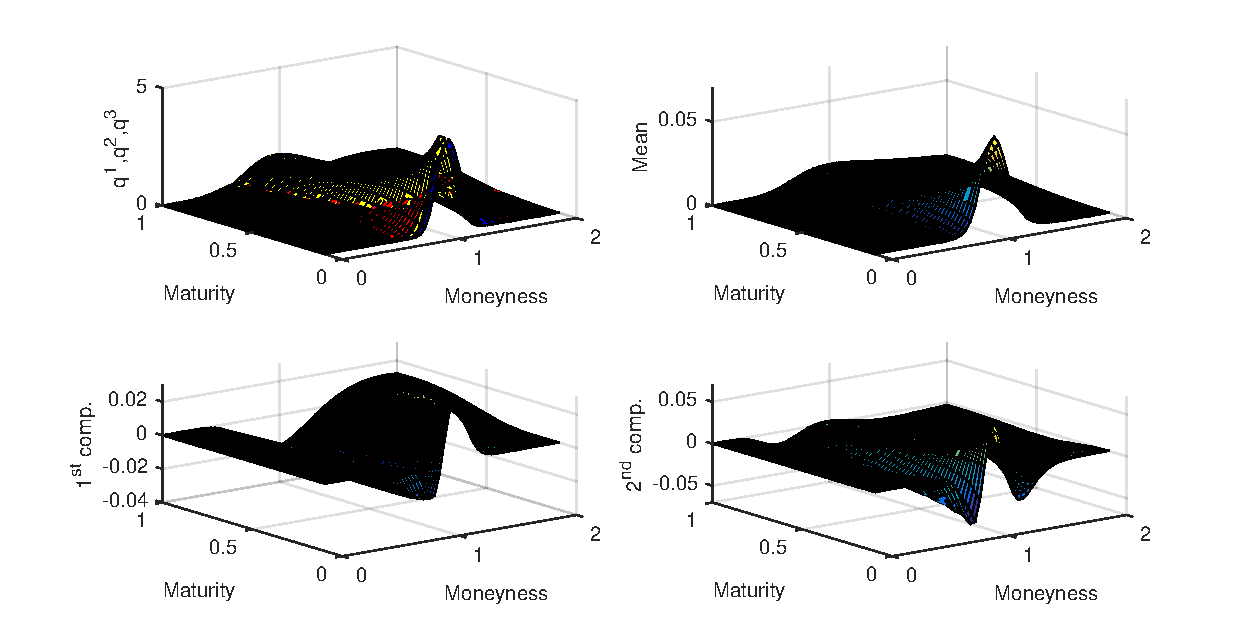
\includegraphics[width=1.00\textwidth]{Figures/Simulation2}
%\caption{\label{sim1} Simulated mixture components - log-normal densities $q^1$ - red; $q^2$ - blue; $q^3$ - yellow; Mean curve and orthonormal components}
%\end{center}
%\end{figure}


Without loss of generality, we set $r_{i\tau}=0$, for each day $i=i,\ldots,N$. %Then, in terms of the notations of section \ref{t2}, $X_i(m,\tau)=C_i(m,\tau)$ and $X_i^{(d)}(m,\tau)=q_i(m,\tau)$, for $d=(2,0)$.
%The loadings are simulated from the positive half-standard normal distribution, then standardized to sum up to one.
%Remember tat $r_{s,i}=\frac{s_i}{s_0}$. The stock price follows a geometric Brownian motion  with $\log(s_{i} / s_{i-1})\sim \mathbb{N}(0.03,0.18)$ for ordered time points $i=1,\ldots N$. The parameter choice corresponds to the empirical mean and variance of the stock index log-returns in the real data study. The starting value is $s_{0}=100$ and we fix the risk free rate to $0.02$ p.a. for all days.
We construct a random grid for each observed curve $X_i$ by simulating points $t_{ik}=(m_{ik},\tau_{ik}), \; k=1,\dots,T$ from a uniform distribution with continuous support $[0.5,1.8]\times[0.2,0.7]$. %The first dimension is moneyness and the second maturity to match the features in the real data, see next subsection.
%To get a coverage of the entire space like in the case of real data when few observations in the maturity direction are present
%We additionally require that for ordered $\tau_l$, $\EE\left[\tau_l-\tau_{l+1}\right] = \frac{1}{3}$.
Finally, we record noisy discrete observations of the call functions with additive error term i.i.d. $\varepsilon_{ik} \sim \operatorname{N}(0,0.1^2)$.%, with $\sigma_{\varepsilon}=0.02$.

%1. we know the shape of the orthogonal components
%2. identification depends on the covariance of the loadings - in our example only two are identified - it depends on the sample covariance, depending on the signal to error ratio - can be viewed as error???
%3. implied volatility variation
%By construction using a mixture of $L$ factors and $\sum_{l=1}^{L+1} w_{il}=1$ this model has $L-1$ principal components.
%The simulated components $q_l$ and their orthogonal counterparts are shown in figure \ref{?}.

%However, in our example, the third component is theoretically not identifiable. they are not always identifiable from the observations $q$ (or noisy versions of them).


%The simulated components $q$ and their orthogonal counterparts are shown in figure \ref{?}. In our example $Var(w_1)=Var(w_2)=Var(w_3)=33\%$, while the variance of the orthogonal components are $97.97\%$, $1.77\%$ and $0.26\%$ respectively.

The true SPDs given by equation (\ref{trueSPD}) are used to verify the performance of $\hat{X}^{(d)}_{i,L,\varphi}$, $\hat{X}^{(d)}_{i,L,\varphi}$ and of the individually estimated curves $\hat{X}^{(d)}_{i,LP}$ by local polynomial estimator regression. %in terms of mean integrated squared error (MSE), i.e., $T^{-1} \sum_{k=1}^T \left\{X^{(d)}(t_{ik}) - \hat{X}^{(d)}_\bullet (t_{ik})\right\}^2$, for $d=(2,0)$. For evaluation we generate a common grid of 256 points from a uniform distribution.
%the mean squared error (MSE), which averages the errors for each curve  over number of curves time observations per curve. a discrete version of N^{-1} \sum_{i=1}^N
To derive the optimal bandwidth in each case we stick to the rule-of-thumb approach presented in Section \ref{implementation}. %We adjust the rule to the given circumstance.
To illustrate the empirical performance of our estimators for the curve derivative, we compute the relative mean integrated square error

\begin{equation*}
RMISE\left(X^{(d)}_i, \hat{X}^{(d)}_{i,L,\phi}\right)=\frac{N^{-1}\sum_{i=1}^N\int_{[0,1]^g} \left\{X^{(d)}_i(t)- \hat{X}^{(d)}_{i,L,\phi}(t) \right\}^2  dt}{N^{-1}\sum_{i=1}^N\int_{[0,1]^g} \left\{X^{(d)}_i(t) \right\}^2 dt}
\end{equation*}
%\end{itemize}
Similarly, we can define $RMISE\left(X^{(d)}, \hat{X}^{(d)}_{i,L,\gamma}\right)$ and $RMISE\left(X^{(d)}, \hat{X}^{(d)}_{i,indiv.}\right)$.

The bandwidth for the individually smoothed curve $i$ is derived by replacing $\hat{p}^{(\nu)}_{ir}$ in (\ref{rulethumb}) by one and zero otherwise.
The performance is recorded for sample sizes $N$ of $10$ and $25$ with $T$ observations per day of size $50$ and $250$.  This procedure is repeated for $500$ samples to get reliable results. The mean, variance, median and the inter quartile distance based on the $RMISE $ of all samples are reported in Table \ref{fig:SimuResults}. %to show how fast the asymptotics take effect
%To show that our bandwidth criteria works, we have experimented with 100 curves. We repeated the procedure 1000 times to show how fast the asymptotics take effect.

 %In particular, for $b$ we have experimented with various bandwidths, e.g. we looked at the mean, minimum and maximum of individually optimal bandwidths. The best results are obtained for the maximum, hence, we report only these results in the following.
%Goodness of fit is measured in terms of the mean square error (MSE) per curve. We average the results for each repetition and report the sample performance using the average mean square error (AMSE).
%Their effects are evaluated in the following simulation studies.
%We considered various simulation scenarios based on the combinations of the case of errors size and number of observation points and curves.
%Tables \ref{table1} through \ref{table3} summarize the simulation results. %estimation results for curves estimated by FPCA and simple smoothing respectively. %For computing we use empirical centered true values. To guarantee a fair comparison we display AMSE for individual


%smoothed curves as well with the optimal bandwidth for individual curves and in addition for the same level of smoothing like the FPCA (marked by *). %With a single exception FPCA performs better than its benchmark model. %The distribution of AMSE is synthetized in the boxlots from figure (\ref{boxplots}).
%We need to report how the optimal constant changes with the size of the noise. If there are differences then we'll get the constant equal to the our estimated $\sigma_{\varepsilon}$ in the real data example.
%The results for the one repetition is summarized here: we find two factors because the third one is a linear function of the two. Make plot + ....
\begin{table}
\footnotesize
  \centering
  \begin{tabular}{c|c|c|c|c|c|c|c|c|c}
    \hline
    \hline
    $RMISE$&$T$&\multicolumn{4}{c|}{50}&\multicolumn{4}{c}{250}\\
    %\cline{3-6}
		\hline
    $N$&$\hat{X}^{(d)}_\bullet$&Mean&Var&Med&IQR&Mean&Var&Med&IQR\\
    \hline
    \multirow{3}{12pt}{10}	&\footnotesize $\hat{X}^{(d)}_{i,L,\varphi}$  & 0.3228 & 0.1883
 &0.1895
 &0.2333
& 0.0824
 & 0.0035
 &0.0685
&0.0536
\\
		                        &\footnotesize $\hat{X}^{(d)}_{i,L,\gamma}$& 0.2985 & 0.2233
 &0.1680
 &0.2222
& 0.0748
 & 0.0035
 &0.0580
&0.0476
\\
													  &\footnotesize $\hat{X}^{(d)}_{i,LP}$  & 0.7471& 0.7545
 &0.4959
 &0.6329
& 0.1447
 & 0.0106

 &0.1150
&0.1035
\\
								\hline
    \multirow{3}{12pt}{25}  &\footnotesize $\hat{X}^{(d)}_{i,L,\varphi}$& 0.1735  & 0.0389
 &0.1218
&0.1148
& 0.0610
&0.0008
 & 0.0528
 &0.0419
\\
		                        &\footnotesize $\hat{X}^{(d)}_{i,L,\gamma}$& 0.1532  & 0.0363
 &0.1012
&0.0978
& 0.0467
&0.0014
 & 0.0405
 &0.0266
\\
											 	  	&\footnotesize $\hat{X}^{(d)}_{i,LP}$ & 0.8083  & 0.8215
 &0.5418
&0.6778
& 0.1457
&0.0105
 & 0.1177
&0.1039
\\
    \hline  \hline
  \end{tabular}
  \caption{Simulation results for $g=2$. Based on the mean and the median of $RMISE$, $\hat{X}^{(d)}_{i,L,\varphi}$ and $\hat{X}^{(d)}_{i,L,\gamma}$ yield superior results compared to $\hat{X}^{(d)}_{i,h}$ and $\hat{X}^{(d)}_{i,L,\gamma}$ outperforms $\hat{X}^{(d)}_{i,L,\varphi}$ in all cases. Results for $\hat{X}^{(d)}_{i,L,\varphi}$ and $\hat{X}^{(d)}_{i,L,\gamma}$ improve with raising $N$ and $T$. These results support our asymptotic results given by Proposition \ref{Mbias} and \ref{curvebias}. }
  \label{fig:SimuResults}
  \href{https://github.com/QuantLet/FPCA/tree/master/FPCAsimulation}{\color{black} \quantnet FPCAsimulation}
\end{table}


%
%\begin{center}
%\textbf{[Insert Table~\ref{table1} approximately here.]}
%\end{center}
%\begin{center}
%\textbf{[Insert Table~\ref{table2} approximately here.]}
%\end{center}
%\begin{center}
%\textbf{[Insert Table~\ref{table3} approximately here.]}
%\end{center}

Both FPCA based approaches give better estimates for the derivative of the call functions than an individually applied local polynomial estimator of the individual curves. Both the mean and the median of the $RMISE $ are smaller which is a result of the additional average over $N$ for the basis functions as given by Proposition \ref{curvebias}. However, the $\hat{X}^{(d)}_{L,i,\gamma}$ performs decisively better for small $T$ than the other two both in terms of mean and standard deviation of the mean squared error.
In addition $\hat{X}^{(d)}_{L,i,\gamma}$ benefits more from increasing $N$ than $\hat{X}^{(d)}_{L,i,\varphi}$. With small $T$ for $\hat{X}^{(d)}_{L,i,\varphi}$ and individual smoothing the variability of $RMISE$ is much bigger than for $\hat{X}^{(d)}_{L,i,\gamma}$ while the median of $RMISE$ for $\hat{X}^{(d)}_{L,i,\gamma}$ and $\hat{X}^{(d)}_{L,i,\varphi}$ are comparable. This means individual local polynomial smoothers and $\hat{X}^{(d)}_{L,i,\varphi}$ must behave much worse than $\hat{X}^{(d)}_{L,i,\gamma}$ in some instances while $\gamma^{(d)}_r$-based expansion was able to stabilize the estimates. To get the same effect using $\hat{X}^{(d)}_{L,i,\varphi}$ a much bigger $T$ is needed. A possible explanation for this behavior is given by Proposition \ref{Mbias}. The rates of convergence for the estimators of the dual matrix entries rely on $T$. Thus in finite sample, when $T$ is small, the estimated loadings might be biased. %The rates of convergence for the estimators of the dual matrix entries rely on $T$, thus when facing small $T$ some of the estimated loadings might be inaccurate.
%For all estimation procedures the interquartile range (IQR) together with the standard deviation suggests that the distribution of MSE has fatter tails than normal and the comparison of mean and median also suggests a non normal distribution. %, in particular for the direct method.

%Its performance depends on the sample characteristics and using it in applications has an associated higher risk.
%In addition, the slow improvement in the direct method confirm that the order of convergence is dominated by the fixed number of observations per curve $T$. %the sample size of curves shall be very large to give comparable convergence with the indirect method. \color{red}Also possible that it never does, we need to increase the observation points. (Unless we increase the observation points ... it will never be asymptotically equivalent???) \color{black}


%Contrasting the interquartile range (IQR) with the standard deviation suggests that the distribution of MSE has fatter tails than normal, in particular for the direct method.

%In particular, the direct method has many Looking at the IQR suggests that the large variance is due to the very bad performance of FPCA_2 in some of the cases (not necessarily outliers). The standard deviation stabilizes when we increase the number of curves (or not?). the small improvement in the fpca2 suggests that the number of curves shall be much higher.


We provided empirical performance results for $\hat{\gamma}^{(d)}_{r,T}$ and $\hat{\varphi}^{(d)}_{r,T}$ based on the relative integrated square error

%\begin{equation*}
%RISE\left(\varphi^{(d)}_r, \hat{\varphi}^{(d)}_{r,T}\right)=\frac{\int_{[0,1]^g} \left\{\varphi^{(d)}_{r}(t)- \hat{\varphi}^{(d)}_{r,T}(t) \right\}^2  dt}{\int_{[0,1]^g} \left\{\varphi^{(d)}_{r,T}(t) \right\}^2 dt}
%\end{equation*}

\begin{equation*}
RISE\left(\gamma^{(d)}_r, \hat{\gamma}^{(d)}_{r,T}\right)=\frac{\int_{[0,1]^g} \left\{\gamma^{(d)}_{r}(t)- \hat{\gamma}^{(d)}_{r,T}(t) \right\}^2  dt}{\int_{[0,1]^g} \left\{\gamma^{(d)}_{r,T}(t) \right\}^2 dt}.
\end{equation*}
By definition, the denominator of $RISE\left(\varphi^{(d)}_r, \hat{\varphi}^{(d)}_{r,T}\right)$ is zero.



\begin{table}
\footnotesize
  \centering
  \begin{tabular}{c|c|c|c|c|c|c|c|c|c}
    \hline
    \hline
    \multicolumn{2}{c|}{$RISE}$&\multicolumn{4}{c|}{Mean}&\multicolumn{4}{c}{Median}\\
    %\cline{3-6}
		\hline
    $N$&$T$&$\hat{\gamma}^{(d)}_{1,T}$&$\hat{\gamma}^{(d)}_{2,T}$&$\hat{\varphi}^{(d)}_{1,T}$&$\hat{\varphi}^{(d)}_{1,T}$&$\hat{\gamma}^{(d)}_{1,T}$&$\hat{\gamma}^{(d)}_{2,T}$&$\hat{\gamma}^{(d)}_{1,T}$&$\hat{\varphi}^{(d)}_{2,T}$\\
    \hline
    50 & 10	&19.97	&	6.99	&	0.91	&	1.02	&	2.69	&	0.05	&	0.96	&	1.02
\\
		  250 & 10  &51.7	&	1.35	&	0.64	&	1.03	&	2.54	&	0.19	&	0.6	&	1.06
\\

								\hline
    50 & 25  & 9.02	&	0.24	&	0.84	&	1.01	&	0.96	&	0.05	&	0.87	&	1.03
\\
	250 & 25	                      & 3.22	&	1.54	&	0.54	&	1.06	&	0.49	&	0.19	&	0.45	&	1.09
\\
    \hline  \hline
  \end{tabular}
  \caption{Simulation results for $g=2$.
	Based on the mean and the median of $RISE$, $\hat{\gamma}^{(d)}_{r,T}$ and $\hat{\varphi}^{(d)}_{r,T}$ improve with raising $N$ and $T$. %These results support our asymptotic results given by Proposition \ref{Mbias} and \ref{curvebias}.
	}
  \label{tab:plmbais}
  %\href{https://github.com/QuantLet/FPCA/tree/master/FPCAsimulation}{\color{black} \quantnet FPCAsimulation}
\end{table}



The results are summarized in Table \ref{tab:plmbais}. The mean and median of $RISE$ do not have the same order of magnitude and the the results for the corresponding $r$ are not comparable because they refer to different functions $\hat{\varphi}^{(d)}_{r,T}$ and $\hat{\gamma}^{(d)}_{r,T}$. %two different quantities. \textit{since the two quantities are of a different order of magnitude (btw. a possible way out is to normalize $\phi$ - I think the convexity of the function might matter as well, not sure).}
%Instead
To compare our method with existing benchmark, we included a simulation study for the unidimensional case, in which we report the results obtained with our second method presented in equations \eqref{der2} and \eqref{pder2} and the results of \cite{Mueller:2009}, since both these two approaches aim to estimate $\gamma^{(d)}_{r}$.  % estimated functions are included in Section \ref{simstudy} and explained below.


%\bigskip

%To evaluate the finite sample performance of (both) our methods with the method proposed by \cite{Mueller:2009}, we investigate the case $g=1$, which has been described in their paper.
Implementing the method of \cite{Mueller:2009} is very slow because the double sum in their equation (7). Therefore, we use their Matlab code available on one of the author's personal website, based on binning. We experimented with different binning points and chose to report the best performance results obtained with 15 points. We use an Epanechnikov kernel, the true number of componentswe keep the default values in the code. We simulate call prices for the fixed time to maturity $\tau=0.5$ years, for different $N$ and $T$, perform 500 replications and report the mean and median of the relative mean integrated square errors, and of the absolute error respectively. The error standard error is $\sigma_{\varepsilon}=0.005$. The relative performance criteria of the two methods is showed in Table \ref{taplcurves} and Table \ref{taplcurves2}.

%Results show

\begin{table}
\footnotesize
  \centering
  \begin{tabular}{c|c|c|c|c|c|c|c|c|c}
    \hline
    \hline
    \multicolumn{2}{c|}{}&\multicolumn{4}{c|}{$RMISE\left(X^{(d)}, \hat{X}^{(d)}_{i,L,\gamma}\right)$}&\multicolumn{4}{c}{$RMISE\left(X^{(d)}, \hat{X}^{(d)}_{i,LM}\right)$}\\
    %\cline{3-6}
		\hline
    $N$&$T$&Mean&Var&Med&IQR&Mean&Var&Med&IQR\\
    \hline
    25 & 25	&2.74	&	26.3	&	0.84	&	1.36	&	2.77	&	26.83	&	1.74	&	2.42	\\
		  50 & 25                   & 0.55	&	8.67	&	0.4	&	0.39	&	2.58	&	10.88	&	1.16	&	2.4	\\
		  200 &25                   & 0.21	&	0.25	&	0.16	&	0.15	&	0.84	&	9.49	&	0.59	&	0.54	\\
								\hline
    25 & 50  &13.98	&	18.48	&	0.74	&	1.15	&	2.03	&	12.4	&	1.19	&	1.8	\\
	50 & 50	                      & 0.44	&	19.92	&	0.3	&	0.3	&	1.88	&	6.07	&	0.89	&	1.75	\\
		  200 &50                 & 0.14	&	0.12	&	0.11	&	0.1	&	0.64	&	5.37	&	0.47	&	0.42	\\
								\hline
    25 & 200   & 0.59	&	0.99	&	0.7	&	1.31	&	1.38	&	3.92	&	0.66	&	1.24	\\
	50 & 200	                      & 0.24	&	0.67	&	0.18	&	0.17	&	1.41	&	3.37	&	0.64	&	1.29	\\
		  200 &200                 & 0.07	&	0.03	&	0.06	&	0.06	&	0.33	&	0.96	&	0.26	&	0.24	\\
    \hline  \hline
  \end{tabular}
  \caption{Simulation results for $g=1$.
	Based on the mean and the median of $RMISE$, $\hat{X}^{(d)}_{i,L,\gamma}$ performs better than $\hat{X}^{(d)}_{i,LM}$ in all cases. Results for $\hat{X}^{(d)}_{i,L,\gamma}$ and $\hat{X}^{(d)}_{i,LM}$ improve with raising $N$ and $T$. %These results support our asymptotic results given by Proposition \ref{Mbias} and \ref{curvebias}.
	}
  \label{taplcurves}
  %\href{https://github.com/QuantLet/FPCA/tree/master/FPCAsimulation}{\color{black} \quantnet FPCAsimulation}
\end{table}



\begin{table}
\footnotesize
  \centering
  \begin{tabular}{c|c|c|c|c|c|c|c|c|c}
    \hline
    \hline
    \multicolumn{2}{c|}{$RISE$}&\multicolumn{4}{c|}{Mean}&\multicolumn{4}{c}{Median}\\
    %\cline{3-6}
		\hline
    $N$&$T$&$\hat{\gamma}^{(d)}_{1,T}$&$\hat{\gamma}^{(d)}_{2,T}$&$\hat{\gamma}^{(d)}_{1,LM}$&$\hat{\gamma}^{(d)}_{2,LM}$&$\hat{\gamma}^{(d)}_{1,T}$&$\hat{\gamma}^{(d)}_{2,T}$&$\hat{\gamma}^{(d)}_{1,LM}$&$\hat{\gamma}^{(d)}_{2,LM}$\\
    \hline
    25 & 25	&15.07	&	58.94	&	10.78	&	8.54	&	5.5	&	18.62	&	8.61	&	7.73
\\
		  50 & 25                   & 3.71	&	18.83	&	7.42	&	7.39	&	2.57	&	11.3	&	6.85	&	7.16
\\
		  200 &25                   & 1.48	&	11.68	&	11.3	&	56.82	&	1.27	&	7.59	&	6.05	&	32.9
\\
								\hline
    25 & 50   & 16.78	&	25.46	&	8.19	&	7.39	&	5.46	&	17.74	&	7.33	&	7.13
\\
	50 & 50	                      & 2.54	&	17.33	&	6.67	&	7.03	&	1.98	&	9.73	&	6.35	&	6.94
\\
		  200 &50                 & 1.00	&	7.19	&	6.33	&	33.56	&	0.83	&	4.95	&	3.47	&	17.26
\\
								\hline
    25 & 200  & 11.96	&	18.93	&	6.64	&	6.56	&	4.61	&	20.97	&	6.39	&	6.48
\\
	50 & 200	                      & 1.43	&	10.02	&	6.31	&	6.84	&	1.15	&	7.59	&	6.23	&	6.82
\\
		  200 &200                 & 0.47	&	3.78	&	2.44	&	12.97	&	0.42	&	2.78	&	1.71	&	9.03
\\
    \hline  \hline
  \end{tabular}
  \caption{Simulation results for $g=1$. Based on the median of $RMSE$, $\hat{\gamma}^{(d)}_{1,T}$ performs better than $\hat{\gamma}^{(d)}_{1,LM}$. In general, results for both $\hat{\gamma}^{(d)}_{1,T}$ and $\hat{\gamma}^{(d)}_{1,LM}$  improve with raising $N$ and $T$.  %yield superior results compared to $\hat{X}^{(d)}_{i,h}$ and $\hat{X}^{(d)}_{i,L,\gamma}$ outperforms $\hat{X}^{(d)}_{i,L,\varphi}$ in all cases. Results for $\hat{X}^{(d)}_{i,L,\varphi}$ and $\hat{X}^{(d)}_{i,L,\varphi}$ improve with raising $N$ and $T$. These results support our asymptotic results given by Proposition \ref{Mbias} and \ref{curvebias}.
	}
  \label{taplcurves2}
  %\href{https://github.com/QuantLet/FPCA/tree/master/FPCAsimulation}{\color{black} \quantnet FPCAsimulation}
\end{table}




\subsection{Real Data Example }%\color{red}we only report results by our method\color{black}
\label{realData}
\subsubsection{Data description }We use settlement European call option prices written on the underlying DAX 30 stock index. These prices are computed by EUREX at the close of each trading day as an average of the intraday transaction prices. The data range is ten years, between January 2, 2002 and December 3, 2011, and includes 2557 days. %The data set was accessed through the Research Data Center (RDC) at the CRC 649.
The expiration dates of the options are set on the third Friday of the month. Therefore, on a particular day, option prices with only a few maturities are available, see Figure~\ref{exp}. The distance between two consecutive observed maturities is higher for more distant expiration dates, while the distance between two consecutive strike prices is relatively constant. Methods that analyze curves jointly are generally better tailored to this type of data, because they provide better estimates at grid points with only a few observations available of the individual curves. % with only a few maturities available every day
% Often in practice, the call and SPD surfaces are obtained by interpolating two one-dimensional smooth curves, with closest maturities. In our application, the partial derivative in the moneyness direction is zero and using local polynomial method produces smooth estimates and interpolates in one step. This data structure is better tailored to by analyzed  the curves together than individually. This data structure, with only a few available maturities daily, still allow the use of local polynomial method for smoothing in our application because the estimates in the maturity direction can be interpreted as weighted averages of the neighboring estimates for fixed observed maturities. %This is similar to interpolation that is often used in practice for option prices. %For this data structure containing sparse areas for high maturities, the nearest-neighbor interpolation method introduces potentially high bias since the call options are known to vary monotonically with the strike and the expiration date. Therefore, we choose instead the linear interpolation to get the curves on the common grid. In this setup, this gives better results in finite sample than the nearest neighborhood method.
We include call options with maturity between one day and one year. The sample contains prices of options with an average of six maturities and sixty-five strikes per day. % From these data we We don't use all these data because of truncations requited by finding the maximum overlapping domain over all curves.

By assuming 'sticky' coordinates for the daily observations, in accordance with equation \eqref{q10}, we divide the strike and the call prices within one day by the stock index forward price to ensure that the observation points are in the same range. %the observed options occur on the same range of relative strikes, that is our moneyness metrics $m$. %\color{red}Observations of each curve $C_i$ no longer occur at the same grid points. We use nearest neighborhood (in moneyness direction) and linear (in maturity direction) interpolation to compute the values of the call prices on an equidistant grid defined as the maximum common domain of observations in both dimensions. Our choice for the interpolation points is: thirty-one distinct grid points for the moneyness and twenty for the maturity. For simplicity, we treat them as direct observations further on. Consequently, we apply the FPCA to noisy standardized call prices and estimate their second derivative with respect to $m$ in a fixed design setup.\color{black}
%(The treatment of random design was already discussed in section.)%$T=[  \underset{t}{\left\{ \operatorname{max}} \left(\underset{j}{\operatorname{min}} R_{t,j}\right) \right\} ]x[]$.
%In order to retrieve the estimated SPDs we also need risk free interest rate daily data for various maturities, see equation \eqref{q09}. We derive a proxy for these based on the term structure of the LIBOR rate. We compute the corresponding annual interest rate by linearly interpolating the available LIBOR rates on a daily base.
%In the real data application we do not pre-multiply the daily observations with the corresponding $\exp{(r_{i,\tau},\tau)}$  in equation (\ref{q09}) and report the results of the FPCA decomposition in terms of equation (\ref{q}). %The implicit assumption is that for the considered time frame the risk free interest rate is constant.
%Following the methodological framework,
Afterwards, we apply the estimation methodology described in Section \ref{t2} to the rescaled call prices as a function of moneyness and maturity. % points and report the decomposition results for their second derivative with respect to moneyness. %As a consequence, the estimated components have not been adjusted to account for the interest rate term structure in the maturity direction and its daily variability is incorporated in the loadings. To obtain the SPD on a particular day $i$ we need to multiply the second derivative of the call prices obtained from a reduced form model by $\exp{(r_{i,\tau}\tau)}$ for each maturity $\tau$, see equation (\ref{q09}). If one is interested in the SPD dynamics rather than in the call derivative, an alternative to this procedure is to pre-multiply the daily call observations by the corresponding discount factors
%$\exp{(r_{i,\tau},\tau)}$
%and afterwards apply FPCA to the adjusted prices. Each choice is best fitted to a particular research goal.
%For illustrating our framework and for the purpose of comparing our results with the empirical literature on the implied volatility surfaces we considered the first approach better suited.
Our proxy for the risk-free
interest rates are the EURIBOR rates, which are listed daily for several maturities. We apply a linear interpolation to calculate the rate values for desired maturities.% variation of the interest rate can be corrected for subsequently, if one is interested in the shape of the SPD on a particular.
%This is achieved by considering daily yield term for discounting in the moneyness direction.

%We do not pre-multiply the daily observations with the corresponding $\exp{(r_{i,\tau},\tau)}$  in equation (\ref{q09})

%In our subsequent analysis, we use the VDAX index computed by Deutsche B{\"o}rse AG from the prices of call and put options. This index reflects the market expectation under the risk neutral measure of the 30 day ahead square root implied variance for the DAX 30 log-returns, which is then annualized.


\subsubsection{Estimation results } We report the results for the loadings estimated by spectral decomposition of dual covariance matrix for option price functions, and the estimates of the second partial derivative of the functional principal components.  %The implementation of criteria (\ref{optk}) for the choice of $L$ and $L_d$ suggests a three factors for the call option surfaces dynamics, and two-factors for the dynamics of state price density surfaces, see also figure \ref{basis}. The first three and two respectively largest eigenvalues explain a disproportionate amount of variance compared to the subsequent ones, which are all close to zero. %, depending on the choice of $K_{\max}$.
%The implementation of criteria (\ref{optk}) for the choice of $L$ suggests at least three and for $L_d$ two components. The corresponding largest eigenvalues of the covariance operators for the call option and state price density surfaces are much larger then the subsequent ones, which are either close to zero or approach zero after a few other components (figure \ref{?}). This implies that we can use a factor model as in (\ref{approx11}) to represent the dynamics of state price density surfaces. Since the theoretical and simulation results recommend using the decomposition (\ref{der2}) over (\ref{pder2}) for estimating derivatives, we report the results obtained by the estimation and eigendecomposition of $M^{(0)}$. The error surface ....
The first eigenvalue of the dual covariance matrix $\hat{M}^{(0)}$ for the call option surfaces has a dominant explanatory power. The order of magnitude of the following eigenvalues decreases by a factor of ten for every few additional components.
%starting with the third component the eigenvalues have the same order of magnitude. %the following components decay fast.
%, see Table \ref{baing}. % and approach zero after a few other components \color{red}(test for lambda=0)\color{black}.
To detect the relative contribution of consecutive components, we construct the ratio of two adjacent estimated eigenvalues in descending order, see \cite{Ahn2013}. The first two terms are dominating the sequence and there are spikes at the fourth and seventh component ratio. %, before the sequence decreases towards one. %approaches one from above. %stabilizes close to one. %The largest value of this ratio - if we ignore the first component - gives three components, and the ratio stabilizes around one only after the ninth component.
%The evaluation of the information criterion of \cite{Bai2002}, see equation (\ref{optk}) for the choice of $L$, has a minimum at $k=3$ for $L_{max}=2$. Further evaluations of the criterion suggest up to eleven components.  We report the case $L=3$, which is an upper bound for $L_d$. We also discuss subsequently the effect of including additional factors on the stability of results.
%The choice of the maximum number of factors by the
$PC^{(0)}$ criterion suggests at least seven components, see values of $k^*$ for $L_{max}\geq 7$ in Table \ref{baing}. %, which are independent of the constrain $k\leq L_{max}$ in the objective function (\ref{optk}). %and its unconstrained equivalent ($k \in \mathbb{N}$) are identical for $L_{max}\geq 7$, marked bold in Table \ref{baing}. %, (it is minimized at $L_{\max}$ for $L_{\max} \leq 6$).
$IC^{(0)}$ criterion, which does not depend on the truncation parameter $L_{max}$, suggests seven components. %We refer below to the first eight estimated components. %We report below the upper bound case $L_d\leq 8$.
%case $L=7$, which is an upper bound for $L_d$.% We also discuss subsequently the effect of including additional factors on the stability of results. % hereafter a parsimonious factor model with
%This implies an upper bound on $L_d$ of maximum three components.
\begin{table}[ht]
\begin{center}
\begin{tabular}{c|r@{.}l  r@{.}l  r@{.}l  r@{.}l  r@{.}l  r@{.}l  r@{.}l  r@{.}l  r@{.}l  r@{.}l}\hline\hline      $r$,     $L_{\max}$ &\multicolumn{2}{c}{1}&\multicolumn{2}{c}{2}&\multicolumn{2}{c}{3}&\multicolumn{2}{c}{4}&\multicolumn{2}{c}{5}&\multicolumn{2}{c}{6}&\multicolumn{2}{c}{7}&\multicolumn{2}{c}{8}&\multicolumn{2}{c}{9}&\multicolumn{2}{c}{10}\\ \hline
  %\multicolumn{2}{c}{r=1}&\multicolumn{2}{c}{r=2}&\multicolumn{2}{c}{r=3}&\multicolumn{2}{c}{r=4}&\multicolumn{2}{c}{r=5}&\multicolumn{2}{c}{r=6}&\multicolumn{2}{c}{r=7}&\multicolumn{2}{c}{t=8}&\multicolumn{2}{c}{r=9}&\multicolumn{2}{c}{r10}\\ \hline
 $\hat{\lambda}_{r,T}\times 10^{6}$&  133&29 & 18&90 &  2&69&  1&62 &  0&49 &  0&34 &  0&26  & 0&09 &  0&08  & 0&05\\
  % $\lambda_r\times 10^{6}$&  144&49 & 12&00 &  4&36 &  1&08  &  0&87 &  0&37 &  0&17  & 0&14 &  0&08  & 0&03\\
 % $\lambda_r^{(d)}\times 10^{6}$&   63&66 & 23&86 &  6&77 & 4&81 &  2&47 &   1&03  &  0&78  &  0&57  &  0&54  & 0&41\\  \hline
%  $\hat{\lambda}_{r,T}^{(d)}\times 10^{2}$&   14&74 & 3&76 &  2&83 & 2&14 &  1&12 &   0&80  &  0&20  &  0&19  &  0&515  & 0&12\\  \hline
 % $\lambda_r /  \lambda_{r+1}$&   12&04  &  2&76  &  4&02  &  1&25 &  2&37 &  2&15 & 1&20  & 1&81  &  2&47 &  1&26\\
   $\hat{\lambda}_{r,T} /  \hat{\lambda}_{r+1,T}$&   7&05  &  7&01  &  1&66  &  3&28 &  1&44 &  1&31 & 2&83  & 1&18  &  1&70 &  1&35\\
 %$\lambda_r^{(d)} / \lambda_{r+1}^{(d)}$&  2&67  &  3&52 &  1&41 &  1&95  &  2&39  &  1&32  &  1&36  &  1&06 &  1&30  &  1&55\\    \hline
% $\hat{\lambda}_{r,T}^{(d)} / \hat{\lambda}_{r+1,T}^{(d)}$&  3&92  &  1&33&  1&32 &  1&92  &  1&40  &  4&01  &  1&04 &  1&23 &  1&27  &  1&37\\    \hline %$L$&\multicolumn{2}{c}{N/A}&\multicolumn{2}{c}{3}&\multicolumn{2}{c}{4}&\multicolumn{2}{c}{5}&\multicolumn{2}{c}{6}&\multicolumn{2}{c}{6}&\multicolumn{2}{c}{8}&\multicolumn{2}{c}{9}&\multicolumn{2}{c}{9}&\multicolumn{2}{c}{9}\\

%$k^*(PC^{(0)})$&\multicolumn{2}{c}{1}&\multicolumn{2}{c}{2}&\multicolumn{2}{c}{3}&\multicolumn{2}{c}{4}&\multicolumn{2}{c}{5}&\multicolumn{2}{c}{6}&\multicolumn{2}{c}{\textbf{7}}&\multicolumn{2}{c}{\textbf{8}}&\multicolumn{2}{c}{\textbf{9}}&\multicolumn{2}{c}{9}\\
$k^*(PC^{(0)})$&\multicolumn{2}{c}{-}&\multicolumn{2}{c}{-}&\multicolumn{2}{c}{-}&\multicolumn{2}{c}{-}&\multicolumn{2}{c}{-}&\multicolumn{2}{c}{-}&\multicolumn{2}{c}{7}&\multicolumn{2}{c}{8}&\multicolumn{2}{c}{9}&\multicolumn{2}{c}{9}\\

$k^*(IC^{(0)})$&\multicolumn{2}{c}{-}&\multicolumn{2}{c}{-}&\multicolumn{2}{c}{-}&\multicolumn{2}{c}{-}&\multicolumn{2}{c}{-}&\multicolumn{2}{c}{-}&\multicolumn{2}{c}{7}&\multicolumn{2}{c}{-}&\multicolumn{2}{c}{-}&\multicolumn{2}{c}{-}\\
%$L_d$&\multicolumn{2}{c}{N/A}&\multicolumn{2}{c}{3}&\multicolumn{2}{c}{4}&\multicolumn{2}{c}{5}&\multicolumn{2}{c}{5}&\multicolumn{2}{c}{5}&\multicolumn{2}{c}{6}&\multicolumn{2}{c}{7}&\multicolumn{2}{c}{9}&\multicolumn{2}{c}{10}\\

%$k^*(PC^{(d)})$&\multicolumn{2}{c}{-}&\multicolumn{2}{c}{-}&\multicolumn{2}{c}{-}&\multicolumn{2}{c}{-}&\multicolumn{2}{c}{-}&\multicolumn{2}{c}{-}&\multicolumn{2}{c}{6}&\multicolumn{2}{c}{8}&\multicolumn{2}{c}{9}&\multicolumn{2}{c}{10}\\
%$k^*(PC^{(d)})$&\multicolumn{2}{c}{1}&\multicolumn{2}{c}{2}&\multicolumn{2}{c}{3}&\multicolumn{2}{c}{4}&\multicolumn{2}{c}{5}&\multicolumn{2}{c}{\textbf{6}}&\multicolumn{2}{c}{6}&\multicolumn{2}{c}{\textbf{8}}&\multicolumn{2}{c}{\textbf{9}}&\multicolumn{2}{c}{\textbf{10}}\\
% $k^*(PC^{(d)})$&\multicolumn{2}{c}{1}&\multicolumn{2}{c}{2}&\multicolumn{2}{c}{3}&\multicolumn{2}{c}{4}&\multicolumn{2}{c}{5}&\multicolumn{2}{c}{5}&\multicolumn{2}{c}{6}&\multicolumn{2}{c}{7}&\multicolumn{2}{c}{9}&\multicolumn{2}{c}{10}\\
%\hline
%$r'$&\multicolumn{2}{c}{1}&\multicolumn{2}{c}{2}&\multicolumn{2}{c}{7}&\multicolumn{2}{c}{6}&\multicolumn{2}{c}{8}&\multicolumn{2}{c}{3}&\multicolumn{2}{c}{9}&\multicolumn{2}{c}{5}&\multicolumn{2}{c}{4}&\multicolumn{2}{c}{15}\\
\hline\hline
    \end{tabular}
\caption{\label{baing} Estimated eigenvalues and eigenvalue ratios. Number of factors by $PC^{(0)}$ criterion} %Index of sorted component $\hat{\gamma}_{r,T}$ in decreasing order for explained variance}
\footnotesize  \href{https://github.com/QuantLet/FPCA/tree/master/FPCAreal_data}{\color{black} \quantnet FPCArealdata}
\end{center}
\end{table}

\begin{figure}[ht]
\begin{center}
%\includegraphics[width=1.00\textwidth]{figures/Callssecondloadings75} \\
%\includegraphics[width=1.00\textwidth]{figures/Callssecondloadings76}
\includegraphics[width=1.00\textwidth]{Figures/CallsloadingsNEWforward1392}
%\caption{\label{second_comp} Left: Call options on the expiration day. Right: Second non-orthogonal component $\hat{\gamma}_{2,T}$}
\caption{\label{exp} The effect of expiration date on the level of estimated loadings $\hat{\delta}_{2,T}$ }
\footnotesize \href{https://github.com/QuantLet/FPCA/tree/master/FPCAexpiration}{\color{black}\quantnet FPCAexpiration}
\end{center}
\end{figure}


%A closer look at the dynamics of the loadings, shows an unusual behavior of some of them - $\hat{\delta}_{2,T}$, $\hat{\delta}_{4,T}$, $\hat{\delta}_{5,T}$ and $\hat{\delta}_{6,T}$ - between mid-February 2007 through mid-June 2008.
A closer look at the dynamics of the loadings $\hat{\delta}_{2,T}$ shows an unusual behavior between mid-February 2007 through mid-June 2008.
This interval spans the financial crisis and extends until the end of the recession in the Euro Area, according to the Center for Economic and Policy Research (CEPR) recession indicator. %It shows a recession from the period following the peak through the trough -
The loadings are extremely volatile and display a particular time regularity of jumps. We identify these jumps with the Mondays following an expiration date (options expire at a monthly frequency, always on a Friday). Figure \ref{exp} highlights the dynamics of $\hat{\delta}_{2,T}$ on and following an expiration day. After roughly two weeks, the loadings revert to a 'normal' level. %After the sudden decrease, the loadings increase day-by day and approach a 'normal' level after about two weeks. %, as the string of options with the smallest available maturity approaches expiration.
%During this period, the call prices for small maturities are extremely convex at-the-money and the absence of a call string with close enough small maturity on the following trading Monday leads to severe bias in the values of $\hat{C}^{(\nu)}_{i,b}(m,\tau)$, estimated through equation (\ref{polyeqkern}), for $\tau<\min(\tau_i)$.
During this period, for small maturities, there are only few observations available for call prices with strikes larger than the current stock index. In addition, the absence of a call string with close enough time to maturity on the following trading Monday, introduces bias in the estimated smooth call surface for grid values outside the observation points range. %, stemming from the extrapolation problem for the local kernel regressions.
 %is not due to an error in pre-smoothing of the call options used for the estimation of $M^{(0)}$ because even if we recalculate the explained variance for all the components after excluding the estimated loadings from this time interval, this factor still remains the second most important.
%We cannot, however, downplay the importance of this component because it remains the second most important in terms of variance explained if we remove this time interval from the sample.
The shape of the second estimated component $\hat{\gamma}^{(d)}_{2,T}$, displayed in Figure \ref{exp}, suggests that it is related to variations of the short end of the SPD term structure. %The other components $\hat{\gamma}_{4,T}$, $\hat{\gamma}_{5,T}$, $\hat{\gamma}_{6,T}$ and $\hat{\gamma}_{8,T}$, whose loadings have similar jump-behavior, are similar in shape to the four components we have discussed so far, i.e., $\hat{\gamma}_{1,T}$, $\hat{\gamma}_{2,T}$, $\hat{\gamma}_{3,T}$ and $\hat{\gamma}_{7,T}$. We contend that they are related to the asymmetric behavior of the option prices along the maturity direction, i.e., the term structure effect of the SPDs. %- more than one factor is necessary to explain the variation in the time to maturity direction. %We therefore focus on the remaining three components. %The evidence indicate is an indicative that the importance of the second component is due to an error in pre-smoothing of the call options used for the estimation of $M^{(0)}$, and we exclude it from our further analysis. Note that even if we recalculate the explained variances for all the components after removing the loadings from this time interval, this factor still remains important, \color{red}which may imply that the smoothing error affects the results for our entire sample \color{black}. Further, we look at the shape of the other components and the dynamics of their corresponding loadings. The loadings of components $\hat{\gamma}_{4,T}$, $\hat{\gamma}_{5,T}$ and $\hat{\gamma}_{6,T}$ suffer from the same problem as $\hat{\delta}_{2,T}$. We therefore remove them from the candidate factors. \color{red} ???? they are related to short term effects. \color{black}
A similar behavior of the loadings are observed for a few other components we investigated: $\hat{\delta}_{4,T}$, $\hat{\delta}_{5,T}$ and $\hat{\delta}_{6,T}$. Their variances remain important even if we exclude the interval with large jumps from the sample. The corresponding components have similar shape features to the three components we discuss below. We argue that they impact the option prices and SPDs when jumps in the underlying occur, and that they related to the asymmetric behavior of the option prices along the maturity direction. %, the term structure effect of the SPDs.  . %and impact the options with different maturities differently.



%these components have a significant impact on option re- turns even in the presence of stock market and volatility jumps

%Further $\hat{\gamma}^{(d)}_{4,T}$, $\hat{\gamma}^{(d)}_{4,T}$, $\hat{\gamma}^{(d)}_{7,T}$ and $\hat{\gamma}^{(d)}_{8,T}$ are similar in shape to $\hat{\gamma}_{2,T}$ and


%We further report on the other the case $L=3$, which is an upper bound for $L_d$. We also discuss subsequently the effect of including additional factors on the stability of results. For visualization, we multiply the estimated components by the standard deviation of the corresponding loadings.
%\begin{figure}[ht]
%\begin{center}
%\includegraphics[width=1.00\textwidth]{figures/phi6}
%\caption{\label{ort} First six orthogonal components obtained by the decomposition of $\hat{M}^{(0)}$}
%\includegraphics[width=1.00\textwidth]{figures/phi}
%\caption{\label{ort} First eight orthogonal components obtained by the decomposition of $\hat{M}^{(0)}$}
%\end{center}
%\end{figure}

\begin{figure}[ht]
\begin{center}
%\includegraphics[width=1.0\textwidth]{figures/Nonorthogonalbasis20160502}
\includegraphics[width=1.0\textwidth]{figures/Nonorthogonalbasis20160605}
%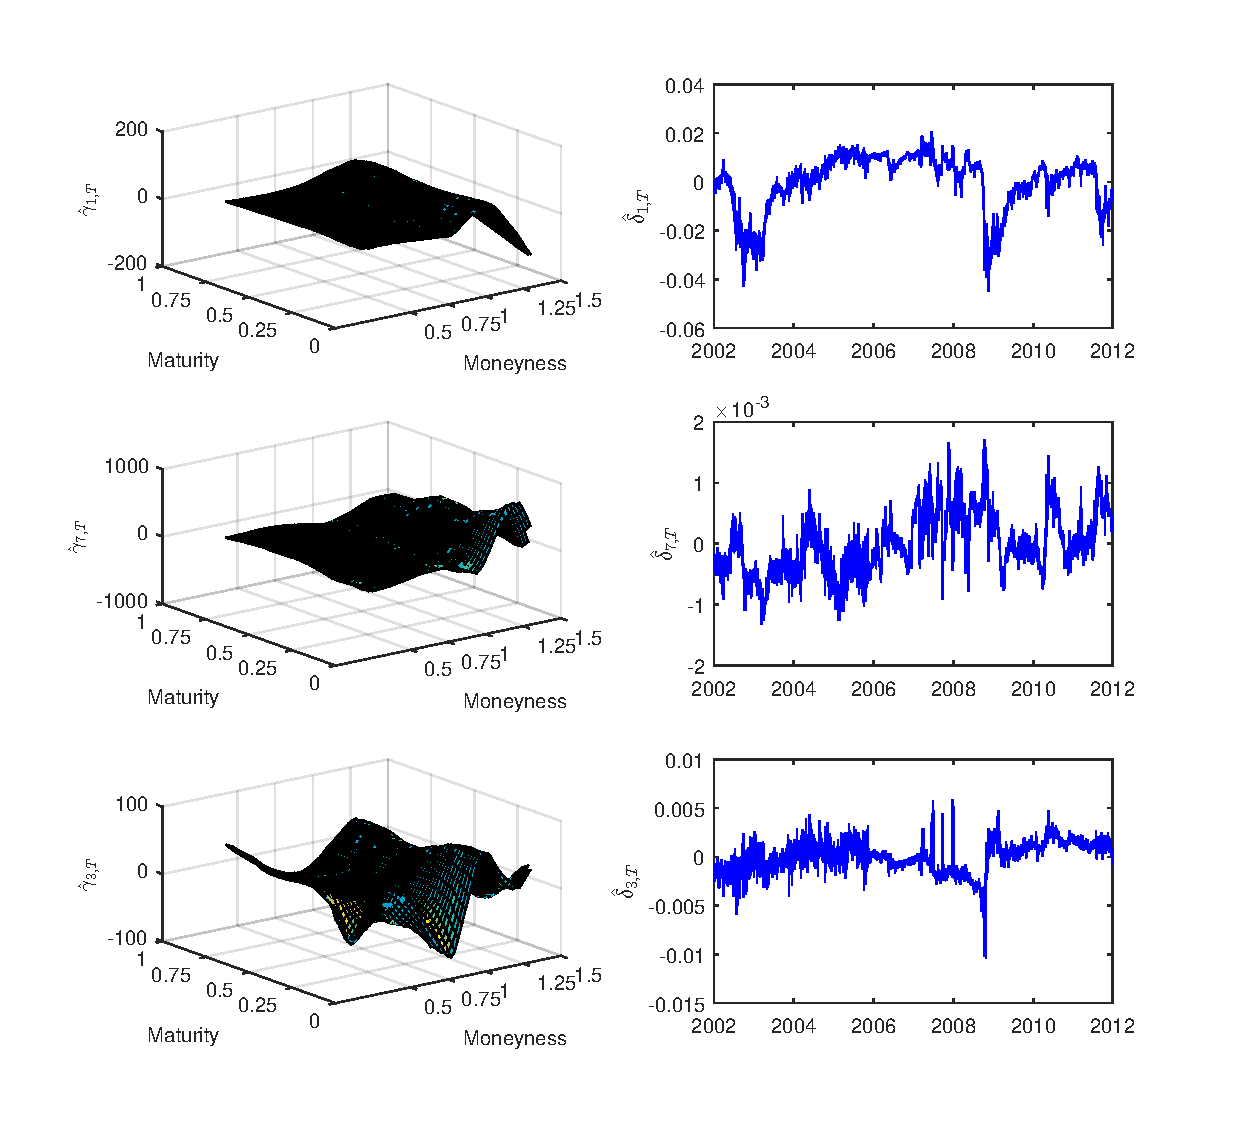
\includegraphics[width=1.0\textwidth]{figures/Nonorthogonalbasis20160521}
%\includegraphics[width=1.00\textwidth]{figures/Nonorthogonalbasis1} \\
%\includegraphics[width=1.00\textwidth]{figures/LoadingsFPCA1}
%\includegraphics[width=1.00\textwidth]{figures/Nonorthogonalbasis2}
%\caption{\label{second_comp} Left: Call options on the expiration day. Right: Second non-orthogonal component $\hat{\gamma}_{2,T}$}
\caption{\label{nonort} Estimated components $\hat{\gamma}^{(d)}_{1,T}$, $\hat{\gamma}^{(d)}_{3,T}$ and $\hat{\gamma}^{(d)}_{7,T}$ and their loadings obtained by the decomposition of the dual covariance matrix $\hat{M}^{(0)}$}%, in decreasing order of explained variance from up to bottom}
\footnotesize \href{https://github.com/QuantLet/FPCA/tree/master/FPCAcomponents}{\color{black}\quantnet FPCAcomponents}
\end{center}
\end{figure}


%The other three most important estimated non-orthogonal components
The estimated components $\hat{\gamma}^{(d)}_{1,T}$, $\hat{\gamma}^{(d)}_{3,T}$ and $\hat{\gamma}^{(d)}_{7,T}$ together with their loadings are displayed in Figure \ref{nonort}. %, in order of their explained variance, see equation (\ref{varnno}). %To enable comparison, they have been multiplied by the standard deviation of the corresponding loadings. %Scaled $\hat{\gamma}_{1,T}$ and $\hat{\gamma}_{3,T}$ are similar in hight but the peak of
%The first component is aligned with the mean, and has positive values around the peak and negative around the tails. The other two components resemble the orthogonal components in the simulation study. Some differences stem from the fact that the empirical SPD are left-skewed, compared to the right-skewed mixtures of log-normals. %This also explains a lower first 'valley' in the second component. Another difference in the tail behavior of the first two components - steep slope and negative values - might be due to interpolation errors in the regions with few observations. Other than that, the components provide a similar interpretation to those in the simulation study.
They describe three types of asymmetry present in the dynamics of the SPDs. %Their interpretation, is linked to the shape of the empirical mean of the SPD, which is negatively skewed. %which has a long tail on the left side of the peak. %A negative skew reflects the market expectation that the future stock index will be above its forward value. While negative skewness risk can bear excess returns, during periods of economic downturn, the investors prefer positively skewed distributions.
The first component, is similar in shape to the empirical mean of the SPD. It has a long left tail, specific to the negatively skewed densities and a peak located at a value of moneyness slightly above one. For positive levels of the loadings, this component increases the mass of SPD around the mode and decreases the values in the tails. We find that this component is related to the time-varying volatility of the index returns. %It takes positive values around the peak and negative around the tails and is closely related to the volatility of the SPD dynamics. An increase in the loadings of this component decreases the volatility of SPD.
The next component, $\hat{\gamma}^{(d)}_{3,T}$ has a 'valley-hill' pattern, which shifts mass around the central region of the density. %It also influences the density far left tail.
A positive shock in the direction of this components increases the negative skewness, and a large negative shock can reverse the sign of the SPD skewness. This component is interpreted as a skewness factor. The last component, $\hat{\gamma}^{(d)}_{7,T}$ takes negative values in the left tail and displays a prominent positive valued peak at the right of the mode of the empirical SPD mean. %This component emphasized the dynamics of negative skewness and induces changes in the kurtosis of the density as well.
This component represents a tail factor, and we show that its loading can be interpreted as the volatility of volatility index. %It also impacts the SPD skewness.% mass around the mean of the distribution and can
%We interpret it as the negative skewness factor. %The third component has a more symmetric 'valley-hill' pattern, which shifts mass around the central region of the density. It also influences the density far left tail. A positive shock in the direction of this components increases the negative skewness, while a large enough negative shock will render the SPD positively skew. This component is interpreted as the sign of skewness factor.  % and influences also particularly the the to the tails at the expense of the regions in between in a disproportionate fashion. The variations are larger in amplitude in the left half of the distribution. This component is interpreted as a kurtosis factor.
%crosses zero four times (for fix maturity). It influences the kurtosis of the density: it %simulated that of the second component is shifted to the right and is steeper for maturities of less than three months - options with shorter maturities are supposed to react stronger to changes. Both their right tails are negative, possibly due to the smoothing errors outside the observable data region.


%A negative skewness of the SPD reflects the market expectation that the future stock index will be above its forward value. Usually, the negative skew increases together with the implied volatility. While negative skewness risk can bear excess returns, during periods of economic downturn, the investors prefer positively skewed distributions. This can be seen when looking at the large negative values of $\hat{\delta}_{3,T}$ which, in effect, shift the SPD mass from the positive to the negative side of the distribution, in conformity with an increase in the risk aversion of investors.

%The loadings $\hat{\delta}_{1,T}$, $\hat{\delta}_{7,T}$  and $\hat{\delta}_{3,T}$ display a time-varying volatility regime, which divide the sample in three sub-periods that may reflect the impact of the global environment on the option prices. The end of 2005 marks the decline in the global liquidity and the end of 2008 is the conjectured conclusion of the global financial crises. Formal statistical tests for the equality of the loadings variance within the three subperiods can be run for a more thorough analysis. This can possibly unveil interesting economic questions, which will have to be left for further research. %We do not follow up on these observations because, as we show in the following, this variation is not longer present after orthogonalizing the loadings. %  \color{red}Changes in the mixture's distribution? We can interpret these as possibly changes in the mean function of the call prices or changes in the underlaying components Irina cite paper\color{black}. We will look at this issue in our following analysis. We will briefly return to them when discussing the connection between the SPDs and VDAX, in section \ref{?}.
%Therefore, we delete components two and four to represent the dynamics of $\bar{C}^{((2,0))}$ in terms of the orthogonal components, see figure \ref{rez}.


%From the simulation study we know that the variation explained by the third orthogonal component for density mixtures is significantly smaller than those of the first two. This is likely to translate in relatively small variations of the call prices as well. However, this component is important for explaining the moments of the DAX returns, for hedging or pricing purposes. We are therefore interested to identify it from the noisy data. Based on the criteria for the choice of number of factors, a less conservative choice for a proper truncation of the model is $L=9$.

% If we exclude this period from our sample the forth component is not 'loosing' its importance as well.
 %Here, it proves useful to have some prior knowledge about the shape of the components we expect to identify empirically.
%When investigating the variation of densities, one must be cautions because - as seem in the simulation study - the variation explained by further components is relatively small compared to the first two ones. Hence, without a proper ``shape marker/identifier'' one might easily confound them with noise.
 %It proved useful to have some prior knowledge about the shape of the orthogonal components in order to choose a proper truncation of the model.
%First, we look at the shape of the components and the dynamics of their corresponding loadings. Components $\hat{\gamma}_{4,T}$ and $\hat{\gamma}_{7,T}$ are similar in shape to $\hat{\gamma}_{2,T}$ and their loadings suffer from the same problem as $\hat{\delta}_{2,T}$. We therefore remove them from the candidate factors.

%\begin{figure}[ht]
%\begin{center}
%\includegraphics[width=1.00\textwidth]{figures/Rotatedorthogonal1} \\
%\includegraphics[width=1.00\textwidth]{figures/Rotatedorthogonal2}
%\includegraphics[width=1.00\textwidth]{figures/Orthogonalbasis1mew}\\
%\includegraphics[width=1.00\textwidth]{figures/Orthogonalbasis2mew}
%\caption{\label{second_comp} Left: Call options on the expiration day. Right: Second non-orthogonal component $\hat{\gamma}_{2,T}$}
%\caption{\label{nonortrot} First four rotated orthogonal components when including  $\hat{\gamma}_{1,T}$, $\hat{\gamma}_{2,T}$ and$\hat{\gamma}_{3,T}$}
%\end{center}
%\end{figure}

% The purely autoregressive model explains the dynamics of the risk-neutral implied moments rather well. \color{red} Adding exogenous variables to the vector autoregression does not improve the explanatory power of our model. \color{black}




%One-step ahead forecasting accuracy, measured as the RMSE of the in-sample forecasting errors imply that the first model is better in terms of prediction. These models can be used to investigate Granger causality relations between the loadings.



%The shape features of the three components from Figure (\ref{nonort}) and their ordering according to the explained variance are stable to orthogonalization, when we use the truncation choice  $\sum_{r\in \{1,3,7\}}\hat{\delta}_{r,T}\hat{\gamma}_{r,T}$.
The functional principal components of the reduced model $\sum_{r\in \{1,3,7\}}\hat{\delta}_{r,T}\hat{\gamma}^{(d)}_{r,T}$ resemble closely the three components displayed in Figure \ref{nonort}. % is possibly introduced through the dynamics of the interest rate term structure
%This means that if we ignore the term effect, which expresses the asymmetric reaction intensity to changes in the economic environment between the short and long term term option prices, the first three orthogonal components of the reduced model can still be interpreted as volatility, skewness and kurtosis factors. To avoid the burden of introducing additional notation we use non-orthogonal estimates in our further analysis.
Further analysis shows that when including any additional component to the reduced representation, the shape of the orthogonal basis changes to some extent. The loadings of all orthogonalized components become 'contaminated' with jumps. %Therefore, we use only three basis to describe the dynamics of SPDs % if the term structure effect of the SPDs is not considered. Variations of SPD in the maturity dimension introduces additional components, which are required to describe the asymmetric SPD changes for short and long maturities, similarly to the main modes of variation in the reduced model. %to reflect the uneven changes introduced by the term structure variation. %around the mean, skewness and kurtosis.
Moreover, all the loadings estimated by decomposing $\hat{M}^{(d)}$, for $d=(2,0)^{\top}$ feature the jump-behavior outlined above, between mid-February 2007 and mid-September 2008. For those reasons, $\hat{M}^{(0)}$ decomposition enables a better interpretation of the components, by separating the continuous and discontinuous sources of variation in the SPDs.


%Before proceeding further, we
We show next that the first estimated component $\hat{\gamma}_{1,T}^{(d)}$ is related to the expected variance under a risk neutral measure $Q$, which admits the density $q$.
Under this measure, the prices are martingales. Equations \eqref{der2} and \eqref{q091} yield

\begin{equation} \label{irapp}
%\begin{split}
\frac{{\EE}_{i}^{Q}\left(s_{i+\tau}/F_{i}\right)}{\exp(r_{i\tau}\tau)}=%&\int_{0}^{\infty}mq_i(m,\tau)dm\\
\int_{0}^{\infty}m\tilde{q}(m,\tau)dm+\sum_{r=1}^\infty \delta_{ir} \int_{0}^{\infty}m\gamma^{(d)}_r(m,\tau)dm=1,
%\end{split}
\end{equation}
%${\EE}_{i}^{Q}\left(s_{i+\tau}/F_{i}\right)=\int_{0}^{\infty}mq_i(m,\tau)dm=1$. Similarly, ${\var}_{i}^{Q}\left(s_{i+\tau}/F_{i}\right)=\int_{0}^{\infty}m^2q_i(m,\tau)dm-1$, where $F_{i\tau}=s_i\exp(r_{i\tau}\tau)$.
%${\EE}_{i}^{Q}\left(s_{i+\tau}\right)=\exp(-r_{i\tau}\tau)\int_{0}^{\infty}s_{\tau}q_i(s_{\tau},\tau)ds_{\tau}$. Expressing this equation in terms of $m=s_{tau}$
%together with \eqref{der2} and the SPD mean $\bar{q}$ yield
% \begin{equation}\label{irapp}
%\int_{0}^{\infty}m\bar{q}(m,\tau)dm+\sum_{r=1}^\infty \delta_{ir} \int_{0}^{\infty}m\gamma^{(d)}_r(m,\tau)dm=1, %=\exp(r_{i\tau}\tau)
%\end{equation}
where $\tilde{q}$ is the population mean. The computation of the second moment gives%${\var}_{i}^{Q}\left(s_{i+\tau}/F_{i}\right)$ we get
 \begin{equation}\label{varapp}
\frac{{\var}_{i}^{Q}\left(s_{i+\tau}/s_i\right)}{\exp(r_{i\tau}\tau)^2}=\int_{0}^{\infty}m^2\tilde{q}(m,\tau)dm+\sum_{r=1}^\infty \delta_{ir} \int_{0}^{\infty}m^2\gamma^{(d)}_r(m,\tau)dm-1.%{\EE}_{i}^{Q}\left(s_{i+\tau}/s_i\right)^2.
\end{equation}
We consider the empirical version of Equation \eqref{varapp}, for $\tau=1$ month. %The estimates of $\tilde{q}$ and $\gamma^{(d)}$ can suffer of sever bias in the regions with a few observation.
Instead of computing the integrals, based on our estimates of $\tilde{q}$ and $\gamma^{(d)}$, we assume them to be unknown coefficients in a linear regression, in which the empirical loadings are used as explanatory variables of the real-data proxy for the standardized variance.
%Equation \eqref{varapp} indicates that there is a linear relationship between the loadings of the principal components $\gamma_r$ and the standardized second moment.
In the numerator, we use the squared VDAX index multiplied by $\tau$. This index is computed by Deutsche B{\"o}rse AG from the prices of call and put options and reflects market expectation under the risk neutral measure of the 30 day ahead square root implied variance for the DAX 30 log-returns, which is then annualized. \cite{Duan2010} show that squared volatility index is a good approximation of the expected risk-neutral volatility when the jumps are small. While the volatility index refers to the standard deviation of the log-returns under the risk neutral measure, it can still be used in the regression because the transformation $q(\log m,\tau)=mq(m,\tau)$ maintains the linear-relationship between the dependent and explanatory variables.
%For the left hand side of equation \eqref{varapp} we use the square of VDAX index in the numerator.
%shows that the variability of the standardized second moment of returns can be expressed in terms of the loadings.  on the can be used to select the most relevant components for the second moment of the SPD.
%Both equations suggest a linear relationship between the loadings of the principal components $\gamma_r$ and the moments of the state price density.
%We perform a stepwise standard linear regression %by increasing the number of explanatory variables by one at a time, and choosing that improves the most the
%and compare the goodness of fit in a $MSE$ sense, for $\tau=1$ month.
We find that the most important component in the regression is $\hat{\delta}_{1,T}$ (adjusted R-squared in the univariate regression is 93.97\%). When including $\hat{\delta}_{3,T}$ as an additional regressor, it increases the adjusted R-squared to 94.06\%, %absolute correlation 94.66\% absolute correlation. 3 improves marginally the R-squared to 94.06\%  -0.1675 correlation
while $\hat{\delta}_{7,T}$ has a negative marginal contribution to the goodness of fit of multivariate regression. %R-squared. %It is also worth mentioning that among the other component, the term structure component $\hat{\delta}_{2,T}$ also contribute to the explained variance. %the first seven loadings bring the

No skewness index is readily available, and we take a simple measure instead, Pearson's skewness coefficient. In terms of equations \eqref{irapp} and \eqref{varapp}, for a fixed maturity $\tau$, it is equal to
\begin{equation}\frac{1 -\operatorname{arg}\,\underset{m}{\operatorname{max}} \left\{q(m,\tau)\right\}}{\sqrt{{\var}_{i}^{Q}\left(s_{i+\tau}/s_i\right)}/\exp(r_{i\tau}\tau)}.
\end{equation}%This is a proxy measure for the slope of the implied volatility.
Since the first component $\hat{\gamma}_{1,T}^{(d)}$ is unimodal (as it is also $\hat{\gamma}_{2,T}^{(d)}$), the SPD mode is mostly affected by the loadings of the third component $\hat{\gamma}_{3,T}^{(d)}$ (and to some extend by those of the seventh component $\hat{\gamma}_{7,T}^{(d)}$). %The tail factor takes highest positive values during the financial crisis, consistent with fat tail, high-risk hypothesis.

%A negative skewness of the SPD reflects the market expectation that the future stock index will be above its forward value. Usually, the negative skewness increases together with the volatility. However, between 2006 to the end of 2008, for sustained increases in the SPD variance, $\hat{\delta}_{3,T}$ decreases substantially. While negative skewness risk can bear excess returns, during periods of economic downturn, the investors prefer positively skewed distributions. This is in line with the finding of \cite{Feunou2013} conditional skewness changes sign over time. We try to understand the sources of this behavior in our further analysis.


%The other components $\hat{\gamma}^{(d)}_{4,T}$, $\hat{\gamma}^{(d)}_{5,T}$, $\hat{\gamma}^{(d)}_{6,T}$ and $\hat{\gamma}^{(d)}_{8,T}$, whose loadings have similar jump-behavior, have similar shape features to the four components discussed so far: $\hat{\gamma}^{(d)}_{1,T}$, $\hat{\gamma}^{(d)}_{2,T}$, $\hat{\gamma}^{(d)}_{3,T}$ and $\hat{\gamma}_{7,T}$. Their loadings have ``jumps'' alike $\hat{\delta}_{2,T}$. We contend that they are related to the asymmetric behavior of the option prices along the maturity direction, i.e., the term structure effect of the SPDs.


%We verified this by varying the number of factors before orthogonalization. We found that the shape features of the first three orthogonalized components from is preserved, while their loadings display jumps, similarly to $\hat{\delta}^{(d)}_{2,T}$ if any of the other 'noisy' components are added, similarly to the loadings $\hat{\delta}^{(d)}_{r,T}$. In fact, shape-wise $\hat{\gamma}_{1,T}$, $\hat{\gamma}_{2,T}$ and$\hat{\gamma}_{3,T}$ correspond to the estimates $\hat{\varphi}_1^{(d)$, $\hat{\varphi}_2^{(d)$ and $\hat{\varphi}_1^{(d)$. The other three orthogonal basis obtained from the decomposition of $\hat{M}^{(d)}$, are also related to the behavior of short term maturities. For instance, $\hat{\gamma}_2^{(d)$, closely resemble $\hat{\varphi}_4^{(d)$. We posit that three basis are necessary to explain variation of the SPDs if the term effect is not considered. The term effect introduces additional components, that decompose the term variation in variation around the mean, skewness and kurtosis. %The correlation structure between the loadings $\hat{\delta}_{r,T}$ and $\hat{\delta}^{(d)}_{r,T}$ are showed in table \ref{????}.

%Further, we analyze our results in terms of the orthogonal components. This allows us to perform a direct comparison between the estimation of the SPD by the two methods we presented in the previous sections. %compare them with the alternative estimation method based on the decomposition of $\hat{M}^{(d)}$.
%For this, we rotate the remaining six components, by applying a projection $a$, such that: $\sum_{r\in \{1,3,5,6,8,9\}}\hat{\delta}_{r,T}\hat{\gamma}_{r,T}=\sum_{r=1}^6a_r \tilde{\varphi}_r^{(d)}$, where $\tilde{\varphi}_r$ are the functional principal
%components for the reduced model and $a_r$ the corresponding loadings. By proceeding in  this way, the important commonalities in the nonorthogonal factors will be concentrated in even fewer components. %This also allows us to interpret our results in terms of components with known shape and also compare them with the alternative estimation method based on the decomposition of $\hat{M}^{(d)}$.
%The results are displayed in figure \ref{nonortrot}, for the first four orthogonalized components. The first three closely resemble the orthogonal components from our simulation study. One difference stems from the fact that the empirical SPD are left-skewed, compared to the right-skewed log-normals and their mixtures. This also explains a lower first 'valley' in the second component. Another difference in the tail behavior of the first two components - steep slope and negative values - might be due to interpolation errors in the regions with few observations. Other than that, the components provide a similar interpretation to those in the simulation study. They describe three type of asymmetries present in the dynamics of the SPDs. The first component that peaks at the same location as the mean curve, redistributes mass from the peak to the tails and can be related to the volatility dynamics. The second component, can be interpreted as influencing the skewness of the density: it adds mass to the central region and subtracts mass from the tails. The third component, shifts the density mass between the left and right sides and can be linked to the skewness factor. The corresponding loadings $a_r$ are no longer appear to be heteroskedastic. We will return to the analysis of their dynamics in the next subsection. (short characterization of the dynamics that anticipate findings in the next section).


%Two orthonormal components explain almost the entire variance of the reduced model, namely $99.74\%$ and $0.26\%$ respectively. 3rd??? The role played by the two components in explaining the variation of the SPD must be interpreted with caution, as changes in different regions of the underlying density may signal changes in the characteristics of underlying economic risks and market reaction to them, as well as impact the prices of the contingent clams on the underlying asset in a disproportionate fashion. For instance, it is well known that the deformation of the tail distribution conveys important information about the probability of extreme events that affect portfolio performance and hedging decisions. For the European options, small changes in the small probabilities can affect substantially the prices of far out of the money (OTM) options. Our further ananlysis suggests that both components are essential in undertanding the dynamics of SPD. Pricing of OTM Puts and Calls - asymmetris in the

%The second orthonormal component presents a positive peak situated around the peak of the mean. The right tail displays more negative values whereas the values of the component in the left tail fluctuate around zero negative. A positive shock in the direction of this component increases the peakness of SDP over the mean and decreases the mass of the distribution in the tails, in particular in the right one.

%\color{red}How do the factors influence the option prices?\color{black} Changes in the shape of the SPD translate to changes in the option prices. Whenever the probability mass for certain values of moneyness increases it will result in higher weights associated to the payoffs of the option in that particular states. For instance, a positive shock in both components will result in more expensive medium range OTM and cheaper far OTM calls. Conversely, a negative shock will make the prices of both far OTM put and call options increase while the prices of medium range OTM calls will decrease. This behavior can be related to the hedging behavior on the option market, see the discussions in \cite{Bollen:04}, \cite{Constantinides:11} and \cite{Kra:15}. % explain this behavior by  they don't like uncertainty.



%that including additional components preservesthe explained variance increases with each with each component that we include in the reduced model.


%We verified the consistence of our results by varying the number of factors before orthogonalization. We started by including only two components, $\hat{\gamma}_{1,T}$ and $\hat{\gamma}_{3,T}$, and investigated the principal components and their loadings for the reduced model. We repeated the procedure by increasing the number of components one at a time. We found that including additional components preserves the features of the first two orthogonalized components from figure \ref{nonortrot}, while the explained variance increases with each with each component that we include in the reduced model. The shape of the third component becomes stable once we add $\hat{\gamma}_{6,T}$. If we include only three components ($\hat{\gamma}_{5,T}$) then the third principal component is similar in shape to the fourth component in figure \ref{nonortrot}. Finally, deciding how large $L_d$ should be taken in practice, i.e. how many principal components, is both a matter of interpretation ability in terms of the shape of the components and of their loadings to capture as much variance in the data as possible, and adequately describe the dynamics of the underlying high-dimensional curves by correctly eliminating the noise terms.  \color{red} approximate factor model ???\color{black}



%The loadings are strongly correlated. This means that a factor model may be appropriate.
%This observation is supported by the results from the decomposition of $\hat{M}^{(d)}$, for $d=(2,0)$. Most of the criteria for choosing $L_d$ by this approach suggest six components.

%The optimal choice for $L_d$ from the $CP^{(d)}$ criteria gives at least six components, while both the eigenvalue ratio and $IC^{(d)}$ give six components. If we look at Figure \ref{ort}, we notice that there are three pairs of similarly-shaped components: the first pair $\hat{\varphi}^{(d)}_{1,T}$ and $\hat{\varphi}^{(d)}_{2,T}$ relate mainly to changes in the volatility, the second pair $\hat{\varphi}^{(d)}_{3,T}$ and $\hat{\varphi}^{(d)}_{5,T}$ looks similar to $\hat{\gamma}^{(d)}_{2,T}$, while the third pair $\hat{\varphi}^{(d)}_{4,T}$ and $\hat{\varphi}^{(d)}_{6,T}$ is similarly shaped to the negative skewness component from the previous decomposition. %The first pair relate to the volatility, the second pair appear similar to $\hat{\gamma}^{(d)}_{2,T}$, while the third pair is similar to the negative skewness factor. %However, this interpretation is not straight-forward and investigating additional components might shed additional light into this issue.


%We plot as well $\hat{\varphi}^{(d)}_{7,T}$ and $\hat{\varphi}^{(d)}_{8,T}$, which can be interpreted as skewness sign factors. These components are quite small and some of the criteria for the selection of the number of factors based on this approach might be overlooking his importance. Except for the first components estimated by each method, the loadings corresponding to $\hat{\varphi}^{(d)}$ and $\hat{\gamma}^{(d)}$ display only mild or low correlations. Therefore, a direct correspondence between the components is not straight forward. However, an approximate factor model is possible to hold for these data. As regards the 'duplicity' of the components, our results are most likely a manifestation of the SPD term effect, e.g. options with various maturities react differently to changes in the economic conditions. Accordingly, two factors in the term structure dynamics imply that two sets of components are required to explain the SPD implied expectations of long and short-run moments. This assumption is supported by looking particularly at the shape of the first pair, where the first component is relatively flat and describes reactions in the SPDs for longer horizons and the second component is steeper and describes reactions in the SPDs for short maturities.%.  we contend that the two sets of components describe reactions in the SPDs for long and short maturities. %as clear as in the case of $\hat{\gamma}^{(d)}_{r,T}$s.
%Not displayed here, all the loadings of the estimated components by decomposing $\hat{M}^{(d)}$ display the jump-behavior we described before between mid-February 2007 and mid-September 2008. In that sense, the previous approach seems to provide more accurate estimates that allow for a better interpretation of the results. %These results occur because the extrapolating error is worse for the second derivative. They are, however, stable in terms of the volatility of the loadings.
%Approximate factor model might be possible if we look at figure \ref{ort}.

%The estimated correlations between $\hat{\delta}_{r,T}$ and $\hat{\delta}^{(d)}_{r,T}$ displayed in table \ref{corrt} show a strong correlation only between the loadings of the first components estimated by each method, while the other correlations are quite small. No significant correlations are obtained after applying FPCA to the reduced model either. (Try 8 components). The results are thus mixed, if a factor model is appropriate for our data. (Maximum correlation - maximize correlation between projections - Markus paper).

%From the simulation, we have learned that the variance explained by each additional components decreases 'more than' exponentially for each additional factor added, when there is no term structure effect. This is why, when decomposing the variance explained ... 1.2550     0.0025      0.0001 multiplied by a factor of $10^7$. In Table 2 - Reordered variance. How to decide on the number of factors?


%The optimal choice for $L_d$ from the $CP^{(d)}$ criteria gives $L_{\max}$ components for $L_{\max} \leq 5$, while $IC^{(d)}$ gives six components. The forth component is obviously related to the short-term maturity effect. In general, the loadings of all estimated components by decomposing $M^{(d)}$ display the jump-behavior we described before between mid-February 2007 and mid-September 2008. These results occur because the extrapolating error is worse for the second derivative.They are, however, stable in terms of the volatility of the loadings.

% for the dynamics of state price density surfaces.
%The first two estimated principal components are similar to the functional principal components of the reduced model, see figure \ref{ort}. The pairwise correlation between their corresponding loadings is also high, $corr(\hat{\delta}^{(d)}_{1,T},a_1)=0.75$ and $corr(\hat{\delta}^{(d)}_{2,T}a_2)=0.73$. The third component does not offer conclusive evidence either with respect to the shape or the correlation $corr(\hat{\delta}^{(d)}_{1,T},a_1)=-0.23$, which is relatively small. The forth component is obviously related to the short-term maturity effect. In general, the loadings of all estimated components by decomposing $M^{(d)}$ display the jump-behavior we described before between mid-February 2007 and mid-September 2008. %Further components are also relatively smooth compared to $\tilde{\phi}_4^{(d)}$ and they seem also affected by the small-maturities effect.
%These results occur because the extrapolating error is worse for the second derivative. % it might be that the second derivative amplifies the noise. One problem that occurs when taking derivatives is
%They are, however, stable in terms of the volatility of the loadings.
%A factor model with two components based on equation
%we choose the number of factors to be = to the largest variance before the reordering % $I(\alpha)$
\subsubsection{Dynamic analysis of the loadings } \label{dynamic} In this section, we investigate the dynamics of the loadings in the reduced model. The partial autocorrelation function of all three time series display a salient spike at the first lag. This suggests that an autoregressive or perhaps an integrated model of order one might be appropriate to represent their dynamics. Their serial autocorrelations decay slowly, similarly to the integrated processes that feature a stochastic trend. Unit root and stationarity test results (not reported here) are ambiguous. When the null hypothesis assumes the existence of a unit root (augmented Dickey-Fuller unit-root test, Phillips-Perron test, variance-ratio test for random walk) the tests reject the null, while stationary tests that have the unit root hypothesis as an alternative (KPSS test, Leybourne-McCabe stationarity test) favor the alternative. Based on these results, we further investigate if the loadings are fractionally integrated of order $\alpha\in (0,\,1)$, which is typical to long-memory processes. %This means that a current shock impacts their future levels over a long period and eventually dissipates. %Typically their autocorrelation function decays at a slower rate than exponential.
%Classical approach to detect the long-range dependence can be found in \cite{Hurst1951}, \cite{Mandelbrot1972}, which employ the R/S statistic. Applying \cite{Lo1991} modified the $R/S$ statistic, which corrects for the short-term autocorrelation, we obtain $N^{1/2}R^{1}_9 = 5.1582$, $N^{1/2}R^{3}_9 = 5.1582$, $N^{1/2}R^{7}_9 = 5.1582$, with $95\%$ confidence interval $(0,809,$  $1,862)$.
%To detect the long-range dependence in each series, we or $R/S$
%  He modifies the R/S statistic to account for the effect of short-range dependence by applying a �Newey-West� correction (using a Bartlett window) to derive a consistent estimate of the long-range variance of the timeseries. For maxlag> 0, the denominator of the statistic is computed as the Newey-West estimate of the long run variance of the series. For maxlag> 0, the denominator of the statistic is computed as the Newey-West estimate of the long run variance of the series.
We employ \cite{Lo1991}'s modified $R/\tilde{S}$ (range over standard deviation) rescaled statistic $\tilde{V}_N$, for a time series sample of $N$ observations. %,  which reduces the bias introduced by the short-term dependencies.
The denominator of the statistic is computed as the square root of \cite{Newey1987} estimator of the long run variance of the time series. %uses the rescaling factor $\tilde{S}$ to remove
%We consider
For a maximum lag $q=[N^{1/4}]=9$, we obtain $\tilde{V}_{N,1}(9) = 5.1582$, $\tilde{V}_{N,3}(9) = 4.5248$ and $\tilde{V}_{N,7}(9) = 4.9893$, with $95\%$ confidence interval $(0,809,$  $1,862)$. % We obtain $N^{1/2}R^{1}_9 = 5.1582$, $N^{1/2}R^{3}_9 = 4.5248$ and $N^{1/2}R^{7}_9 = 4.9893$, with $95\%$ confidence interval $(0,809,$  $1,862)$.
The tests reject the hypothesis that loadings have short-memory. We also apply \cite{Geweke1983} log-periodogram regression model to estimate the Hurst exponent. The estimates are $H_{1}^{GPH}=1.3736$, $H_{3}^{GPH}= 1.1761$ and $H_{7}^{GPH}= 1.1433$ for the cutoff $[N^{1/2}] = 50$. The $95\%$ confidence interval $(0.2981,$  $0.7019)$ for the the GPH estimator is calculated using a bootstrapping procedure proposed by \cite{Weron2002}. These estimates imply an order of integration $\hat{\alpha}_r^{GPH}=H_{r}^{GPH}-0.5,\, r=1,3,7$. It is known that in the presence of large autoregressive or moving average terms, $\hat{\alpha}_r^{GPH}$ is biased upwards. In general, these models are nontrivial to estimate by other methods. %$\alpha$ is computationally difficult %if one uses a misspecified fractionally integrated discrete time white noise process.
Furthermore, fractionally integrated processes lack a clear economic interpretation. Therefore, instead of including a large number of autoregressive terms we use a parsimonious AR(1) model with time varying coefficients to approximate the long memory process.
%we approximate the long memory process by an autoregressive model. %Furthermore, the real %The results confirms the previous evidence that the loadings have long memory. %(The estimate of d, 0.404, is far from zero, indicating the presence of long-range dependence). It is known that for large positive AR or MA roots the estimator of d is seriously biased upwards. Attention has therefore focused on joint MLE of all parameters in the ARFIMA(p; d; q) models. In practice, these models are hard to estimate fractionally integrated models are nontrivial to estimate and not easily extendible to multivariate processes and lack clear economic interpretation, Comte and Renault (1998).
This is appropriate also for $\alpha \in (1/2,\,1)$, when the loadings are not stationary, see \cite{Comte1998}.
%For $\alpha \in (1/2,\,1)$, the loadings are not stationary but can be approximated by an autoregressive model, see \cite{Comte1998}. %Therefore, we use a moving window approach to model the univariate processes as $AR(1)$ processes. (we compare the results with the VAR(1), $I(\alpha)$), Heterogeneous Autoregressive model (HAR), used to predict realized volatility. (Long memory a large number of autoregressive terms are required ... instead, short term characteristics give more weight ... additional flexibility by letting the parameters of an AR(1) model and the error variance or covariance matrix to be time varying)


%This implies an estimated order of integration $\hat{d}^r=H^{r}_{GPH}-0.5$. The simplest long-memory formulation is an autoregressive fractionally integrated moving-average model ARFIMA(0, $\hat{d}^r, 0)$. Additional AR and MA terms can be estimated but the estimation is nontrivial. For the purpose of the current work we do not pursue this endeavor.

%In addition, the time series of loadings are heteroskedastic (tests). Long memory processes observed at discrete points in time can be represented as discretized mean-reverting processes, see \cite{Comte1996} and {Comte1998}.


We consider the following law of motion for the loadings
\begin{equation}\label{ar_eq}
 \hat{\delta}_{ir,T}=b_r\hat{\delta}_{i-1r,T}+e_{ir}, \quad \var(e_{ir})=\sigma_{er}^2,
\end{equation}
where $b_r$ is the autoregressive coefficient, $r=1,\,3,\,7$. We reestimate equation \eqref{ar_eq} daily on a moving window of 250 observation using OLS. This adaptive estimation procedure helps detect the possible sources of non-stationarity in the estimated loadings, by allowing the autoregressive coefficient and the error variance to vary over time. %It also provides a parsimonious representation, with
%In order to account for the possible presence of serial correlation in the data, the Newey-West covariance correction for serial correlation is employed. We also report the results for the AR models estimated over the entire sample \color{red}(MSE-I($\alpha$)) \color{black}. Table (\ref{tab:MW:AR}) reports the estimation results for the three series.

\begin{figure}
\begin{center}
%\includegraphics[width=1.00\textwidth]{figures/corr_load}
\includegraphics[width=1.00\textwidth]{figures/AR_corr}
%\caption{\label{window}  250 days moving window correlation coefficient for the first-difference of the loadings and volatility of implied volatility index}
\caption{\label{window} Time varying autoregressive coefficients, standard deviations of the error, pairwise error correlations from fitting a univariate AR(1) model to each loading; and time varying standard deviation of the VDAX volatility index estimated daily with a moving window of 250 observations}
\footnotesize \href{https://github.com/QuantLet/FPCA/tree/master/FPCAloadings}{\color{black}\quantnet FPCAloadings }
\end{center}
\end{figure}




The upper left panel of Figure \ref{window} displays the estimated autoregressive coefficients. $\hat{\delta}_{1,T}$ is very persistent ($\hat{b}_1$ is close to one) for most of the time, except 2004. Interestingly, $\hat{b}_3$ is relatively small between 2003-2006 and increases significantly thereafter, suggesting a possible regime shift. $\hat{b}_7$ is relatively high and its variation seems sensitive to the changes in the other two parameters.

In addition, we compute the time-varying correlations between the error terms in each loading equation. These correspond to the non-diagonal entries of the empirical error covariance matrix for a vector autoregressive model of order one VAR(1) fitted to the loadings, with diagonal autoregressive coefficient matrix. The two lower panels of Figure \ref{window} illustrate the results. The error correlation of the skewness with the volatility and the tail factor loadings move closely together, suggesting a strong relationship between the volatility and the tail factors. We focus on $corr(\hat{e}_1,\hat{e}_3)$, which describes the dynamic relationship between the changes in SDP volatility and skewness. Most of the time, the plotted correlation is negative, meaning that positive changes in the SPD variance are associated on average with increases in the negative skewness. %A negative skew reflects the market expectation that the future stock index will be above its forward value.
The negative correlation between an asset return and its changes of volatility
is generally known as the leverage effect. %In general, it refers to the negative correlation between an asset return and its changes of volatility.
%positive shocks to the volatility equation are associated on average with positive shocks to skewness equation. . The reversion in the correlation
The correlation reverses sign and becomes positive between 2007-2009. This means that when volatility increases, there is a change in the concentration mass in the left side of the density, in the area of medium-ranged negative returns. %This has as effect an overall flattening of the left tail. % and results in more expensive OTM puts and relatively cheaper deep OTM options.
We identify this behavior with the implied volatility skew puzzle, as documented by \cite{Constantinides2015}. The authors rationalize this behavior through the reduction in put option supply from credit-constrained market makers together with an increase in the demand for OTM puts required for hedging purposed, see net buying pressure in \cite{Bollen2004}, \cite{Garleanu2009}.% Our findings according to which the difference between the prices of OTM and ATM put options decreases during the financial crisis, is consistent with their observation that the implied volatility skew declines. giving rise to more expensive OTM puts and relatively cheaper deep OTM options.
%Similarly, we can characterized the relationship between ...

%The tail factor takes highest positive values during the financial crisis, consistent with fat tail, high-risk hypothesis.

%A negative skewness of the SPD reflects the market expectation that the future stock index will be above its forward value. Usually, the negative skewness increases together with the volatility. However, between 2006 to the end of 2008, for sustained increases in the SPD variance, $\hat{\delta}_{3,T}$ decreases substantially. While negative skewness risk can bear excess returns, during periods of economic downturn, the investors prefer positively skewed distributions. This is in line with the finding of \cite{Feunou2013} conditional skewness changes sign over time. We try to understand the sources of this behavior in our further analysis.
% a concentration of mass toward the left and a long tail to the right

%This phenomenon is explained in the empirical financial literature through the net buying pressure of index options (\cite{Bollen2004}, \cite{Garleanu2009}). %Overall, $\hat{\delta}_{7,T}$ is linked to sudden and short-term changes in volatility.

%The overall flattening of the left tail together with volatility increases is a manifestation of the implied volatility skew puzzle, as documented by \cite{Constantinides2015}. The authors explain it through the reduction in supply of put options from credit-constrained market makers when the demand for puts increases. Our findings according to which the difference between the prices of OTM and ATM put options decreases during the financial crisis, is consistent with their observation that the implied volatility skew declines. giving rise to more expensive OTM puts and relatively cheaper deep OTM options.


Typically, the error correlation $corr( \hat{e}_{1} , \hat{e}_{7})$ is negative. Its magnitude decreases and reaches values close to zero in 2009. In the lower right panel of Figure \ref{window}, we also plot the 250-observation standard deviation $\hat{\sigma}_{IV}$ of the VDAX implied volatility index. The two time-series are strongly correlated (the correlation coefficient is 90.78\% ). % correlation with S&P500 index option volatility,  )
This suggests that the tail component can be interpreted as the volatility of volatility risk factor. Similar interpretations were proposed in \cite{Du2012}, \cite{Huang2014}  or \cite{Park2015}, who use different measures of the volatility-of-volatility implied by VIX (the implied volatility index of the S\&P 500) as a tail risk indicator. The tail factor takes highest positive values during the financial crisis, consistent with fat tail and high risk hypothesis.

%In general, we obtain almost perfect correlations when the implied volatility index ( $\hat{\delta}_{1,T}$) is very small.

%Its correlation with delta d1 is negative for most of the time, except in 2009 when after a sudden increase and subsequent decrease in volatility d7 continue to decrease and become negative. This reverse reaction means that the OTM put options become more expensive as volatility increases.


%The error terms are strongly correlated (persistence) white noise tests show that are strongly.

To verify the stability of the results reported, we repeat the regression analysis by including a constant in equation \eqref{ar_eq}. The root mean square error does not decrease significantly. %, therefore, we report the results without the constant.
We also estimate the model by including the lagged values of the other two loadings as additional explanatory variables. Some of the estimated autoregressive coefficients take value above one. Independently of these modeling choices, the estimated error covariances are very similar to those shown in Figure \ref{window}. These suggest that changes in the correlation sign for the levels is due to the error term correlation structure and not to changes in the lagged cross-term interactions.

% We also looked at the VAR models but the effect of the other loadings are significant ... do not improve the Mean square. or it improves it in only 50\% of the time. The parametrs dynamics and the correlations do not change signifficantly the findings reported in figure. Meaning that the correlatin structure in the error term is not due to past cross-term interactions.
%The analysis enables us to distinguish as well between the volatility induced skewness through the leverage effect and by the volatility of volatility induced skewness, \cite{Feunou2012}

Several stylized facts emerge from the moving window estimation of autoregressive models for the loadings that summarize the dynamics of SPDs. %analysis of functional components of SPDs and the
% model $AR(1)$ from equation \eqref{ar_eq} using a moving window illustrate
% The first factor when no jumps --- stochastic volatility model - the variance when no jumps are present.
%Dynamic estimation of $AR(1)$ model from equation \eqref{ar_eq} using a moving window suggests variation in both autoregressive coefficients and covariance structure. When the empirical errors are (almost) perfectly correlated, the innovations in the volatility, skewness and volatility of volatility dynamics can be interpreted as expression of the same factor. This occurs in our empirical analysis when SPD volatility is small.
When volatility is small, the innovations to the volatility, skewness and volatility of volatility loading equations are very strongly correlated. %Possibly, they can be interpreted as expression of the same factor.
When volatility increases, the correlation structure changes. In particular, the leverage parameter changes sign during the financial crises. By including volatility of volatility as an additional factor, see also \cite{Huang2014}, our study distinguishes between the volatility induced skewness through the leverage effect and by the volatility of volatility induced skewness, see also \cite{Feunou2012}. These findings may have important consequences for the formulation of stochastic volatility models for option pricing. The empirical evidence suggests that the option markets include sources of variation that may not be present in the underlying's dynamics, such as frictions between option demand for hedging purposes and credit constrains for refinancing. It may be possible to formulate a model in which the changes in error correlations modify endogenously, possibly by controlling for the credit availability on the market. %Based on our findings, we include the volatility of volatility as an additional factor, see also \cite{Huang2014}. The analysis enables us to distinguish as well between the volatility induced skewness through the leverage effect and by the volatility of volatility induced skewness, \cite{Feunou2012}. %\cite{Constantinides2015} explain this effect in an equilibrium model with credit constrained market makers and increasing demand for put options.
%So far, The empirical evidence suggests that the option markets include additional sources of variation that are not present in the underlying's dynamics, such as option demand for hedging purposes and credit availability for refinancing.
%\textbf{Forecast}

%Table 5 and Figure 9 report the results for out-of-sample forecasts of the realized volatility in which the models are reestimated daily on a moving window of 1000 observations




%Another way of analyzing the loading dynamics is to use a moving window.
%Examining closer the dynamic relation for the loadings first difference, represented in Figure \ref{window} through the 100-days moving window correlation coefficient, we see that for most of the times the volatility and negative skewness factors move together.
%oftentimes the above mentioned correlation is close to -1  and but its strength also weakens and is sometimes reversed.
%The correlation structures that involve $\hat{\delta}_{7,T}$  show that this component expresses reactions to sudden and shorter term changes in volatility.
%Oftentimes the correlation of their difference $corr=(\Delta \hat{\delta}_{i1} , \Delta \hat{\delta}_{i7})$ is close to $-1$ and its strength weakens and is sometimes reversed, in a strong connection to the movements of the volatility of implied volatility index ($Vol_{IV}$), computed as a 100-days moving window standard deviation of the daily implied volatility index. %Its correlation with delta d1 is negative for most of the time, except in 2009 when after a sudden increase and subsequent decrease in volatility d7 continue to decrease and become negative. This reverse reaction means that the OTM put options become more expensive as volatility increases.
%The reversion in the correlation sign following the financial crises means that the OTM put options become more expensive as volatility increases. This phenomenon is explained in the empirical financial literature through the net buying pressure of index options (\cite{Bollen2004}, \cite{Garleanu2009}). Overall, $\hat{\delta}_{7,T}$ is linked to sudden and short-term changes in volatility.


%A similar behavior can be induced by $\hat{\delta}_{3,T}$. From 2006 to the end of 2008, $\hat{\delta}_{3,T}$ decreases and becomes negative during the financial crisis.
 %, giving rise to more expensive OTM puts and relatively cheaper deep OTM options.
%This increase in the negative skewness  (and/or or less fat left tail)
%The overall flattening of the left tail together with volatility increases is a manifestation of the implied volatility skew puzzle, as documented by \cite{Constantinides2015}. The authors explain it through the reduction in supply of put options from credit-constrained market makers when the demand for puts increases. Our findings according to which the difference between the prices of OTM and ATM put options decreases during the financial crisis, is consistent with their observation that the implied volatility skew declines.

% implied volatility skew puzzle is that the difference between OTM
%d 7 ---- component expresses reactions to sudden and shorter term changes in volatility.

%The evidence shows that d3 and d7 can be seen as long and respectively short term reaction to changes in volatility and volatility of volatility.

%After sustained periods of increases in the implied volatility, particularly between 2006 to the end of 2008, $\hat{\delta}_{3,T}$ decreases substantially. A negative skewness of the SPD reflects the market expectation that the future stock index will be above its forward value. Usually, the negative skew increases together with the volatility. While negative skewness risk can bear excess returns, during periods of economic downturn, the investors prefer positively skewed distributions. This can be seen when looking at the large negative values of $\hat{\delta}_{3,T}$ which, in effect, shift the SPD mass from the positive to the negative side of the distribution, in conformity with an increase in the risk aversion of investors. We try to understand the sources of this changes in the analysis below.

%The VAR coefficients imply that negative shifts in the first component, consistent with an increase in implied volatility, or decrease in the negative skewness, through negative movement of $\hat{\delta}_{7}$. A decrease in the negative skewness, through negative movement of $\hat{\delta}_{7}$. In effect, the slope of the left side of the SPD decreases and the price of deep out-of-the-money (OTM) puts increases.
%For not too small moneyness levels, this means less probability mass in the left side of the SPD, which translate in cheaper out-of-the-money (OTM) puts. For deep OTM puts, positive movements of $\hat{\delta}_{i3}$ imply a fatter left tail and hence higher prices.


%after applying the fractionally-integrated filter to the original series. It is known that this two-type procedure may not deliver consistent estimators because $\hat{d}^r$ is biased upwards in the presence of large AR or MA roots of the lag polynomial. %It is known that for large positive AR or MA roots the estimator of $d^r$ is seriously biased upwards and joint estimation of all parameters in the ARFIMA models is recommended. In practice, these models are nontrivial to estimate and not easily extensible to multivariate processes and lack clear economic interpretation, Comte and Renault (1998).

%In order to assess the impact of the AR terms, which enables comparison between models we use this approach. We find that the methodology produces estimated models that performs well in describing the dynamics of the loadings in sample and produces better forecasts compared with the alternative models. %In addition, the estimated AR coefficients are small in magnitude
% However, these models are much better in representing the loading dynamics in terms of mean-squared value comparative to a simple autoregressive (AR) or vector autoregressive (VAR) model but comparable to a heterogenous moving average (HAR) model, see discussion below.

\section{Conclusions}\label{t5}

In this paper, we describe two methods for representing derivatives of multivariate curves using FPCA techniques. First, spectral decomposition is applied to the dual covariance matrix of derivatives. Secondly, the dual covariance of the original curves is considered, and derivatives are obtained by differentiation of the functional principal components of the covariance operator. Thus, the second approach expresses the dynamics of derivatives in terms of uncorrelated loadings but the basis functions are no longer orthonormal. % but can be projected in order to obtain orthonormal components in a reduced model for the derivatives, if a factor model is assumed.
We demonstrate that when an underlying factor model is assumed, estimating curve derivatives from observed discrete and noisy data using a low-dimensional representation, the second method performs better both asymptotically and in finite sample. %In the real data example we find that three components can explain most of the variability in the data. Additional factors describe the variation of the term structure of the SPD. %These offer a parallel interpretation to the decomposition of implied volatility surfaces.
%The empirical analysis provides new insights into the economics behind the option pricing, which suggest the need to reconsider the last generation of arbitrage-free models for option pricing, see representative \cite{Bates2006}. %: hedging demand for options, short-selling constrains of OTM puts with overpriced underlying, credit-constrains of the money-makers during economic downturns. % Hence, we believe that the third principal component is a novel way of thinking about the gamma hedging.
%Our results also show that the negative skew and variance are manifestations of the same underlying risk factor, with the causality direction going from negative skewness to volatility.
%Further findings suggest the effectiveness of using option-implied SPD components to forecast future returns or future realized volatility of the underlying asset.

In the empirical study, we show that the second method provides accurate results for understanding the time variability of implied SPDs.
We apply this analysis to DAX 30 index option data observed at daily frequency. %and interpret the estimation results in the context of risk neural arbitrage-free models.
Three main factors are identified, which could be linked to the diffusion processes of the stochastic volatility models.
The first factor is strongly connected to the risk-neutral variance, conditional upon that no jumps occur. The second factor is related to the time varying conditional skewness induced by the leverage effect. %Contrary to the prediction of the standard stochastic volatility models, `
We find that this component of negative skewness declines during the financial crises, possibly as a result of the credit crunch. % as a result which is in line with the flattening of implied volatility skew reported by \cite{Constantinides2015}. who explain this effect in a model with credit constrained market makers and increasing demand for put options.
Time-varying volatility of volatility constitutes an additional risk channel, which manifests as negative tail risk. Further factors are related to the term structure and jump component risk. %We find that options with shorter maturities react stronger to the occurrence of jumps in the underlying. In accordance to the predictions of the jumps diffusion processes, discontinuities in the stock index capture additional increases in the SPD volatility, the negative skewness and fatter tails.

%Understanding time variability of option prices in terms of the underlying probability density is important for asset pricing because it conveys information about all the sources of variability for the underlying process, as well as the frictions of the market on which options are traded.  The loadings are estimated from the spectral decomposition of the dual matrix of the sample covariance operator of smooth option price functions, while the factors are based on the second derivative of the functional principal components, using local polynomial estimators.

%\newpage
\section{Appendix}%
\subsection{Assumptions summary}
\label{assum}
%\begin{assumptions}
%Let $X$ be a centered smooth random function in $L^2([0,1]^g)$, where $g$ denotes the spatial dimension, with finite second moment $\int_{[0,1]^g} \EE\left[X(u)^2 \right]du < \infty$ for $u=(u_1, \ldots, u_g)^{\top}$and $\EE\left[X(t) \right] =0$ . %Here, we consider
%\end{assumptions}
%\begin{assumptions}
%$X$ is at least $m+1$ times total continuously differentiable where
%\begin{enumerate}
%	\item $m \geq \max \left(2\|d|,\sum_{l=1}^g d_l \right)$ if $M^{(d)}$ is used to derive the decomposition
%	\item $m \geq \|d|$ if $M^{(0)}$ if $M^{(0)}$ is used to derive the decomposition
%\end{enumerate}
%and all the partial derivatives are bounded by a constant $C<\infty$ such that $\underset{t}{\operatorname{sup}}\underset{k \in (\mathbb{N}\cap [0,m+1])^g}{\operatorname{sup}}\EE\left[X_i^{(k)}(t)\right]\leq C$.
%	\item For $x \in supp(f) $, $f(x)>0$
%\end{assumptions}
\begin{assumptions}
\label{A1}
$X_1,\dots,X_n$ are i.i.d. centered random functions which are a.s. $m$ times  continuously  differentiable. All corresponding partial derivatives possess finite fourth moments for all $t\in  [0,1]^g$.
\end{assumptions}
\begin{assumptions}
\label{A1.1}
Following model \eqref{basic} functions
are observed at a random grid $t_{i1},\dots,t_{iT_i}$, $t_{ij}\in [0,1]^g$ having a common bounded and continuously differentiable density $f$ with support $\supp(f)=[0,1]^g$ and the integrand $u \in \supp(f)$ and $\underset{u}{\operatorname{\inf}}  f(u)>0$. The random variables $t_{ij}$ and $X_i$ are independent.
\end{assumptions}
\begin{assumptions}
\label{A2}
$\EE(\varepsilon_{ik})=0$, $\var(\varepsilon_{ik})=\sigma_{i\varepsilon}^2>0$, $\EE\left[\varepsilon_{ik}^4\right]<D$ for some $D<\infty$ and all $i=1,\dots,N$, and
 $\varepsilon_{ik}$ are independent of $X_i$ and $t_{ij}$,   $\forall i,k,j$. %$\sigma_{\varepsilon,i}^{-l} \EE\left[\varepsilon_{ik}^l\right]<\infty, \; l=3,4 \; \forall i,k$.
\end{assumptions}
\begin{assumptions}
\label{A3}
Let $K_B(u)=\frac{1}{b_1 \times \dots \times b_g} K(u \circ b)$. $K$ is a product kernel based on symmetric univariate kernels. $B$ is a diagonal matrix with $b=(b_1,\dots,b_g)^{\top}$ at the diagonal. The kernel $K$ is bounded and has compact support on $[-1,1]^g$ such that for $u \in \mathbb{R}^g$ $\int u u^T K(u) du = \mu(K) I$ where $\mu(K)\neq 0$ is a scalar and $I$ is the $g \times g$ identity matrix. Conditions 2 and 3 from \cite{Masry96} are fulfilled.
\end{assumptions}
\begin{assumptions}
\label{A4}
$\rho- \sum_{l=1}^g d_l$ and $p -\sum_{l=1}^g d_l$ are odd.
\end{assumptions}
\begin{assumptions}
\label{A4.1} Estimators of the error variances satisfy
$|\hat{\sigma}_{i\varepsilon}^2-\sigma_{i\varepsilon}^2|=\mathcal{O}_P(T^{-1/2}) $
\end{assumptions}
\begin{assumptions}
\label{A5}
\begin{equation}\label{cc1}
\underset{r\in \mathbb{N}}{\operatorname{sup}} \; \underset{t \in [0,1]^g}{\operatorname{sup}} | \varphi^{(d)}_r(t)| < \infty \;,\; \underset{r\in \mathbb{N}}{\operatorname{\sup}} \; \underset{t \in [0,1]^g}{\operatorname{\sup}} | \gamma^{(d)}_r(t)| < \infty
\end{equation}
\begin{equation}\label{cc2}
\sum_{r=1}^\infty \sum_{s=1}^\infty \EE \left[\left(\delta^{(\nu)}_{ri}\right)^2 \left(\delta^{(\nu)}_{si}\right)^2 \right] < \infty \;,\; \sum_{q=1}^\infty \sum_{s=1}^\infty \EE \left[\left(\delta^{(\nu)}_{ri}\right)^2 \delta^{(\nu)}_{si} \delta^{(\nu)}_{qi}\right] < \infty, \; \ \nu=(0,d)
\end{equation}
For $\nu=(0,\dots,0)^\top$ as well as $\nu=d$. 
Recall that necessarily $\EE \left[(\delta^{(\nu)}_{ri})^2\right]=\lambda_r^{(\nu)}$, and hence $\delta^{(\nu)}_{ri}=0$ a.s. iff $\lambda_r=0$.
\end{assumptions}
\begin{assumptions}
\label{A6}
Let $\nu=(0,\dots,0)^\top$ and $\nu=d$. For any $r\in \mathbb{N}$ with $\lambda_r^{(\nu)}>0$ there exists 
some 
 $0<C_{1,r}<\infty$  such that
\begin{equation}
\label{eigeval}
%\begin{split}
\min_{s\in \mathbb{N}; s \neq r} |\lambda^{(\nu)}_r-\lambda^{(\nu)}_s|\geq C_{1,r}.
%\end{split}
\end{equation}
\end{assumptions}

\subsection{Proof of Proposition \ref{Mbias} }
\label{prooflemma}

The proposition is an immediate consequence of the following lemma.


\begin{lemma}
\label{lemint}
Under the assumption of Proposition \ref{Mbias} let
$T \rightarrow \infty$, $\max(b)^{\rho+1} b^{-\nu} \rightarrow 0$, $\frac{\log(T)}{T b_1\times\dots \times b_g} \rightarrow 0$, $T b_1 \times \dots \times b_g b^{4\nu}\rightarrow \infty$. Then %, given a set of $T$ observations $Y=\left\{Y(t_1),\ldots,Y(t_T)\right\}$ of variable $X$
\begin{equation}
\begin{split}
&{\EE}_{t,X} \left[\hat{M}^{(\nu)}_{ij}\right]- \int_{[0,1]^g} X_i^{(\nu)}(t)X_j^{(\nu)}(t) dt =\mathcal{O}_p \left(\max(b)^{\rho+1} b^{-\nu} + \frac{1}{T^{3/2} (b^{2\nu} b_1 \times \dots \times b_g)}  \right) \\
&\var_{t,X}(\hat{M}^{(\nu)}_{ij})=  \mathcal{O}_p\left( \frac{1}{T^2 b_1 \times \dots \times b_g  b^{4\nu}  }+ \frac{1}{T}\right),
\end{split}
\end{equation}
\label{lmeintres}
\end{lemma}
where ${\EE}_{t,X}$ denotes  conditional expectation and $\var_{t,X}$  conditional variance given
$t_{ik}$ and $X_i$ for $i=1,\dots,n$ and $k=1,\dots,T_i$.


\subsection{Proof of Lemma \ref{lemint} }

For the proof of the lemma we will concentrate on the diagonal entries $\hat{M}^{(\nu)}_{ii}$ which are slightly more difficult due to the necessity of a diagonal correction.
%\label{prooflemma}
\subsubsection{Univariate case (g=1) } In the following proof we use $d$ instead of $\nu$. As noted by \cite{Ruppert:94} equation (\ref{polyeqkern}) can be stated up to a vanishing constant using equivalent kernels. Equivalent kernels can be understand as an asymptotic version of $W^T_d$. Let $e_l$ be a vector of length $\rho$ with $1$ at the $l+1$ position and zero else. Then $W^T_d(t)$ evaluates the function at point $u$ and is defined as $(T b^{d+1}) ^{-1} e_d^T S_T(u)^{-1}(1,t,\dots, t^\rho)^T  K(t)$. $S_T(u)$ is a $\rho \times \rho$  matrix with entries $S_{T,k}(u)= (Tb)^{-1} \sum_{l=1}^{T} K\left( \frac{t_l-u}{b} \right) (\frac{t_l-u}{b})^k$  such that
\begin{equation}
\label{STMat}
S_T(u)=
\begin{pmatrix}
S_{T,0}(u)	& S_{T,1}(u)	& \dots	 & S_{T,\rho}(u)      \\
S_{T,1}(u)	& S_{T,2}(u) 	& \dots  & S_{T,\rho+1} 	  \\
\vdots	& \vdots 	& \ddots & \vdots \\
S_{T,\rho}(u)	& S_{T,\rho+1}(u)	& \dots	 & S_{T,2\rho}(u)
\end{pmatrix}.
\end{equation}
Accordingly
\begin{equation}
\begin{split}
\EE ( S_{T,k}(t_{ij}) ) =& (Tb)^{-1}  \int_0^1 \sum_{l=1}^{T} K\left( \frac{x-u}{b} \right) \left(\frac{x-u}{b} \right)^k f(x) dx \\
=& b^{-1}\int_u^{1+u}  K\left( \frac{x}{b} \right) \left(\frac{x}{b} \right)^k f(x) dx = \int_{ub^{-1}}^{(1+u)b^{-1}} K\left(t \right)  t^k f(tb) dt.
\end{split}
\end{equation}

Since $K(t)$ has compact support and is bounded, for a point at the left boundary with $c\geq 0$ $u$ is of the form $u=cb$ and at the right boundary $u=1-cb$ respectively. We define $S_{k,c}=\int_{-c}^\infty t^k K(t) dt$ and $S_{k,c}=\int_{-\infty}^c t^k K(t) dt$ respectively and for interior points $S_{k}=\int_{-\infty}^\infty t^k K(t) dt$. Further we construct the $p \times p$ Matrix corresponding to (\ref{STMat}) with
\begin{equation}
   S(u)=
   \begin{cases}
     S_c=(S_{j+l,c})_{0\leq j,l \leq\rho} 	&\text{, $u$ is a boundary point} \\
     S=(S_{j+l})_{0\leq j,l \leq\rho} 	&\text{, $u$ is an interior point}\\
   \end{cases} .
\end{equation}
 The equivalent kernel is then defined as $K_{d,\rho}^{u*}\left( t \right)  = e_d^T S(u)^{-1}(1,t,\dots, t^\rho)^T  K(t)$ and the estimator can be rewritten as
\begin{equation}\label{polyeqkernn}
\hat{X}^{(d)}_{i,b}(u)= d! \beta_{d}(u) = \frac{d!}{T_i f(u) b^{d+1}} \sum_{l=1}^{T_i} K^{u*}_{d,\rho}\left( \frac{ t_{il}-u }{b}    \right) Y(t_{l})\{ 1+ \smallO_P (1) \}.
\end{equation}
The only difference between $W^T_d$ and $K^{u*}_{d,\rho}$ is that $S_T(u)$ is been replaced by $f(u)S(u)$. Regarding \cite{Masry96} we can further state that with a bandwidth fulfilling $\frac{log(T)}{T b} \rightarrow 0$ we have
uniformly in $u \in [0,1]$ that $S_T(u)^{-1} \rightarrow \frac{S(u)^{-1}}{f(u)}$ almost surely as $T \rightarrow \infty$. We will drop the $u*$ index concerning the equivalent kernel from now on.

By construction, the equivalent kernel fulfills that using the Kronecker-Delta $\delta$
\begin{equation}
\label{kron}
\int u^k K_{d,\rho}^*\left( u \right) du  = \delta_{d,k} \; \; 0 \leq d , k \leq \rho. %\; \forall i=1,\dots g
\end{equation}
As mentioned by \cite{Fan1995}, the design of the kernel automatically adapts to the boundary which gives the same order of convergence for the interior and boundary points, see \cite{Ruppert:94}. The estimator can be rewritten as
\begin{equation}
\begin{split}
&\int d!^2  \sum_{j=1}^{T_i} \sum_{l=1}^{T_i} W_d^T\left(\frac{t_{ij}-u}{b}\right)  W_d^T\left(\frac{t_{il}-u}{b} \right) Y_i(t_{il}) Y_i(t_{ij}) du \\
=& \int \frac{d!^2}{T_i^2 f(u)^2 b^{2d+2}} \sum_{l=1}^{T_i}  \sum_{j=1}^{T_i} K_{d,\rho}^*\left(\frac{t_{ij}-u}{b}\right) K_{d,\rho}^*\left(\frac{t_{il}-u}{b} \right) Y_i(t_{il})Y_i(t_{ij})\{ 1+ \smallO_P (1) \} du.
\end{split}
\end{equation}
%fulfills the boundary moment conditions of \cite{Gasser1985}.
For the expectation we get
\begin{equation}
\label{expectation}
\begin{split}
&{\EE}_{t,X} \left[\hat{M}^{(d)}_{ii}\right] \\
=& \int_0^1 d!^2  \sum_{j=1}^{T_i} \sum_{l=1}^{T_i} W_d^T\left(\frac{t_{ij}-u}{b} \right)  W_d^T\left(\frac{t_{il}-u}{b}\right) X_i(t_{il}) X_i(t_{ij}) du \\
&+  d!^2 \left(\sigma_{\varepsilon}^2-  \hat{\sigma}_{\varepsilon}^2 \right) \int_0^1 \sum_{j=1}^{T_i} W_d^T\left(\frac{t_{ij}-u}{b} \right)^2  du\\
%=& \int_0^1 d!^2  \sum_{k=1}^{T} \sum_{l=1}^{T} W_d^T\left((t_{k}-u)b^{-1} \right)  W_d^T\left((t_{l}-u)\circ (b^{-1})^{\top} \right) X(t_{l}) X(t_{k}) du \\
%&+  d!^2 (\sigma_{\varepsilon}^2-\hat{\sigma}_{\varepsilon}^2) \int_0^1 T \left( \sum_{k=1}^{T} W_d^T\left((t_{k}-u)b^{-1} \right) \right)^2  du +o_P(1)\\
%=&\int \frac{d!^2}{f(z)^2 b^{2d+2} } \EE \left(K_{d,\rho}^*\left((t_{1}-z)  b^{-1} \right)K_{d,\rho}^*\left((t_{2}-z)  b^{-1} \right) Y(t_{1})Y(t_{2})\right) \\
%&+ \frac{d!^2}{T f(z)^2 b^{2d+2} } \EE \left(K_{d,\rho}^*\left((t_{1}-z)  b^{-1} \right)^2 (Y(t_{1})^2 + \sigma^2) \right) dz \\
=& \left\{ d!^2 \int_0^1 \int_0^1 \int_0^1 \frac{ f(x)f(y) }{ b^{2(d+1)} f(z)^2 } K_{d,\rho}^*\left( \frac{x-z}{b} \right) K_{d,\rho}^*\left(\frac{y-z}{b} \right) X_i(x) X_i(y) dx dy dz \right.\\
&\left.+ \mathcal{O}_P \left( \frac{1}{T_i^{3/2} b^{2d+1}} \right) \right\} \{ 1+ \smallO_P (1) \} \\
%%&\left.+ \mathcal{O}_P \left( \frac{1}{T^{3/2} b^{2d+1}} \right) \right\} \{ 1+ o_P(1) \} \\
%&+  d!^2 (\sigma_{\varepsilon}^2-\hat{\sigma}_{\varepsilon}^2) \mathcal{O}_P\{T^{-1} b^{-2d-1} \}   +o_p(1)\\
%=&  d!^2 \int_0^1 \int_0^1 \int_0^1  \frac{ f(z+ub)f(z+vb) }{ b^{2d} f(z)^2 } K_{d,\rho}^*\left( u \right) K_{d,\rho}^*\left(v \right) X(z+ub) X(z+vb) du dv dz + \mathcal{O}_P \left( \frac{\sigma_{\varepsilon}^2-\hat{\sigma}_{\varepsilon}^2}{T b^{2d+1} } \right) \{1+ o_p(1) \}\\
=& \left\{ \int_0^1  X_i^{(d)}(z) X_i^{(d)}(z) dz \right.\\
&+ 2 \frac{d!}{(\rho+1)!} \int_0^1  \frac{ b^{\rho+1} }{ b^{d}  } \left(\int_0^1 u^{\rho+1} K_{d,\rho}^*\left( u \right) du \right) X_i^{(\rho+1)}(z) X_i^{(d)}(z)dz  \\
&+  \frac{d!^2}{(\rho+1)!^2} \int_0^1   \frac{ b^{2\rho+2} }{ b^{2d}  } \left(\int_0^1 u^{\rho+1} K_{d,\rho}^*\left( u \right) du \right)^2 X_i^{(\rho+1)}(z) X_i^{(\rho+1)}(z) dz \\
&\left.+ \mathcal{O}_P \left( \frac{1}{T_i^{3/2} b^{2d+1}} \right) \right\} \{ 1+ \smallO_P (1) \}%\{1+ o_p(1) \}
\end{split}
\end{equation}
These results where obtained by substitution with $x=z+ub, y=z+vb$ and using a $\rho+1$ order Taylor expansion of $X_i(z+ub)$ and $X_i(z+vb)$ together with (\ref{kron}). We get $ \int_{[0,1]^g} X_i^{(d)}(u)^2 du - {\EE}_{t,X} \left[\hat{M}^{(d)}_{ii}\right]= \mathcal{O}_p \left( b^{\rho+1-d} + \left(T^{3/2} b^{2d+1}\right)^{-1} \right)$.%+ \mathcal{O}_P \left( (T b^{2d+1})^{-1}\right)$.

%
%
%fot the expectation we thus get
%\begin{equation}
%\begin{split}
%\EE \hat{M}_{ij}^{(d)} =& d!^2 \int_0^1 \int_0^1 \frac{1}{ b^{2(d+1)} f(x)f(y) } K_{d,\rho}^C \left( \frac{x+y}{b} \right) X_i(x) X_i(y) dx dy\\
%=& d!^2 \int_0^1 \int_0^1 \frac{1}{ b^{2d+1} f(x)f(x-bu) } K_{d,\rho}^C \left( u \right) X_i(x) X_i(x-bu) dx du \\
%=& \int_0^1 \int_0^1 Y^{(d)}_i(x) Y^{(d)}_i(x-bu) du \\
%&+ b^{\rho-2d} \{ \int t^{\rho+1} K_{d,\rho}^C(t) dt \} \frac{d!^2}{((\rho+1)!)^2} Y_i(x) Y^{(\rho+1)}_i(x) dx  + o_p(b^{p-2d})
%\end{split}
%\end{equation}
%by using a $\rho+1-d$ order taylor expansion of $Y^{(d)}_i(x-hu)$ we get $\EE \hat{M}_{ij}^{(d)} - M_{ij}^{(d)} = \mathcal{O}_p(h^{\rho+1-2d})$.Let
First note that using the second mean value integration theorem there exits some $c \in (0,1)$ and we can write
\begin{equation}
\begin{split}
	& \int f(z)^{-2} K_{d,\rho}^*\left( \frac{y-z}{b} \right) K_{d,\rho}^*\left(\frac{x-z}{b} \right) dz  = 	
	 f(c)^{-2} \int  K_{d,\rho}^*\left(\frac{y-z}{b} \right) K_{d,\rho}^*\left(\frac{x-z}{b}\right) dz.
\end{split}
\end{equation}

%First note that
%\begin{equation}
%\begin{split}
	%& \int \int \int f(z)^{-2}f(x)f(y) K_{d,\rho}^*\left( (y-z)b^{-1} \right) K_{d,\rho}^*\left((x-z)b^{-1} \right) dz dy dz \\
	%=& \int \int \int  K_{d,\rho}^*\left( (y-z)b^{-1} \right) K_{d,\rho}^*\left((x-z)b^{-1} \right) dz dy dz \{1 + o_P(1)\}
%\end{split}
%\end{equation}
%Because we are only interested in the order of variance and bias, to make the notation easier when analyze the variance term we will further ignore the densities (assuming that observations are uniform distributed) and
We introduce a kernel convolution with
\begin{equation}
\begin{split}
	&K_{d,\rho}^{C} \left(y-x \right)  \stackrel{\operatorname{def}}{=}  \int K_{d,\rho}^*\left( y-z \right) K_{d,\rho}^*\left(x-z \right) dz \\
\end{split}
\end{equation}
and thus using $z=\frac{u}{b}$%with substitution of $z$ with $ub^{-1}$ to shrink the convoluted kernel
\begin{equation}
\begin{split}
&K_{d,\rho}^{C} \left(\frac{y-x}{b}  \right) = \int  K_{d,\rho}^*\left( \frac{y}{b} -z \right) K_{d,\rho}^*\left(\frac{x}{b} -z \right) dz= \int b^{-1} K_{d,\rho}^*\left( \frac{y-u}{b}  \right) K_{d,\rho}^*\left( \frac{x-u}{b}  \right) du.
%	=& \int (f(y) - u f'(y))^{-2} (K_{d,\rho}^*\left(y-x \right) - u K'(y-x) )K_{d,\rho}^*\left( u \right)  du \\
	%=& \int \int \frac{ b }{d! } K^{(d)}_{d,\rho}^*\left((y-x)b^{-1}\right) dy dx \int z^d K_{d,\rho}^*(z) du + \mathcal{O}(b^2) \\
	%=& \int \int \frac{ b }{d! } K^{(d)}_{d,\rho}^*\left((y-x) b^{-1}\right) dy dx+ \mathcal{O}(b)
\end{split}
\end{equation}
Note that the integral over $K_{d,\rho}^{C}$ is computed over an  parallelogram $D$ bounded by the lines $x+y=2, x+y=0, x-y=1, x-y=-1$. Using the substitution $x= \frac{v+u}{2}b, \;  y= \frac{u-v}{2}b $
\begin{equation}
\begin{split}
& \int \int_D K_{d,\rho}^{C} \left(\frac{y-x}{b}  \right) dy dx=  \frac{b}{2} \int_{0}^{2} \int_{-1}^{1} K_{d,\rho}^{C} \left( \frac{v+u-u+v}{2} \right)  dv du = b\int K_{d,\rho}^{C} \left( v \right) dv.
\end{split}
\end{equation}
%and by using the substitution $x= y-ub$
%\begin{equation}
%\begin{split}
%& \int \int K_{d,\rho}^{C} \left((y-x)b^{-1} \right) dy dx= b \int \int K_{d,\rho}^{C} \left( (y-y+ub)b^{-1} \right) du dy = b \int K_{d,\rho}^{C} \left( u \right) du \\
%\end{split}
%\end{equation}
%From our analysis of the expectation we further learned that
%\begin{equation*}
%\begin{split}
%&\int \int \frac{ d!^2 }{ b^{2d+3} } K_{d,\rho}^{C} \left((y-x)b^{-1} \right) Y_i(x) Y_i(y) dx dy = \\
%&\int \int \frac{ d!^2 }{ b^{2d+2} } K_{d,\rho}^{C} \left(u \right)  Y_i(y-ub)Y_i(y) du dy \\
%=&\int_0^1  Y^{(d)}_i(y) Y^{(d)}_i(y) dy + \mathcal{O}_P\left(  \frac{ b^{\rho+1} }{ b^{d}  }\right)\\
%\end{split}
%\end{equation*}
%and

Note that the variance can be decomposed
\begin{align}
&\hspace{-0.3cm} \var_{t,X} \left(\hat{M}^{(d)}_{ii}\right) \\
%=& \frac{d!^4}{(T_i^4 b^{4d+2})f(c)^4} \sum_{k=1}^{T} \sum_{l=1}^{T} \sum_{k'=1}^{T} \sum_{l'=1}^{T} Cov(  K_{d,\rho}^{C} \left((t_{l}-t_{k}) b^{-1}) \right) Y(t_{l}) Y(t_{k}),  K_{d,\rho}^{C} \left((t_{l'}-t_{k'})b^{-1}  \right) Y(t_{l'}) Y(t_{k'})) \\
%&+  Var(\hat{\sigma}_{\varepsilon}^2) d!^2  \int_0^1 \sum_{k=1}^{T} W_d^T\left((t_{k}-u)b^{-1} \right)^2   du + o_P(1)\\
\label{eq1}
=& \frac{d!^4 }{T_i^4 (b^{4d+2})f(c)^4} \left\{ \sum_{l=1}^{T_i} K_{d,\rho}^{C} \left(0 \right)^2 \var_{t,X}(  Y_i(t_{il})^2  )  \right.\\
\label{eq2}
&+ 2\sum_{l=1}^{T_i} \sum_{k \neq l}^{T_i} \var_{t,X}( K_{d,\rho}^{C} \left(\frac{t_{il}-t_{ik}}{b} \right) Y_i(t_{il}) Y_i(t_{ik}) \\
\label{eq3}
&+ 4 \sum_{l=1}^{T_i} \sum_{k \neq l}^{T_i} \sum_{k' \neq k }^{T_i}  \cov_{t,X}( K_{d,\rho}^{C} \left(\frac{t_{ik}-t_{il}}{b} \right) Y_i(t_{il}) Y_i(t_{ik})) , K_{d,\rho}^{C} \left(\frac{t_{il}-t_{ik'}}{b} \right)Y_i(t_{il}) Y_i(t_{ik'}))\\
\label{eq4}
&+ \left.24 \sum_{l=1}^{T_i} \sum_{k \neq l}^{T_i} \sum_{k' \neq k }^{T_i} \sum_{l' \neq k' }^{T_i} \cov_{t,X}( K_{d,\rho}^{C} \left(\frac{t_{il}-t_{ik}}{b} \right) Y_i(t_{il}) Y_i(t_{ik}) , K_{d,\rho}^{C} \left(\frac{t_{il'}-t_{ik'}}{b} \right)Y_i(t_{il'})Y_i(t_{ik'})) \right\}\\
&+ \mathcal{O}_P \left( \frac{1}{T_i} \right).
%=& \frac{d!^4 }{T^3 (b^{4d+2})f(c)^4} \int K_{d,\rho}^{C} \left(0 \right)^2 Var(  Y(y)^2  ) f(y) dy  \\
%&+ \frac{2d!^4 }{T^2 (b^{4d+2})f(c)^4} Var( K_{d,\rho}^{C} \left((t_{1}-t_{2}) b^{-1} \right) Y(t_{1}) Y(t_{2})) \\
%&+ \frac{4 d!^4}{T (b^{4d+2})f(c)^4} Cov( K_{d,\rho}^{C} \left((t_{1}-t_{2}) b^{-1} \right) Y(t_{1}) Y(t_{2}) , K_{d,\rho}^{C,b} \left((t_{2}-t_{3}) b^{-1} \right) Y(t_{2}) Y(t_{3}))\\
%&+ \frac{24 d!^4}{(b^{4d+2})f(c)^4} Cov( K_{d,\rho}^{C} \left((t_{1}-t_{2}) b^{-1} \right) Y(t_{1}) Y(t_{2}) , K_{d,\rho}^{C,b} \left((t_{3}-t_{4}) b^{-1} \right) Y(t_{3}) Y(t_{4}))
 %\frac{1}{(T_i\textbf{b})^2} \sum_{k=1}^{T_i} \sum_{l\neq k}^{T_i} K_{d,\rho}^C \left((t_{il}-t_{ik}) X_i(t_{il}) X_i(t_{ik})
\end{align}
Expression (\ref{eq4}) vanishes, while (\ref{eq1}) is of order
 given by $ \mathcal{O}_P (\frac{1 }{T_i^3 b^{4d+2}})$  and thus  dominated by (\ref{eq2}), since
\begin{equation}
\begin{split}
&\frac{2d!^4 }{T_i^4 (b^{4d+2})f(c)^4} \sum_{l=1}^{T_i} \sum_{k \neq l}^{T_i}  K_{d,\rho}^{C} \left( \frac{t_{il}-t_{ik}}{b}\right)^2 \var(Y_i(t_{il}) Y_i(t_{ik}))  \\
=& \frac{2d!^4 }{T_i^4 (b^{4d+2})f(c)^4} \sum_{l=1}^{T_i} \sum_{k \neq l}^{T_i}  K_{d,\rho}^{C} \left(\frac{t_{il}-t_{ik}}{b} \right)^2  \left\{ \EE(Y_i(t_{il})^2 Y_i(t_{ik})^2) - \EE(Y_i(t_{il}) Y_i(t_{ik}))^2 \right\}\\
%=& \frac{2d!^4 \sigma^2 }{T^4 (b^{4d+2})f(c)^4} \sum_{l=1}^T \sum_{k \neq l}^T  K_{d,\rho}^{C} \left((t_{l}-t_{k}) b^{-1} \right)^2\left( \sigma^2+X(t_{l})^2 + X(t_{k})^2  \right)\\
=& \frac{2d!^4  \int (\sigma_{\epsilon}^4 + 2\sigma_{\epsilon}^2 X(x)^2)  f(x)^2 dx}{T_i^2 b^{4d+1} f(c)^4} \int\left(  K_{d,\rho}^{C}(u)  \right)^2 du + \smallO_P  \left(\frac{1}{T_i^2 b^{4d+1}}\right).
\end{split}
\end{equation}
%
%The third term  is dominating with
%\begin{equation*}
%\begin{split}
%&\EE \left[ \frac{d!^4}{b^{4d+2}}\left(K_{d,\rho}^{C} \left((t_{1}-t_{2})b^{-1} \right) \left( \epsilon_{1} \epsilon_{2}\right) \right)^2 \right] = \frac{d!^4\sigma^4}{b^{4d+2}} \left( \int \int  K_{d,\rho}^{C} \left( (x-y)b^{-1} \right)^2  f(x)f(y)dx dy \right)\\
%%=& \frac{d!^4\sigma^4}{b^{4d+1}} \left( \int K_{d,\rho}^*(u)^2 du \right)^2  + o \left(\frac{1}{b^{4d+1}}\right)
%=& \frac{d!^4\sigma^4 \int f(x)^2 dx}{b^{4d+1}} \int\left(  K_{d,\rho}^{C}(u)  \right)^2 du + o_P \left(\frac{1}{b^{4d+1}}\right)
%\end{split}
%\end{equation}

Before looking at expression (\ref{eq3}), note that with $m\geq 2d$
\begin{equation}
\begin{split}
&\int \int \frac{ d!^2 }{ b^{2d+1} } K_{d,\rho}^{C} \left(\frac{x-y}{b} \right) X_i(x)  dx dy  \\
%=&\int \int \frac{ d!^2 }{ b^{2d} } K_{d,\rho}^{C} \left(u \right)  X(y+ub) du dy \\
%=& \frac{ d!^2 }{ b^{2d+1} } \int \int \int K_{d,\rho}^*\left( u-z b^{-1} \right) K_{d,\rho}^*\left( zb^{-1} \right)  Y_i(y-ub) dz du dy \\
%=& \frac{ d!^2 }{ b^{2d} } \int \int \int K_{d,\rho}^*\left( u-z \right) K_{d,\rho}^*\left( z \right)  X(y-ub) dz du dy \\
=& \frac{ d!^2 }{ b^{2d} } \int \int \int K_{d,\rho}^*\left( m \right) K_{d,\rho}^*\left( z \right)  X_i\left\{y+(m-z)b\right\} dz dm dy \\
=&(-1)^d \int_0^1  X_i^{(2d)}(y)  dy + \smallO_P (1)\\
\end{split}
\end{equation}
by performing two Taylor expansions with $mb$ first and then $-zb$.

We can thus derive for expression (\ref{eq3}) that
\begin{equation*}
\begin{split}
&\hspace{-0.3cm}H(T)\sum_{l=1}^{T_i} \sum_{k \neq l}^{T_i} \sum_{k' \neq k }^{T_i}  \cov( K_{d,\rho}^{C} \left(\frac{t_{ik}-t_{il}}{b} \right) Y_i(t_{ik}) Y_i(t_{il}) , K_{d,\rho}^{C} \left(\frac{t_{il}-t_{ik'}}{b} \right) Y_i(t_{il}) Y_i(t_{ik'}))\\
=& H(T) \sum_{l=1}^{T_i} \sum_{k \neq l}^{T_i} \sum_{k' \neq k }^{T_i}  K_{d,\rho}^{C} \left(\frac{t_{ik}-t_{il}}{b} \right)   K_{d,\rho}^{C} \left(\frac{t_{il}-t_{ik'}}{b} \right) \left\{ \EE \left( Y_i(t_{ik}) Y_i(t_{il})^2 Y_i(t_{ik'})  \right) \right.\\
&\left.- \EE\left( Y_i(t_{ik}) Y_i(t_{il}) \right) \EE \left( Y_i(t_{il}) Y_i(t_{ik'}) \right) \right\}  \\
%=& \frac{4 d!^4}{T^4 (b^{4d+2})f(c)^4} \sum_{l=1}^T \sum_{k \neq l}^T \sum_{k' \neq k }^T  K_{d,\rho}^{C} \left(\frac{t_{k}-t_{l}}{b} \right)   K_{d,\rho}^{C} \left(\frac{t_{l}-t_{k'}}{b} \right)   X(t_{k}) \sigma_{\epsilon}^2 X(t_{k'}) \\
=& H(T) \sum_{l=1}^{T_i} \sum_{k =1}^{T_i} \sum_{k' =1 }^{T_i}  K_{d,\rho}^{C} \left(\frac{t_{ik}-t_{il}}{b} \right)   K_{d,\rho}^{C} \left(\frac{t_{il}-t_{ik'}}{b} \right)   X_i(t_{ik}) \sigma_{\epsilon}^2 X_i(t_{ik'}) \\
& - \frac{2 d!^4}{T_i^4 (b^{4d+2})f(c)^4}  \sum_{k =1}^{T_i} \sum_{k' =1 }^{T_i}  K_{d,\rho}^{C} \left(\frac{t_{il}-t_{ik'}}{b} \right)^2    X_i(t_{ik}) \sigma_{\epsilon}^2 X_i(t_{ik'}) \\
=& \frac{4 \sigma_{\epsilon}^2}{T_i f(c)} \int  X_i^{(2d)}(y) X_i^{(2d)}(y) dy - \mathcal{O}_P \left( \frac{1}{T_i^2 (b^{4d+1})} \right),%\{1+o_P(1)\}.
\end{split}
\end{equation*}
where $H(T)\stackrel{\operatorname{def}}{=}\frac{4 d!^4}{T_i^4 (b^{4d+2})f(c)^4}$. Thus $\var_{t,X} \left(\hat{M}^{(d)}_{ii}\right)= \mathcal{O}_P \left( \frac{1}{T_i^2 (b^{4d+1})}+\frac{1}{T} \right)$.

\subsubsection{Multivariate case ($g>1$) }
The same strategy also works in the multivariate case by using multivariate Taylor series. Using the multi-index notation introduces in section \ref{intest} and $a=(a_1 ,...,a_g) , \; a_l \in \mathbb{N}^{+}$ a multivariate taylor series of degree $k < \rho$ is given by
\begin{equation}
\begin{split}
X_i(x-u \circ b) = \sum_{0\leq|a|\leq k}\frac{X_i^{(a)}(x)}{a!} (u \circ b)^{a} + \smallO_P  \left( u^{k+1} \max(b)^{k+1} \right).
\end{split}
\end{equation}
Using the equivalent kernel by \cite{Ruppert:94} extended to the case and using \cite{Masry96} we can further state that with a bandwidth fulfilling $\frac{log(T)}{T b_1\times\dots \times b_g} \rightarrow 0$ we have uniformly in $u \in[0,1]^g$ that $S_T(u)^{-1} \rightarrow \frac{S(u)^{-1}}{f(u)}$ almost surely as $T \rightarrow \infty$. Furthermore, the multivariate equivalent kernel has the properties that with $v=(v_1,\dots,v_g), \; v_l \in \mathbb{N}^{+}$
\begin{equation}
\begin{split}
\int u^v K_{d,\rho}^*\left( u \right) du  = \delta_{d,v}, \;|v|\leq \rho, \; 0 \leq d_i \; \forall i=1,\dots g.
\end{split}
\end{equation}


Let  $c$ be the position of $\max(b)$ in $b$ and $\tilde{\rho}$ be a vector of length $g$ which is $\rho+1$ at the $c-th$ position and 0 else. Then for the bias
\begin{equation}
\begin{split}
&\hspace{-0.3cm} {\EE}_{t,X} \left[\hat{M}^{(d)}_{ii}\right] \\
=&\left\{ \int_{[0,1]^g}  X_i^{(d)}(z) X_i^{(d)}(z) dz \right.\\
&+ 2 \frac{d!}{(\rho+1)!} \int_{[0,1]^g}  \frac{ \max(b)^{\rho+1} }{ b^{d}  } \left(\int u^{\tilde{\rho}} K_{d,\rho}^*\left( u \right) du \right) X_i^{(\tilde{\rho})}(z) X_i^{(d)}(z)dz \\
&\left. + \mathcal{O}_P \left(\frac{ \max(b)^{\rho+1} }{ b^{d}} + \frac{1}{T_i^{3/2} (b^{2d} b_1 \times \dots \times b_g)}    \right) \right\} \{1+\smallO_P (1)\} %+ o_P\left(\frac{ max(b)^{\rho+1} }{ b^{d}} +\frac{1}{T b_1 \times \dots \times b_g b^{2d}} \right).
\end{split}
\end{equation}
Further note that for the convoluted kernel we get
\begin{equation*}
\begin{split}
& K_{d,\rho}^{C} \left((y-x)\circ b^{-1} \right)  \\
=&  \int (b_1 \times \dots \times b_g)^{-1} K_{d,\rho}^*\left\{ (y -u) \circ b^{-1} \right\} K_{d,\rho}^*\left\{ (x -u) \circ b^{-1}\right\} du .
\end{split}
\end{equation*}
%\begin{equation}\label{bias_var}
%\begin{split}
%\bias\left(\tilde{M}_{ij} \right)= \mathcal{O}_p(max(b)^{p+1} \textbf{b}^{-d}) \\
%\end{split}
%\end{equation}
Accordingly, we get for the multivariate equivalent of expression (\ref{eq2}) that
\begin{equation*}
\begin{split}
& \frac{2 d!^4}{T^4 f(c)^4 (b_1^2 \times \dots \times b_g^2 b^{4d})} \sum_{l=1}^{T_i} \sum_{k \neq l}^{T_i} K_{d,\rho}^{C} \left((t_{il}-t_{ik}) \circ b^{-1} \right)^2 Var( Y_i(t_{il}) Y_i(t_{ik}))  \\
%&\EE \left[ \frac{d!^4}{(b_1^2 \times \dots \times b_g^2 b^{4d})}\left(K_{d,\rho}^{C} \left((t_{1}-t_{2})\circ b^{-1} \right) \left( \epsilon_{1} \epsilon_{2}\right) \right)^2 \right] \\
=& \frac{2 d!^4   \int (\sigma_{\epsilon}^4 + 2\sigma_{\epsilon}^2 X(x)^2)  f(x)^2 dx}{T_i^2 f(c)^4 b_1 \times \dots \times b_g b^{4d}} \int \left(   K_{d,\rho}^C(u)  \right)^2du \{1+\smallO_P (1)\}\\
%=& \frac{d!^4\sigma^4}{b_1 \times \dots \times b_g \textbf{b}^{4d}} \int \int K_{d,\rho}^{C} \left(u \right)^2 f(x) f(x-bu) dx du\{1+o(1)\}\\
%=& \frac{d!^4\sigma^4}{b_1 \times \dots \times b_g \textbf{b}^{4d}}  \int K_{d,\rho}^{C}\left(u\right)^2 du \int f(x)^{2} dx + o_P \left(\frac{1}{b_1 \times \dots \times b_g \textbf{b}^{4d}}\right)
\end{split}
\end{equation*}
and because we assume that  $m\geq 2 |d|$ we get for the multivariate equivalent of expression (\ref{eq3}) that
\begin{equation*}
\begin{split}
&A(T) \sum_{l=1}^{T_i} \sum_{k \neq l}^{T_i} \sum_{k' \neq k }^{T_i}  \cov( K_{d,\rho}^{C} \left((t_{ik}-t_{il}) \circ b^{-1} \right) Y_i(t_{ik}) Y(t_{il}) , K_{d,\rho}^{C} \left((t_{il}-t_{ik'})\circ b^{-1} \right) Y_i(t_{il}) Y(t_{k'}))\\
%=& \frac{4 d!^4}{T^4 (b^{4d+2})f(c)^4} \sum_{l=1}^T \sum_{k \neq l}^T \sum_{k' \neq k }^T \left( K_{d,\rho}^{C} \left((t_{k}-t_{l}) b^{-1} \right)   K_{d,\rho}^{C} \left((t_{l}-t_{k'}) b^{-1} \right)\right) \left(\EE \left( Y(t_{k}) Y(t_{l})^2 Y(t_{k'}) \right)\\
%&- \EE\left( Y(t_{k}) Y(t_{l}) ) \EE( Y(t_{l}) Y(t_{k'})\right) \right) \\
=&A(T) \sum_{l=1}^{T_i} \sum_{k \neq l}^{T_i} \sum_{k' \neq k }^{T_i}  K_{d,\rho}^{C} \left((t_{ik}-t_{il}) \circ b^{-1} \right)   K_{d,\rho}^{C} \left((t_{il}-t_{ik'})\circ b^{-1} \right)   X_i(t_{ik}) \sigma^2 X_i(t_{ik'}) \\
%=&\frac{4 d!^2 \sigma^2}{ T b^{2d} f(c)^4} \int \int \int K_{d,\rho}^*\left(u\right)  K_{d,\rho}^*\left(v\right) X_i^{(d)}(y+bu)  X_i^{(d)}(y-bv) f(y) f(y+bu) f(y-bv) du dy dv\{1+o_P(1)\}\\
=& \frac{4 \sigma_{\epsilon}^2}{T_i f(c)} \int  X_i^{(2d)}(y) X_i^{(2d)}(y) dy + \mathcal{O}_P \left( \frac{1}{T_i^2 (b^{4d} b_1 \times \dots \times b_g)} \right)%
%&\frac{4 d!^4}{b^{4d} b_1^2 \times \dots \times b_g^2}\EE \left(\left(K_{d,\rho}^{C} \left((t_{1}-t_{2}) \circ b^{-1} \right) \left( Y(t_{1}) Y(t_{2})  \right)\right)  \left(K_{d,\rho}^{C} \left((t_{2}-t_{3}) \circ b^{-1} \right) \left( Y(t_{2}) Y(t_{3}) \right)\right)\right) \\
%=&\frac{4d!^4}{ b^{4d}} \int \int \int K_{d,\rho}^{C,b} \left(u\right) K_{d,\rho}^C \left(v\right) X(y+u \circ b) (X(y)^2+\sigma^2) X(y-v \circ b) du dy dv \\
%%=&\frac{4 d!^2}{ \textbf{b}^{2d}} \int \int \int K_{d,\rho}^*\left(u\right)  K_{d,\rho}^*\left(v\right) Y_i^{(d)}(y+u\circ b)  (Y_i(y)^2+\sigma^2) Y_i^{(d)}(y-v\circ b) du dy dv\{1+o_P(1)\}\\
%=& \int 4 X^{(2d)}(y) (X(y)^2+\sigma^2) X^{(2d)}(y) f(y)^4 dy\{1+o_P(1)\} \\
%%&\frac{4 d!^2 b^{2\rho+2}}{(\rho+1)!^2 b^{2d}} \int \int u^{\rho+1} K_{d,\rho}^*\left(u\right)  v^{\rho+1} K_{d,\rho}^*\left(v\right) Y_i^{(d+\rho+1)}(y) (Y_i(y)^2+\sigma^2) Y_i^{(d+\rho+1)}(y) du dy dv + o_P(1)\\
\end{split}
\end{equation*}
where $A(T)\stackrel{\operatorname{def}}{=}\frac{4 d!^4}{T_i^4 (b^{4d} b_1^2 \times \dots \times b_g^2)f(c)^4} $. These arguments imply \eqref{lmeintres} for $i=j$. In the case where $i \neq j$ the proof is analoguous except for the missing $ d!^2 \int_0^1 \int_0^1 \int_0^1 \frac{ f(x)f(y) }{ b^{2(d+1)} f(z)^2 } K_{d,\rho}^*\left( \frac{x-z}{b} \right) K_{d,\rho}^*\left(\frac{y-z}{b} \right) X_i(x) X_i(y) dz dy dx$ term in (\ref{expectation}). This then makes the diagonal correction due to $\nu!^2 \hat{\sigma}_{\varepsilon}^2 \int_{[0,1]^g} \sum_{k=1}^{T_i} W^T_\nu\left((t_{ik}-t)\circ b^{-1} \right)^2 dt$ unnecessary.
%leading to
%\end{equation}
%\[
%\var\left(\tilde{M}_{ij} \right)= \mathcal{O}_p\left( \frac{1}{T^2 b_1\dots b_g  \textbf{b}^{4d}  }+ \frac{1}{T}\right)
%\]

\subsection{Proof of equation \ref{Mdf}}\label{proofMDF}
We have
\begin{equation}
\begin{split}
 M^{(0)}_{ij}-\tilde{M}^{(0)}_{ij} =&\int_{[0,1]^g} X_i(t) X_j(t) dt -\frac{1}{T} \sum_{l=1}^{T} Y_i(t_{il}) Y_j(t_{jl})+ I(i = j )\hat{\sigma}_{i\varepsilon}^2\\
=&\int_{[0,1]^g} X_i(t) X_j(t) dt -\frac{1}{T} \sum_{l=1}^{T} \left( X_i(t_{l}) +\varepsilon_{il}\right) \left( X_j(t_{l})+\varepsilon_{jl} \right) + I(i = j )\hat{\sigma}_{i\varepsilon}^2\\
=&\int_{[0,1]^g} X_i(t)X_j(t) dt  -\frac{1}{T} \sum_{l=1}^{T} X_i(t_{l}) X_j(t_{l}) \\
& - \frac{1}{T} \sum_{l=1}^{T} X_i(t_{l})\varepsilon_{jl} - \frac{1}{T} \sum_{l=1}^{T} X_j(t_{l})\varepsilon_{il} - \frac{1}{T} \sum_{l=1}^{T_i} \varepsilon_{il}\varepsilon_{jl}+ I(i = j )\hat{\sigma}_{i\varepsilon}^2.
\end{split}
\end{equation}
By assumption the random variables $ X_i(t_{l})$  and $\varepsilon_{il}$ are independent, and
$\EE\left[  \varepsilon_{il}\varepsilon_{jl} \right] = 0,\; i \neq j$, $\EE\left[ {\varepsilon_{il}}^2 \right] = \sigma_{i\varepsilon}^2$. Since additionally $\hat{\sigma}_{i\varepsilon}$ is  $T^{-1/2}$ consistent, it follows from standard arguments that  $M^{(0)}_{ij}-\tilde{M}^{(0)}_{ij}= \int_{[0,1]^g} X_i(t)X_j(t) dt  -\frac{1}{T} \sum_{l=1}^{T} X_i(t_{l}) X_j(t_{l})+\mathcal{O}_P (T^{-1/2})$. But recall that $t_l$ is independent of $X_i$. Hence, similar as in Remark \ref{remark1a} we have $\EE\left( \frac{1}{T} \sum_{l=1}^{T} {X}_{i}(t_l){X}_{j}(t_l)\biggl| \ {X}_{i},{X}_{j}\right)=\int_{[0,1]^g} X_i(t)X_j(t) dt$ and
$\var\left( {X}_{i}(t_l){X}_{j}(t_l)\biggl| \ {X}_{i},{X}_{j}\right)=\mathcal{O} (T^{-1})$.

\subsection{Proof of Proposition \ref{asymgam}}\label{proof24}
%We will first derive some properties of the estimators $\hat{M}^{(\nu)}$.
Under the assumptions of Proposition \ref{asymgam} together with the requirements of Proposition \ref{Mbias} for $\nu=(0,d)$ and the setup of Remark \ref{remark1}%by the calculations of Appendix \ref{prooflemma}
\begin{equation}
\begin{split}
||\hat{M}^{(\nu)}-M^{(\nu)}||
\leq \tr \left\{ \left(\hat{M}^{(\nu)}-M^{(\nu)}\right)^{\top}\left(\hat{M}^{(\nu)}-M^{(\nu)}\right) \right\}^{1/2} =\mathcal{O}_p\left(NT^{-1/2}\right).
\end{split}
\end{equation}
%As in Proposition 1 in \cite{Kneip2001} this inside together with Lemma A from \cite{Kneip2001} and the fact  that $\sum_{l=1}^N p^{(\nu)}_{lr}=0, \; \sum_{l=1}^N p^{(\nu)}_{lr}^2=1 \; \forall r$. Hence $\sum_{i=1}^N p^{(\nu)}_{lr} X_j=0$ and  Cauchy-Schwarz gives $\sum_{l=1}^N |p^{(\nu)}_{lr}|=\mathcal{O}(N^{1/2})$ which leads to
Given that $\sum_{l=1}^T p^{(\nu)}_{lr}=0, \; \sum_{l=1}^T \left(p^{(\nu)}_{lr}\right)^2=1 \; \forall r$ and applying Cauchy-Schwarz inequality gives $\sum_{l=1}^N |p^{(\nu)}_{lr}|=\mathcal{O}\left(N^{1/2}\right)$. This together with Lemma A from \cite{Kneip2001} leads to
\begin{equation}
\label{prMpr}
\EE \left[\left( p^{(\nu)}_r\right)^{\top}(\hat{M}^{(\nu)}-M^{(\nu)})p^{(\nu)}_r\right]^2  = \mathcal{O}_p\left(\frac{N}{T}\right)
\end{equation}

%In the previous section we gathered all requirements needed
We are now ready to make a statement about the basis that span the factor space. %For $\nu=0$ and $\nu=d$
\begin{equation}\label{gamphi}
\begin{split}
%\hat{\gamma}^{(\nu)}_{r,T}(t)- \gamma^{(\nu)}(t)
&\left|\frac{1}{\sqrt{l_r^{(\nu)}}}\sum_{i=1}^N p^{(\nu)}_{ir} X_i^{(d)}(t)-\frac{1}{\sqrt{\hat{l}_r^{(\nu)}}}\sum_{i=1}^N \hat{p}^{(\nu)}_{ir}\hat{X}^{(d)}_{i,h}(t)\right|\\
 \leq &\left|\frac{1}{\sqrt{l_r^{(\nu)}}}\sum_{i=1}^N p^{(\nu)}_{ir} \left[X_i^{(d)}(t)-\hat{X}^{(d)}_{i,h}(t)\right]\right| +  \left|\sum_{i=1}^N \left( \frac{1}{\sqrt{l_r^{(\nu)}}} p^{(\nu)}_{ir} - \frac{1}{\sqrt{\hat{l}_r^{(\nu)}}} \hat{p}^{(\nu)}_{ir} \right) \hat{X}^{(d)}_{i,h}(t)\right|.
\end{split}
\end{equation}
The first term is discussed in equation (\ref{hbias}).  Therefore we take a look at the second term here. %We do so by introducing some partial results first.
Recall that $l^{(\nu)}_{r}=N\lambda_r\cdot (1+O_P(N^{-1/2}))$.  As a consequence of Assumption (\ref{A6}), Lemma A (a) from \cite{Kneip2001} together with equation (\ref{prMpr}) give
\begin{equation}
\label{lambdabias}
\begin{split}
%\frac{l^{(\nu)}_r}{N}-\frac{\hat{l}_r^{(\nu)}}{N} = N^{-1} (p^{(\nu)}_r)^T (\hat{M}^{(\nu)}-M^{(\nu)})p^{(\nu)}_r) +\mathcal{O}_p(T^{-1})= \mathcal{O}_p((NT)^{-1/2} + T^{-1})
l^{(\nu)}_r-\hat{l}_r^{(\nu)} = (p^{(\nu)}_r)^T (\hat{M}^{(\nu)}-M^{(\nu)})p^{(\nu)}_r) +\mathcal{O}_p(NT^{-1})= \mathcal{O}_p(N^{1/2}T^{-1/2} + NT^{-1}),
\end{split}
\end{equation}
where
\begin{equation} \label{lrsqrt}
\frac{1}{\sqrt{\hat{l}^{(\nu)}_r}}-\frac{1}{\sqrt{l^{(\nu)}_r}}=\frac{l^{(\nu)}_r-\hat{l}^{(\nu)}_r}{\sqrt{\hat{l}^{(\nu)}_r}\sqrt{l^{(\nu)}_r}(\sqrt{\hat{l}^{(\nu)}_r}+\sqrt{l^{(\nu)}_r})}= \mathcal{O}_p\left(T^{-1/2}N^{-1}+T^{-1}N^{-1/2}\right).
\end{equation}%as well as using Lemma A (a) from \cite{Kneip2001} gives
%\begin{equation}
%\begin{split}
%|\frac{l_r}{N}-\frac{\hat{l}_r}{N}| = N^{-1} |p_r^T (\hat{M}-M)p_r)| +\mathcal{O}_p(T^{-1})= \mathcal{O}_p((NT)^{-1/2} + T^{-1})
%\end{split}
%\end{equation}
Using Lemma A (b) from \cite{Kneip2001} we further get
\begin{equation} \label{pir}
\begin{split}
|\hat{p}^{(\nu)}_{ir}-p^{(\nu)}_{ir}|=\mathcal{O}_p\left((NT)^{-1/2} \right) \text{ and } || \hat{p}^{(\nu)}_r-p^{(\nu)}_r || =  \mathcal{O}_p\left(T^{-1/2}\right).
\end{split}
\end{equation}
Putting all results together for the second term gives
\begin{equation}
\begin{split}
&\left| \sum_{i=1}^N \left( \frac{1}{\sqrt{l_r^{(\nu)}}} p^{(\nu)}_{ir} - \frac{1}{\sqrt{\hat{l}_r^{(\nu)}}} \hat{p}^{(\nu)}_{ir} \right) \hat{X}^{(d)}_{i,h}(t) \right| = \\
%&\left| \sum_{i=1}^N \left( \{l_r^{(\nu)}\}^{-1/2} p^{(\nu)}_{ir} - \frac{1}{\{\hat{l}_r^{(\nu)}\}^{-1/2} \hat{p}^{(\nu)}_{ir} \right) \hat{Y}^{(d)}_{i,h}(t) \right| = \\
=& \left|\sum_{i=1}^N \left( \frac{1}{\sqrt{l_r^{(\nu)}}} - \frac{1}{\sqrt{\hat{l}_r^{(\nu)}}} \right) \hat{p}^{(\nu)}_{ir} \hat{X}^{(d)}_{i,h}(t) + \frac{1}{\sqrt{l_r^{(\nu)}}} \sum_{i=1}^N \left( \hat{p}^{(\nu)}_{ir} - p^{(\nu)}_{ir}\right) \hat{X}^{(d)}_{i,h}(t)\right|\\
%=&\left|\sum_{i=1}^N \left( \{l_r^{(\nu)}\}^{-1/2} - \{\hat{l}_r^{(\nu)}\}^{-1/2} \right) \hat{p}^{(\nu)}_{ir} \hat{Y}^{(d)}_{i,h}(t) + \{l_r^{(\nu)}\}^{-1/2} \sum_{i=1}^N \left( \hat{p}^{(\nu)}_{ir} - p^{(\nu)}_{ir}\right) \hat{Y}^{(d)}_{i,h}(t)\right|\\
%\leq & \left| \left( \frac{1}{\sqrt{l_r^{(\nu)}}} - \frac{1}{\sqrt{\hat{l}_r^{(\nu)}}} \right) \sum_{i=1}^N \hat{p}^{(\nu)}_{ir} \left( \hat{X}^{(d)}_{i,h}(t)  \right)\right| + \left| \frac{1}{\sqrt{l_r^{(\nu)}}} \sum_{i=1}^N \left( \hat{p}^{(\nu)}_{ir} - p^{(\nu)}_{ir}\right) \left( \hat{X}^{(d)}_{i,h}(t) \right)\right| \\
%=& \left| \left( \frac{1}{\sqrt{l_r^{(\nu)}}} - \frac{1}{\sqrt{\hat{l}_r^{(\nu)}}} \right) \sum_{i=1}^N \left( p^{(\nu)}_{ir} - p^{(\nu)}_{ir} + \hat{p}^{(\nu)}_{ir} \right) \left( \hat{X}^{(d)}_{i,h}(t) \right)\right|\\
%&+ \left| \frac{1}{\sqrt{l_r^{(\nu)}}} \sum_{i=1}^N \left( \hat{p}^{(\nu)}_{ir} - p^{(\nu)}_{ir}\right) \left( \hat{X}^{(d)}_{i,h}(t)  \right)\right| \\
%\leq & \left| \left( \frac{1}{\sqrt{l_r^{(\nu)}}} - \frac{1}{\sqrt{\hat{l}_r^{(\nu)}}} \right) \sum_{i=1}^N  p^{(\nu)}_{ir}  \left( \hat{X}^{(d)}_{i,h}(t)  \right)\right|\\
%&+ \left| \left( \frac{1}{\sqrt{l_r^{(\nu)}}} - \frac{1}{\sqrt{\hat{l}_r^{(\nu)}}} \right) \sum_{i=1}^N \left(   \hat{p}^{(\nu)}_{ir} -p^{(\nu)}_{ir}  \right) \left( \hat{X}^{(d)}_{i,h}(t) \right)\right| + \left| \frac{1}{\sqrt{l_r^{(\nu)}}} \sum_{i=1}^N \left( \hat{p}^{(\nu)}_{ir} - p^{(\nu)}_{ir}\right) \left( \hat{X}^{(d)}_{i,h}(t)  \right)\right| \\
\leq & \left| \left( \frac{1}{\sqrt{l_r^{(\nu)}}} - \frac{1}{\sqrt{\hat{l}_r^{(\nu)}}} \right)\right| \sum_{i=1}^N  | p^{(\nu)}_{ir}| \left|  \left( \hat{X}^{(d)}_{i,h}(t)  \right)\right|\\
&+ \left| \left( \frac{1}{\sqrt{l_r^{(\nu)}}} - \frac{1}{\sqrt{\hat{l}_r^{(\nu)}}} \right) \right| ||   \hat{p}^{(\nu)}_{r} -p^{(\nu)}_{r}  || \left| \hat{X}^{(d)}_{i,h}(t) \right| +  \frac{1}{\sqrt{l_r^{(\nu)}}}  || \hat{p}^{(\nu)}_{r} - p^{(\nu)}_{r} ||  \left| \hat{X}^{(d)}_{i,h}(t)  \right| \\
=& \mathcal{O}_p\left( (N T)^{-1/2}\right) \left| \hat{X}^{(d)}_{i,h}(t) - X^{(d)}_{i,h}(t) +X^{(d)}_{i,h}(t) \right| \\
\leq & \mathcal{O}_p\left( (N T)^{-1/2}\right)(\bias\left(\hat{X}^{(d)}_{j,h}(t)\right)+\sqrt{\var\left(\hat{X}^{(d)}_{j,h}(t)\right)}+\left|X^{(d)}_{i,h}(t)\right| ).
\end{split}
\end{equation}
Using Cauchy-Schwarz and equation (\ref{lrsqrt}) we see that first term is of order $(NT)^{-1/2}$. For the second term remember that $l_r^{(\nu)}$ is of order $N$ together with  (\ref{pir}) this also leads to order $(NT)^{-1/2}$.
%By taking the norm on the left hand side of equation (\ref{gamphi}) is smaller than equal than
Inserting the right hand side, equation (\ref{gamphi}) becomes
\begin{equation*}
\begin{split}
&\mathcal{O}_p\left( \max(h)^{p+1} h^{-d}\right) +\mathcal{O}_p\left( (N T  h_1\dots h_g  h^{2d} )^{-1/2} \right)+\mathcal{O}_p\left(  (N T)^{-1/2}\right) \mathcal{O}_p\left( \max(h)^{p+1} h^{-d}\right)\\
& + \mathcal{O}_p\left(  (N T)^{-1/2}\right)\mathcal{O}_p\left((T h_1\dots h_g  h^{2d})^{-1/2}  \right)+\mathcal{O}_p\left(  (N T)^{-1/2}\right)\\
&=\mathcal{O}_p\left( \max(h)^{p+1} h^{-d}\right) +\mathcal{O}_p\left((N T  h_1\dots h_g  h^{2d} )^{-1/2} \right).
\end{split}
\end{equation*}


%\frac{1}{\sqrt{l_r^{(\nu)}}} \{l_r^{(\nu)}\}^{-1/2}
%which leads to the rates given in \ref{asymgam} because the second term is dominated by the first term .

%
%If $nb^{2p+2}\rightarrow \infty$ as $b\rightarrow 0$
%\begin{equation}
%Var(\hat{M}^{(d)}_{ij})=\mathcal{O}_p(\frac{1}{Tb^{3d-p}}).
%\end{equation}
%%The mixed terms from the diagonal correction are asymptotically smaller and thus dominated. The optimal $b$ is of order $T^{-1/(p+d+2)}$.
%%The mixed terms from the diagonal correction are asymptotically smaller and thus dominated. The optimal $b$ is of order $T^{-1/(2d+1)}$.
%
%For the multivariate case this generalizes to
%\[
%\EE \left\{ M^{(d)}_{ij}-\hat{M}^{(d)}_{ij}\right\} = \mathcal{O}_p(|b|^{p+1} b^{-d})
%\]
%and
%\[
%Var(\hat{M}^{(d)}_{ij}) = \mathcal{O}_p \left( \frac{1}{T  \prod_{j=1}^g b_j b^{3d}|b|^{-p-1} }\right).
%\]
%This gives an optimal bandwidth of order $b_{opt}=\mathcal{O}(T^{-1/(p+g+1+\sum d_i)} ) $. Giving a Bias of $\mathcal{O}_p(T^{-1/(g+2\sum d_i)} )
%giving an optimal common bandwidth b of $\mathcal{O}(T^{-1/(2gd+g)})$
%\subsection{Theoretical optimal bandwidths}
\subsection{Proof of Proposition \ref{curvebias}}\label{Proof2.5}
%\section{Proof of Proposition \ref{curvebias}}\label{xcurves}
We use the following notations
\begin{equation*}
\begin{split}
X^{(d)}_{i}(t)&= \sum_{r=1}^\infty \delta^{(d)}_{ir} \varphi^{(d)}_r(t) = \sum_{r=1}^\infty \delta_{ir} \sum_{j=1}^\infty a_{jr} \varphi^{(d)}_j(t) = \sum_{r=1}^\infty \delta_{ir}  \gamma^{(d)}_r(t)\\
X^{(d)}_{i,L,\varphi}(t)&=\sum_{r=1}^L \delta^{(d)}_{ir} \varphi^{(d)}_r(t) \quad X^{(d)}_{i,L,\gamma}(t)=\sum_{r=1}^L \delta_{ir} \gamma^{(d)}_r(t) \\
\tilde{X}^{(d)}_{i,L,\varphi}(t)&=\sum_{r=1}^L \tilde{\delta}^{(d)}_{ir} \tilde{\varphi}^{(d)}_r(t) \quad \tilde X^{(d)}_{i,L,\gamma}(t)=\sum_{r=1}^L \tilde\delta_{ir} \tilde\gamma^{(d)}_r(t) \\
\hat{X}^{(d)}_{i,L,\varphi}(t)&=\sum_{r=1}^L \hat{\delta}^{(d)}_{ir,T} \hat{\varphi}^{(d)}_{r,T}(t) \quad \hat{X}^{(d)}_{i,L,\gamma}(t)=\sum_{r=1}^L \hat{\delta}_{ir,T} \hat{\gamma}^{(d)}_{r,T}(t).
%X^{(d)}_{i,L,\gamma}(t)&=\sum_{r=1}^L \delta_{ir} \gamma^{(d)}_r(t) \\
%\tilde{X}^{(d)}_{i,L,\gamma}(t)&=\sum_{r=1}^L \hat{\delta}_{ir} \hat{\gamma}^{(d)}_r(t) \\
%\hat{X}^{(d)}_{i,L,\gamma}(t)&=\sum_{r=1}^L \hat{\delta}_{ir,T} \hat{\gamma}^{(d)}_{r,T}(t).
\end{split}
\end{equation*}
Recall that $a$ is a projection defined in Section \ref{fpca2}. Then it holds that
\begin{equation} \label{three_x}
%\begin{split}
%|X^{(d)}_{i}(t) - \hat{X}^{(d)}_{L,i,\varphi}| \leq | X^{(d)}_{i}(t) - X^{(d)}_{L,i,\varphi}(t)| + |X^{(d)}_{L,i,\varphi}(t) -  \tilde{X}^{(d)}_{L,i,\varphi}(t)| + |\tilde{X}^{(d)}_{L,i,\varphi}(t) -\hat{X}^{(d)}_{L,i,\varphi}(t)|
|X^{(d)}_{i}(t) - \hat{X}^{(d)}_{L,i,\varphi}| =| (X^{(d)}_{i}(t) - X^{(d)}_{L,i,\varphi}(t))+(X^{(d)}_{L,i,\varphi}(t) -  \tilde{X}^{(d)}_{L,i,\varphi}(t))+(\tilde{X}^{(d)}_{L,i,\varphi}(t) -\hat{X}^{(d)}_{L,i,\varphi}(t))| .
%\end{split}
\end{equation}
Note that
\begin{equation}
\begin{split}
\label{real}
\EE (X^{(d)}_{i}(t) - X^{(d)}_{L,i,\varphi}(t))^2 = \sum_{r=L+1}^\infty \lambda^{(d)}_r \varphi_t^{(d)}(t)^2
\rightarrow 0 \text{ as } L\rightarrow\infty.
\end{split}
\end{equation}

%If we chose a bandwidth of $ h_{r,opt} = \mathcal{O} \left( (NT)^{-1/(g+2p+2)}\right)$ for a) and if chose a bandwidth of $ h_{r,opt} = \mathcal{O} \left( \frac{T}{\sqrt{N}}^{-1/(g+2p+2)}\right)$ for b). This may be compared to the best individual rate of convergence given by $\mathcal{O}_p \left( T^{-1/(g+2p+2)}\right)$.

\subsubsection{Proof of Proposition \ref{curvebias} a) }\label{Proof2.5} In the finite case with $N\geq L$, use \cite{Hall:2006} to show that a.s. $|\lambda_r^{(d)}-\hat{\lambda}_r^{(d)}|=0$ for $r>L$. This implies that $\sum_{r=1}^L\delta_{ir}^{(d)} \varphi_r^{(d)} = \sum_{r=1}^L \tilde{\delta}_{ir}^{(d)} \tilde{\varphi}_r^{(d)}$ even though $\varphi_r^{(d)} \neq \tilde{\varphi}_r^{(d)},\,   \delta_{ir}^{(d)} \neq \tilde{\delta}_{ir}^{(d)}$. Then $|X_i^{(d)}(t) - X^{(d)}_{i,L,\varphi}(t)|=|X^{(d)}_{i,L,\varphi}(t)-\tilde{X}_{i,L,\varphi}^{(d)}(t)|=0$.
Further, note that
\begin{equation}\label{Prop25.1}
\begin{split}
\sqrt{l^{(d)}_r} - \sqrt{\hat{l}^{(d)}_r} = (l^{(d)}_r - \hat{l}^{(d)}_r)(\sqrt{l^{(d)}_r} + \sqrt{\hat{l}^{(d)}_r})^{-1}= \mathcal{O}_p(N^{1/2}T^{-1/2} + NT^{-1})
\end{split}
\end{equation}
and from equation \eqref{pir}
\begin{equation}\label{Prop25.2}
\begin{split}
&\hat{\delta}^{(d)}_{ir}-\hat{\delta}^{(d)}_{ir,T}= \sqrt{l^{(d)}_r} p^{(d)}_{ir}  - \sqrt{\hat{l}^{(d)}_r} \hat{p}^{(d)}_{ir}  \\
=& \left( \sqrt{l^{(d)}_r} - \sqrt{\hat{l}^{(d)}_r} \right) p^{(d)}_{ir}  -  \sqrt{\hat{l}^{(d)}_r} \left(  \hat{p}^{(d)}_{ir} -  p^{(d)}_{ir}\right) = \mathcal{O}_p(T^{-1/2} + N^{1/2}T^{-1}).
\end{split}
\end{equation}
%For the sample counterpart of the covariance function it holds that %remember that results from \cite{Hall:2006} imply that
%From the decomposition of the sample covariance function it follows that $| \delta^{(d)}_{ir} - \hat{\delta}^{(d)}_{ir} | = \mathcal{O}_p(N^{-1/2})$.
%\textit{We don't need $ |\varphi_r^{(d)}(t) - \hat{\varphi}_r^{(d)}(t) | = \mathcal{O}_p(N^{-1/2})$ because results are given for (\varphi^{(d)}_r(t)-\hat{\varphi}^{(d)}_{r,T}(t)) - so I let this out.}
Using Proposition \ref{asymgam} and equation \eqref{three_x} it follows that
\begin{equation}\label{xnl}
\begin{split}
&|X_i^{(d)}(t) - \hat{X}^{(d)}_{i,L,\varphi}(t)|= |\tilde{X}^{(d)}_{L,i,\varphi}(t)- \hat{X}^{(d)}_{i,L,\varphi}(t)|\\
=& |\sum_{r=1}^L \hat{\delta}^{(d)}_{r}  \hat{\varphi}^{(d)}_r(t)(t) - \sum_{r=1}^L \hat{\delta}^{(d)}_{ir,T} \hat{\varphi}^{(d)}_{r,T}(t)| \\
%=& |\sum_{r=1}^L (\delta^{(d)}_{ir}-\hat{\delta}^{(d)}_{ir,T}) \varphi^{(d)}_r(t) + \hat{\delta}^{(d)}_{ir,T} (\varphi^{(d)}_r(t)-\hat{\varphi}^{(d)}_{r,T}(t))| \\
=& |\sum_{r=1}^L (\hat{\delta}^{(d)}_{ir}-\hat{\delta}^{(d)}_{ir,T}) \varphi^{(d)}_r(t) + \hat{\delta}^{(d)}_{ir,T} (\varphi^{(d)}_r(t)-\hat{\varphi}^{(d)}_{r,T}(t))|  \\
%= & |\sum_{r=1}^L (\delta^{(d)}_{ir}-\hat{\delta}^{(d)}_{ir}+\hat{\delta}^{(d)}_{ir}-\hat{\delta}^{(d)}_{ir,T}) \varphi^{(d)}_r(t) + \hat{\delta}^{(d)}_{ir,T} (\varphi^{(d)}_r(t)-\hat{\varphi}^{(d)}_{r,T}(t))|  \\
%=& \mathcal{O}_p\left( N^{-1/2}+T^{-1/2} + N^{1/2}T^{-1} +  max(h)^{p+1} h^{-d}  +(N T  h_1 \times \dots \times h_g h^{2d} )^{-1/2} \right).
=& \mathcal{O}_p\left(T^{-1/2} + N^{1/2}T^{-1} +  max(h)^{p+1} h^{-d}  +(N T  h_1 \times \dots \times h_g h^{2d} )^{-1/2} \right).
\end{split}
\end{equation}
For $N/T \rightarrow 0$, we get the result in Proposition \ref{curvebias} a). The proof for $\hat{X}^{(d)}_{i,L,\gamma}(t)$ follows similar considerations. %\textbf{The dominating term in $N^{-1/2}+T^{-1/2}$ is $N^{-1/2}$ because $N$ increases slower than $N$!!!}

%In the finite case with $N\geq L$, use \cite{Hall:2006} to show $|\lambda_r^{(d)}-\hat{\lambda}_r^{(d)}|=0,\,r>L$. This implies that $\sum_{r=1}^L\delta_{ir}^{(d)} \varphi_r^{(d)} = \sum_{r=1}^L \hat{\delta}_{ir}^{(d)} \hat{\varphi}_r^{(d)}$ even though $\varphi_r^{(d)} \neq \hat{\varphi}_r^{(d)},\,   \delta_{ir}^{(d)} \neq \hat{\delta}_{ir}^{(d)}$. Then $|X_i^{(d)}(t) - X^{(d)}_{i,L,\varphi}(t)|=|X^{(d)}_{i,L,\varphi}(t)-\tilde{X}_{i,L,\varphi}^{(d)}(t)|=0$.
%Please provide reference for this being true. Are $\hat{\lambda}_r$ zero after the $L$-th component? If yes,
%$|X_i^{(d)}(t) - X^{(d)}_{i,L,\varphi}(t)|=|X^{(d)}_{i,L,\varphi}(t)-\tilde{X}_{i,L,\varphi}^{(d)}(t)|=0$.
% |X_i^{(d)}(t) - X^{(d)}_{i,L,\gamma}(t)|=|X^{(d)}_{i,L,\gamma}(t)-\tilde{X}_{i,L,\gamma}^{(d)}(t)|=

%\subsection{Proof of Proposition \ref{curvebias} b)}\label{Proof2.5}
%using Proposition \ref{asymgam} it follows that
%\begin{equation}
%\begin{split}
%&|X_i(t) - \hat{Y}_i(t)|= |\sum_{r=1}^{K(N)} \hat{\delta}_{ir} \hat{\gamma}^{(d)}_r(t) - \sum_{r=1}^{K(N)} \hat{\delta}_{ir,T} \hat{\gamma}^{(d)}_{r,T}(t)| \\
%=& K(N)\cdot \mathcal{O}_p\left(T^{-1/2} + N^{1/2}T^{-1} +  max(h)^{p+1} h^{-d}  +(N T  h_1 \times \dots \times h_g h^{2d} )^{-1/2} \right) \\
%=&  \mathcal{O}_p\left(\sqrt{ \frac{N}{T} } + \sqrt{N} \max(h)^{p+1} h^{-d} +(T h_1 \times \dots \times h_g  h^{2d} )^{-1/2} \right).
%\end{split}
%\end{equation}

\subsubsection{Proof of Proposition \ref{curvebias} b) }\label{Proof2.5-b } Given equation \eqref{three_x}
\begin{equation*}
\begin{split}
|X^{(d)}_{i}(t) - \hat{X}^{(d)}_{L,i,\varphi}| \leq | X^{(d)}_{i}(t) - X^{(d)}_{L,i,\varphi}(t)| + |X^{(d)}_{L,i,\varphi}(t) -  \tilde{X}^{(d)}_{L,i,\varphi}(t)| + |\tilde{X}^{(d)}_{L,i,\varphi}(t) -\hat{X}^{(d)}_{L,i,\varphi}(t)| .
\end{split}
\end{equation*}
Note that
\begin{equation}
\begin{split}
\label{real}
\EE (X^{(d)}_{i}(t) - X^{(d)}_{L,i,\varphi}(t))^2 = \sum_{r=L+1}^\infty \lambda^{(d)}_r \varphi_t^{(d)}(t)^2.
\end{split}
\end{equation}
%by Mercers Theorem, ${\sum}_{r=L+1}^{\infty} \lambda^{(d)}_r \varphi_t^{(d)}(t)\varphi_t^{(d)}(s)$  converges to $0$ uniformly in $(s,t)\in [0,1]^g$.
Equation \eqref{real} implies $| X^{(d)}_{i}(t) - X^{(d)}_{L,i,\varphi}(t)| \stackrel{p}{\rightarrow} 0$ as $L \rightarrow \infty$. Further,
it can be verified by equations \eqref{Prop25.1} - \eqref{Prop25.2} and the results in equations (2.8) and (2.9) in \cite{Hall:2006} - $| \delta^{(d)}_{ir} - \hat{\delta}^{(d)}_{ir} | = \mathcal{O}_p(N^{-1/2})$ and $ |\varphi_r^{(d)}(t) - \hat{\varphi}_r^{(d)}(t) | = \mathcal{O}_p(N^{-1/2})$ - that
\begin{equation}
\begin{split}
&|X^{(d)}_{L,i,\varphi}(t) -  \tilde{X}^{(d)}_{L,i,\varphi}(t)| = |\sum_{r=1}^L (\delta^{(d)}_{ir}-\hat{\delta}^{(d)}_{ir}) \varphi^{(d)}_r(t) + \hat{\delta}_{ir} (\varphi^{(d)}_r(t)-\hat{\varphi}^{(d)}_{r}(t))|= \mathcal{O}(N^{-1/2})\\
&|\tilde{X}^{(d)}_{L,i,\varphi}(t) -\hat{X}^{(d)}_{L,i,\varphi}(t)|= |\sum_{r=1}^L (\hat{\delta}_{ir}-\hat{\delta}_{ir,T}) \hat{\varphi}^{(d)}_r + \hat{\delta}_{ir,T} (\hat{\varphi}^{(d)}_r-\hat{\varphi}^{(d)}_{r,T})| \\
&=\mathcal{O}_p\left(N^{-1/2} +T^{-1/2} + N^{1/2}T^{-1} +  max(h)^{p+1} h^{-d}  +(N T  h_1 \times \dots \times h_g h^{2d} )^{-1/2} \right) \\
&=\mathcal{O}_p\left(N^{-1/2}+  max(h)^{p+1} h^{-d}  +(N T  h_1 \times \dots \times h_g h^{2d} )^{-1/2} \right)
\end{split}
\end{equation}
when $N/T \rightarrow 0$. Notice that to obtain consistency of the estimators we need only that $N^{1/2}T^{-1}$. For $L$ fixed, both $|X^{(d)}_{L,i,\varphi}(t) -  \tilde{X}^{(d)}_{L,i,\varphi}(t)| \stackrel{p}{\rightarrow} 0$ and  $|\tilde{X}^{(d)}_{L,i,\varphi}(t) -\hat{X}^{(d)}_{L,i,\varphi}(t)| \stackrel{p}{\rightarrow} 0$ as $N \rightarrow \infty$, given assumption $\max(h)^{p+1} h^{ -d } \rightarrow 0$ in Proposition \ref{asymgam}.
The proof for $\hat{X}^{(d)}_{i,L,\gamma}(t)$ is analogous.

\bigskip


%These imply that for given $\epsilon,\delta>0$, there exists $L_0$ such that for $L \geq L_0$, $P( | X^{(d)}_{i}(t) - X^{(d)}_{L,i,\varphi}(t)| \geq \epsilon/2) < \delta/2$. For each $L$, there exists $N_0(L)$ such that for $N>N_0(L)$, $P( |X^{(d)}_{L,i,\varphi}(t) -  \tilde{X}^{(d)}_{L,i,\varphi}(t)| + |\tilde{X}^{(d)}_{L,i,\varphi}(t) -\hat{X}^{(d)}_{L,i,\varphi}(t)| \geq \epsilon/2) < \delta/2$.
%Thus for $L>L_0$ and $N>N_0(L)$, $P(|X^{(d)}_{L,i}(t) -  \tilde{X}^{(d)}_{L,i,\varphi}(t)| \geq \epsilon ) \leq P( | X^{(d)}_{i}(t) - X^{(d)}_{L,i}(t)| \geq \epsilon/2) + P( |X^{(d)}_{L,i}(t) -  \tilde{X}^{(d)}_{L,i,\varphi}(t)| + |\tilde{X}^{(d)}_{L,i,\varphi}(t) -\hat{X}^{(d)}_{L,i,\varphi}(t)| \geq \epsilon/2) <\delta$, which leads to the Proposition \ref{asymgam} c). 
%\begin{equation}
%\begin{split}
%E (X^{(d)}_{i}(t) - X^{(d)}_{L,i,\gamma}(t))^2 = E \left( \sum_{j=1}^\infty \varphi_j^{(d)}(t) \left( \sum_{r=L+1}^\infty \delta_{ir} a_{rj}  \right)  \right)^2 \\
%E\left( \sum_l \sum_j \varphi_l(t) \varphi_j(t) (\sum_{r=L+1}^\infty \delta_{ir} a_{rj}) (\sum_{r=L+1}^\infty \delta_{ir} a_{rl}) \right) = \\
%E\left( \sum_l \sum_j \sum_{r=L+1}^\infty \sum_{r'=L+1}^\infty \varphi_l(t) \varphi_j(t)  \delta_{ir} a_{rj} \delta_{ir'} a_{r'l}) \right)
%\end{split}
%\end{equation}
%where $a_{rj} = \int \gamma_r^{(d)}(t) \varphi_j^{(d)}(t) dt < \infty$






%\bibliographystyle{aea_doi_href2} \footnotesize
%\setlength{\bibsep}{0pt plus 0.25pt}
%\bibliographystyle{plainnat}
%\bibliographystyle{abbrvnat}
\bibliographystyle{abra}
\bibliography{lit1}

% \renewcommand\refname{\mdseries REFERENCES}
% \bibliographystyle{aea} \small
% \bibliographystyle{aea_doi} \small
% \bibliographystyle{aea_comma} \footnotesize
%\bibliographystyle{aea_doi_href} \footnotesize
%\setlength{\bibsep}{0pt plus 0.25pt}
%\bibliography{$HOME/Documents/02_Literatur/Literature_UTF}
% \bibliography{Literature_UTF}

\end{document}


\section{Conclusions}\label{t5}







\subsubsection{Simulation for the application: Call options, implied volatility and the SPD - }\label{sim_app} An alternative way to represent the SPD implied from option prices is to use the Black-Scholes formula as a mapping from the price space to the volatility space, allowing the volatility to vary as a function of strike price in order to fully capture the empirical features of more sophisticated pricing processes.

Let $C_{BS}(k,\sigma(k,\tau))$ denote the Black-Scholes price of a European call option, where $\sigma(k,\tau)$ is the Black-Scholes volatility implied from an option with strike price $k$ and maturity $\tau$:
\begin{equation*}\label{cbs}
C_{BS}(k,\sigma(k,\tau))=s_0 \Phi (y_1)-k \exp(-r_{\tau} \tau)\Phi (y_2),
\end{equation*}
where $y_1=\frac{\log \left(s_0/k \right)+\left(r_{\tau}+ \sigma(k,\tau)^2/2\right)\tau}{\sigma(k,\tau) \sqrt{\tau}}$, $y_2=y_1-\sigma(k,\tau)\sqrt{\tau}$ and $\Phi$ is the standard normal cumulative density function. Thus, without loss of generality, the price of the call option can be expressed as:
\begin{equation*}
C(k,\tau)=C_{BS}(k,\sigma(k,\tau))
\end{equation*}
Now, using our generalized Black-Scholes formula, we derive another expression for the first total derivative of the call option price with respect to the strike price:
\begin{equation*}\label{dc}
\frac{\partial C}{\partial k}=\frac{\partial C_{BS}}{\partial k} +\frac{\partial C_{BS}}{\partial \sigma} \frac{d \sigma}{d k}.
\end{equation*}
From this expression the second total derivative of the call option price with respect to the strike price follow:
\begin{equation*}\label{dcc}
\frac{\partial^2 C}{\partial k^2}=\frac{\partial^2 C_{BS}}{\partial k^2} +2\frac{\partial C_{BS}}{\partial k}\frac{\partial C_{BS}}{\partial \sigma}  \frac{d \sigma}{d k}+\frac{\partial^2 C_{BS}}{\partial \sigma^2}\left(\frac{d \sigma}{d k}\right)^2+\frac{\partial C_{BS}}{\partial \sigma} \frac{d^2 \sigma}{d k^2},
\end{equation*}
where the partial derivatives of the Black-Scholes formula are
\begin{eqnarray*}\label{dcc}
\frac{\partial C_{BS}(k,\cdot)}{\partial k} &=& -\exp(-r_{\tau}\tau)\Phi(y_2)\\
\frac{\partial^2 C_{BS}(k,\cdot)}{\partial k^2} &=& \frac{\exp(-r_{\tau}\tau)}{\sigma(k,\tau) \sqrt{\tau}}\phi\left(\frac{\log \left(k/s_0\right)-\left(r_{\tau}-\sigma(k,\tau)^2/2\right)\tau}{\sigma(k,\tau) \sqrt{\tau}}\right)\propto q_{BS}(k,\sigma(k,\tau))\\
\frac{\partial C_{BS}(\cdot,\sigma(k,\tau))}{\partial \sigma(k,\tau)}  &=& \exp(-r_{\tau}\tau)k\phi(y_2)\sqrt{\tau}=s_0\phi(y_1)\sqrt{\tau}=\nu(k,\sigma(k,\tau))\\
\frac{\partial^2 C_{BS}(\cdot,\sigma(k,\tau))}{\partial \sigma(k,\tau)^2} &=&\exp(-r_{\tau}\tau)k\phi(y_2)\sqrt{\tau}\frac{y_2}{\sigma(k,\tau)}=s_0\phi(y_1)\sqrt{\tau}\frac{y_1-\sigma(k,\tau)\sqrt{\tau}}{\sigma(k,\tau)},%\\
%&=&\exp(-r_{\tau}\tau)k\phi(y_2)\left(\frac{\log \left(k/s_0\right)+\left(r_{\tau}\tau}{\sigma(k,\tau)^2}\right) =
%s_0 \phi(y_1)\left( \frac{\tau}{2}+\frac{\log \left(k/s_0\right)+r_{\tau}\tau}{\sigma(k,\tau)^2}\right)
% s_0 \phi(y_1)\left( \frac{\tau}{2}+\frac{\log \left(k/s_0\right)+r_{\tau}\tau}{\sigma(k,\tau)^2}\right)
\end{eqnarray*}
where $\phi$ is the standard normal probability density function and $\nu$ is called the Vega of an option. All the right hand side terms are easily expressible in terms of $m$. We can express the SPD in terms of ... For the implied volatility function and its derivatives it holds $\sigma(k,\tau|S_0=s_0)=\sigma(m,\tau|S_0=1)$, $\frac{d \sigma}{d k}=\frac{1}{s_0}\frac{d \sigma}{d m}$ and $\frac{d^2 \sigma}{d k^2}=\frac{1}{s_0^2}\frac{d \sigma}{d m^2}$. This gives us the SPD as a function of moneyness:
\begin{eqnarray*}
%\exp(r_{\tau}\tau)\frac{\partial^2 C(m,\tau)}{\partial m^2}
q(m,\tau)&=&q_{BS}(m,\sigma(m,\tau))\\&-&\nu(m,\sigma(m,\tau))\left[2\Phi(y_2)\sigma(m,\tau)^{(1,0)}-\frac{y_2}{\sigma(m,\tau)}\left\{\sigma(m,\tau)^{(1,0)}\right\}^2-\sigma(m,\tau)^{(2,0)}\right],
\end{eqnarray*}
which shows that the SPD can be expressed in terms of the ``implied Black-Scholes density'' minus Vega times a ``skew'' term that depends on the volatility and its first two partial derivatives.
%Derivatives of sigma in terms of our old notations. Vega of the option and vega derivative: DC(model)=DC(BS)-skew�callvega,DC(model)=DC(BS)-skew�callvega, to solve for the skew. (See eg Section 7.7 of my book concepts and practice of mathematical finance)
Following Cont and Da Francesca the (log) implied volatility surfaces is represented by its components on an orthogonal basis. Notice that in the original model the moneyness is on the log-scale ()
\begin{equation*}\label{dcc}
\sigma(m,\tau)=\bar{\sigma}(m,\tau)+\sum_{l=1}^L \delta_l f_k(m,\tau)
\end{equation*}
where $\delta_l=product$ and $f_i,f_j$ are orthogonal. If we input this model for $\sigma$ in the previous equation we obtain a factor model for the density
\begin{equation*}\label{dcc}
q(m,\tau)=\bar{q}(m,\tau)+\sum_{l=1}^L \exp(\delta_l) F_k(\sigma(m,\tau),\sigma(m,\tau)^{(1,0)},\sigma(m,\tau)^{(2,0)},r_{\tau}\tau)
\end{equation*}
If we assume that $\sum_{l=1}^L\exp(\delta_l)=1$ then we have a mixture of densities $q=\sum_{l=1}^L q_k$, with components $q_k=\bar{q}(m,\tau)+F_k$ (which integrate to 1, well defined) and $w_l$ the weights of the components.

Typical orthogonal components have shapes represented in figure X: that correspond to. From equations ... one can see that if we take this model for variation as the underlying source of variability for the SPD, its shape will depend in a non-linear fashion on the volatility factors. We represent a simulated SPD for the typical profile of the implied volatility (see paper) in figure ... and we highlight the importance of the implied volatility derivative in the rest of the panels.


Application of PCA or FPCA to
the implied volatility curves or surfaces of index options reveal usually three driving
sources for its variability: a shift or level effect, a Z-shaped slope twist that impacts
the skewness of the implied density, a curvature or butterfly mode that changes the
convexity in the IV.


In order to have consistency with the previous results we would expect to have orthogonal components that look similar to those in figure X. Indeed ....



The volatility of the two loadings is considerable higher between 2002 and 2005, see figure \ref{corr}, and it peaks again during the financial crises - the jump occurs after Lehman Brothers declare bankruptcy on 15 September 2008. Concomitantly, until the beginning of 2006 the difference in loadings has a stable negative correlation close to $-1$. After that, the absolute correlation decreases and becomes statistically insignificant at several dates in 2008 and 2009. Until 2006 changes in the two loadings have the same amplitude and are opposite in sign, whereas afterwards the intensity of responses to shocks changes. This corresponds to the aftermath of the housing prices peak in early 2006 followed by a bubble burst and is consistent with a change in the response of option prices to changes in the economic system.


\subsubsection{Extensions}

The arbitrage conditions must be included a-priori in FPCA - the regular methods have this problem.

\begin{figure}[ht]
\begin{center}
\includegraphics[width=0.45\textwidth]{figures/vmean}
\includegraphics[width=0.45\textwidth]{figures/level} \\

\includegraphics[width=0.45\textwidth]{figures/curvature}
\includegraphics[width=0.45\textwidth]{figures/slope}
\caption{\label{rez0} IV: Mean, level, curvature, slope. Source: Cont and de Francesca}\label{pac}
\end{center}
\end{figure}

The observed call prices are the daily average of the intra-day price. It is common in financial mathematics and econometrics to assume continuous time modeling settings, see e Hull and White ???. Heynen, Kemna, and Vorst1994 show that this is approach is particularly helpful for option pricing  This is the approach that we take here as well. Continuous long memory processes can be represented as mean-reverting processes of stochastic volatility, by taking into account fractionally integrated features through the innovations of the system, see \cite{Comte1996} and {Comte1998}.  BS implied volatilities are seen as an average of expected instantaneous volatilities. standard discrete time models of conditional heteroskedasticity. A continuous-time definition of the parameters of interest allows one to clearly disentangle long-memory parameters from short-memory ones. The daily observations are kind of average --- of a continuous time process

Wiggins (1987) assumes that the log-volatility follows a Gaussian Ornstein-Uhlenbeck
(OU) process,
( ) 2 2 2 d log log s a� s s t ? =- + d dB . (3)
In the specification, we may introduce leverage effects by assuming a negative
correlation between W and B. The asymmetric SV model of Harvey and Shephard
(1996) is considered to be an Euler-Maruyama approximation of the continuous-time
model (3), with negative correlation. Three major extensions of such diffusion-based SV
models incorporate jumps to volatility process (Eraker, Johannes and Polson (2003)),
model volatility as a function of a number of factors (Chernov et al. (2003)), and allow
the log-volatility to follow a long memory process (Comte and Renault (1998)).


\section{IV}\label{IV}
%First, we show that the first component is related to the volatility component $V_t$.
Equation \eqref{q091} expresses the pricing rule under the risk neutral measure $Q$. Together with equation \eqref{der2}, it yields

\begin{equation} \label{irapp}
%\begin{split}
\frac{{\EE}_{i}^{Q}\left(s_{i+\tau}/F_{i}\right)}{\exp(r_{i\tau}\tau)}=%&\int_{0}^{\infty}mq_i(m,\tau)dm\\
\int_{0}^{\infty}m\tilde{q}(m,\tau)dm+\sum_{r=1}^\infty \delta_{ir} \int_{0}^{\infty}m\gamma^{(d)}_r(m,\tau)dm=1,
%\end{split}
\end{equation}
%${\EE}_{i}^{Q}\left(s_{i+\tau}/F_{i}\right)=\int_{0}^{\infty}mq_i(m,\tau)dm=1$. Similarly, ${\var}_{i}^{Q}\left(s_{i+\tau}/F_{i}\right)=\int_{0}^{\infty}m^2q_i(m,\tau)dm-1$, where $F_{i\tau}=s_i\exp(r_{i\tau}\tau)$.
%${\EE}_{i}^{Q}\left(s_{i+\tau}\right)=\exp(-r_{i\tau}\tau)\int_{0}^{\infty}s_{\tau}q_i(s_{\tau},\tau)ds_{\tau}$. Expressing this equation in terms of $m=s_{tau}$
%together with \eqref{der2} and the SPD mean $\bar{q}$ yield
% \begin{equation}\label{irapp}
%\int_{0}^{\infty}m\bar{q}(m,\tau)dm+\sum_{r=1}^\infty \delta_{ir} \int_{0}^{\infty}m\gamma^{(d)}_r(m,\tau)dm=1, %=\exp(r_{i\tau}\tau)
%\end{equation}
where $\tilde{q}$ is the population mean. The computation of the second moment gives%${\var}_{i}^{Q}\left(s_{i+\tau}/F_{i}\right)$ we get
 \begin{equation}\label{varapp}
\frac{{\var}_{i}^{Q}\left(s_{i+\tau}/s_i\right)}{\exp(r_{i\tau}\tau)^2}=\int_{0}^{\infty}m^2\tilde{q}(m,\tau)dm+\sum_{r=1}^\infty \delta_{ir} \int_{0}^{\infty}m^2\gamma^{(d)}_r(m,\tau)dm-1.%{\EE}_{i}^{Q}\left(s_{i+\tau}/s_i\right)^2.
\end{equation}
We consider the empirical version of Equation \eqref{varapp}, for $\tau=1$ month. %The estimates of $\tilde{q}$ and $\gamma^{(d)}$ can suffer of sever bias in the regions with a few observation.
Instead of computing the integrals, based on our estimates of $\tilde{q}$ and $\gamma^{(d)}$, we assume them to be unknown coefficients in a linear regression in which the empirical loadings are used to predict our real-data proxy of the standardized variance.
%Equation \eqref{varapp} indicates that there is a linear relationship between the loadings of the principal components $\gamma_r$ and the standardized second moment.
For the numerator, we use the squared VDAX index multiplied by $\tau$. \cite{Duan2010} show that squared volatility index is a good approximation of the expected risk-neutral volatility when the jumps are small. While the volatility index refers to the standard deviation of the log-returns under the risk neutral measure, it can still be used in the regression because the transformation $q(\log m,\tau)=mq(m,\tau)$ maintains the linear-relationship between the dependent and explanatory variables.
%For the left hand side of equation \eqref{varapp} we use the square of VDAX index in the numerator.
%shows that the variability of the standardized second moment of returns can be expressed in terms of the loadings.  on the can be used to select the most relevant components for the second moment of the SPD.
%Both equations suggest a linear relationship between the loadings of the principal components $\gamma_r$ and the moments of the state price density.
%We perform a stepwise standard linear regression %by increasing the number of explanatory variables by one at a time, and choosing that improves the most the
%and compare the goodness of fit in a $MSE$ sense, for $\tau=1$ month.
We find that the most important component in the regression is $\hat{\delta}_{1,T}$ (adjusted R-squared in the univariate regression is 93.97\%). When including $\hat{\delta}_{3,T}$ as an additional regressor, it increases the R-squared to 94.06\%, %absolute correlation 94.66\% absolute correlation. 3 improves marginally the R-squared to 94.06\%  -0.1675 correlation
while $\hat{\delta}_{7,T}$ has a negative marginal contribution to the R-squared. %It is also worth mentioning that the first seven loadings bring the

%We fit a standard linear regression for different combinations of components and assess their goodness in a MSE sense for $\tau=1$ month. %where we use as proxy for the left hand side of equation \eqref{irapp} the EURIBOR rate and
%For the left hand side of equation \eqref{varapp} we use the square of VDAX index in the numerator. While this index refers to the standard deviation of the log-returns under the risk neutral measure, it can still be used in the regression because the transformation $q(\log m,\tau)=mq(m,\tau)$ maintains the linear-relationship between the dependent variable and the loadings. The first eight loadings explain over 99\% of the variance of the interest rate and respectively risk neutral variance. A higher adjusted $R^2$ is obtained by regressing VDAX on the loadings instead of VDAX$^2$. Among the regressors, $\hat{\delta}_{1,T}$, $\hat{\delta}_{2,T}$,
%$\hat{\delta}_{3,T}$, $\hat{\delta}_{7,T}$ explain most of the variation in the system of equations. In particular, $\hat{\delta}_{1,T}$ is highly correlated with VDAX (-94.90\%) and VDAX$^2$ (-91.15\%), and $\hat{\delta}_{3,T}$ with the one-month EURIBOR rate (-65.54\%).

\begin{table}
\footnotesize
  \centering
  \begin{tabular}{c|c|c|c|c|c|c|c}
    \hline
    \hline
    & AR(1)&\multicolumn{2}{c|}{Entire sample}&\multicolumn{4}{c}{Moving window: 250 days}\\
    %\cline{3-6}
		\hline
    &Estimate&Value&SE&Mean&Var&Med&IQR\\
    \hline
    \multirow{2}{12pt}{$\hat{\delta}_{1,T}$}	%\footnotesize &intercept& 0.1325& 0.1325&0.0780 & 0.0025 &0.0643&0.0546\\
													\footnotesize & AR coeff  & 0.1466& 0.0762 & 0.1325&0.0026 &0.0630&0.0518\\ % AR coeff
													\footnotesize & error std. & 0.1838& 0.1105 & 0.1325&0.0054 &0.0916&0.0708\\ % error
								\hline
	 \multirow{2}{12pt}{$\hat{\delta}_{3,T}$}%\footnotesize	& intercept & 0.1325&0.1325& 0.0780 & 0.0025 &0.0643&0.0546\\
													\footnotesize &AR coeff  & 0.1466& 0.0762 & 0.1325&0.0026 &0.0630&0.0518\\
													\footnotesize &error std.  & 0.1838& 0.1105 & 0.1325&0.0054 &0.0916&0.0708\\	
								\hline							
	\multirow{2}{12pt}{$\hat{\delta}_{7,T}$}	%\footnotesize &intercept& 0.1325&0.1325& 0.0780 & 0.0025 &0.0643&0.0546\\
													\footnotesize &AR coeff  & 0.1466& 0.0762 & 0.1325&0.0026 &0.0630&0.0518\\
													\footnotesize &error std.  & 0.1838& 0.1105 & 0.1325&0.0054 &0.0916&0.0708\\													
    \hline  \hline
  \end{tabular}
  \caption{ Regressions with Newey-West standard errors.
 $^{***}p<0.01, ^{**}p<0.05, ^{*}p<0.1$ --- Reported in parentheses are the t-statistics based on standard errors computed with
Newey�West correction for serial correlation of order 5}
  \label{tab:MW:AR}
\end{table}



%\section{Stochastic volatility with diffusion, jumps and volatility of volatility}\label{t45}
\subsubsection{Analysis within the stochastic volatility models }\label{t45}
From a statistical perspective, SPD is intrinsically related to the data generation process of the underlying stock index. Presumably, the SPD is the density of an equivalent martingale measure for the stock index, whose existence is guaranteed in the absence of arbitrage. Different extensions of the Black-Scholes models have been proposed to explain equity and option data. Among these, the stochastic volatility models have received particular attention, see \cite{Merton:76}, \cite{Heston:93}, \cite{Bates:96}, \cite{Bakshi:97, Bakshi:00}, \cite{Duffie:00} and \cite{Pan:02}, for early contributions.
% Bakshi et al. (1997, 2000), Bates (1996) and Duffie et al. (2000))  \cite{Bates:00}, \cite{Pan:02}, \cite{Chernov:03} and \cite{Eraker:03}, among others. %These models still fail to reproduce all the features embedded in the option returns as the options markets have become increasingly autonomous include specific sources of randomness not present in the underlying's dynamics, see \cite{Cont:02}. We nevertheless, will use them to illustrate the main findings of our analysis of loading dynamics.
To comply with the standard notations of the arbitrage-free models we use $t$ to refer to time in this subsection. For simplicity, we consider a model with no jumps. Based on our findings, we include the volatility of volatility as an additional factor, see also \cite{Huang2014}. Under the risk neutral measure $Q$

\begin{align*}
\frac{dS_t}{S_t}=&\left(r_t-\frac{V_t}{2}\right) dt + V_tdW_{1t} \\
dV_t=&k_V(\theta_V -V_t)dt+\eta_tdW_{2t}\\
d\eta_t=&k_{\eta} (\theta_{\eta}-\eta_t)dt+\phi dW_{3t},
\end{align*}

\noindent where $V_t$ is the instantaneous volatility conditional upon that no jumps occur, and $\eta_t$ is the volatility of volatility.  %$N_t$ is a Poisson counter with intensity $\lambda$ and jump size $J_t \sim \operatorname{N}(\mu,\sigma_J)$, with $\mu$ the expected log-return jump size and volatility $\sigma_J$. The standard assumption is that $N_t$ and $J_t$ are independent of $W_{1t}$.
In general, system innovations $W_{jt}$ are assumed to be standard Brownian motions with $corr(W_{jt},W_{st})=\rho_{js}$, for $j,\,s=1,\,2,\,3$ for $i\neq j$. This assumption can be relaxed to account for autocorrelated and fractionally integrated innovations.
%(Carr and Wu, 2009 VIX is biased compared to BKM).
% Matsuda (2004)
%  There are two components of the skewness in this representation.
The first equation for the log-return reveals two source for the skewness in this model. On the one hand, if $\rho_{12}<0$, this induces negative skewness through the so-called leverage effect, which generally refers to the negative correlation between an asset return and its changes of volatility. On the other hand, if $\rho_{13} < 0$, the SPD is negatively skewed. Furthermore, $\rho_{23}>0$ makes the density left fatter-tailed. In a different model setup, \cite{Feunou2012} distinguish as well between the volatility induced skewness through the leverage effect and by the volatility of volatility induced skewness.  %In this model, when volatility is high, more jumps are expected to occur. %, which means that jumps are expected to occur more frequently,
%The distribution specified for the price dynamics under the risk neutral measure is supposed to be identical to the SPD derived from options.
%(slope = OTM - ATM IV)

%All the errors are correlated, we can separate between the volatility induced skewness through the leverage effect and by the volatility of volatility induced skewness.
This model is an alternative way to describe conditional distributions in terms of stochastic processes. It is possible to let the parameters and correlations vary over time. A discrete version of the mean-reverting processes in the equations above are $AR(1)$ processes. Then we can draw a parallel between the dynamic analysis of the loadings from Section \ref{dynamic} and the components of the stochastic volatility model. In view of these considerations, $\hat{\delta}_{1,T}$ describes the dynamics of $V_t$ and $\hat{\delta}_{7,T}$ summarizes the dynamics of $\eta_t$, up to some scaling constants. The skewness is not modeled explicitly but we use the innovations $\Delta W_{1t}$ to express the daily changes in the skewness. \cite{Harvey1999} use an explicit autoregressive model for the skewness. The correlations between the error terms in equation \eqref{ar_eq} are summarized by $\rho_{is}$.

In the simplest model, when the innovations are perfectly correlated, scenario which occurs in our empirical analysis when SPD volatility is small, the volatility, skewness and volatility of volatility dynamics are expression of the same factor. When volatility increases, these three become distinct factors. In particular, we find that the leverage parameter is not constant over time and it changes sign during the financial crises. It would be interesting to formulate a model in which the changes in correlations changes endogenously, possibly by controlling for the credit availability on the market.  %\cite{Constantinides2015} explain this effect in an equilibrium model with credit constrained market makers and increasing demand for put options.
So far, the empirical evidence suggests that the option markets include additional sources of variation that are not present in the underlying's dynamics, such as option demand for hedging purposes and credit availability for refinancing.



% as a result which is in line with the flattening of implied volatility skew reported by \cite{Constantinides2015}. who explain this effect in a model with credit constrained market makers and increasing demand for put options. We find that the option markets include additional sources of variation that are not present in the underlying's dynamics, such as option demand for hedging purposes and credit availability for refinancing.  %Multi-factor volatility for the term structure. %$corr(dV_{t},d\eta_{t})=\phi \eta_{t}$.
%In our further discussion, we abstract from jumps in index returns and focus primarily on the diffusion components of the stochastic processes.

%In this model, the variance rate of the asset price process is $V_t+\lambda(\mu_J^2+\sigma_J^2)$.
%We assess the quality and importance of estimated components


%  Define correlations: $corr(W_{st},W_{jt})=\rho^{sj}_t$, for $s,\,j=1,\,2,\,3$.  %$\rho^{12}_t$.
%Its shape suggests that it can be interpreted as a tail risk, which is consistent with \cite{Du2012}, \cite{Huang2014}  or \cite{Park2015} who use different measures of the volatility-of-volatility implied by VIX as a tail risk indicator.




%Christoffersen et al. (2006) propose an affine GARCH model that allows conditional skewness in returns, specified by �. While CHJ allows for both the leverage effect and conditional skewness, it does not separate the volatility of volatility from the leverage effect on the one hand, and conditional skewness from volatility on the other hand. In consequence, the sign of conditional skewness is constant over time and equal to the sign of the parameter ?h.



%\cite{Huang2014} We show that time-varying volatility of volatility is a significant risk factor which affects both the cross-section and the time-series of index and VIX option returns, above and beyond volatility risk itself. Finally, it is worth noting that in our paper we abstract from jumps in equity returns, and focus on diffusive volatilities as the main drivers of asset prices and risk premia. For robustness, we confirm that our predictability results are robust to controlling for jump risk measures such as the slope of the implied volatility curve, realized jump intensity (Barndorff- Nielsen and Shephard (2006) and Wright and Zhou (2009)), and risk-neutral skewness (Bakshi, Kapadia, and Madan (2003)). Hence, we argue that the VIX and VVIX have a significant impact on option returns even in the presence of stock market and volatility jumps; we leave a formal treatment of jumps for future research. Reduced-form models which highlight the role of jumps include Bates (2000), Pan (2002), and Duffie, Pan, and Singleton (2000), among others. \textbf{dynamics of option prices under jumps}

%we also find a slope component, that almost uniformly  changes the probability mass from left to right ... this is particularly high when the jumps are high

%Hence, we argue that these components have a significant impact on option returns even in the presence of stock market and volatility jumps; we leave a formal treatment of jumps for future research. OU discretization .... euler discretization version of, Why estimate the model using QML? Time varying coefficients. Gaussian nonlinear state space.  time-varying specification of Yu (2012a).

We leave a formal treatment of jumps for future research. We argue that, in accordance to the predictions of the jumps diffusion processes, discontinuities in the stock index capture additional increases in the SPD volatility, the negative skewness and fatter tails.


 \subsection{Related previous work on option pricing}

%Three relevant stylized facts have emerged from the analysis of SPD functional components, namely, time-varying conditional variance (or heteroscedasticity), time-varying conditional skewness induced by time-varying leverage effect, and time-varying conditional volatility of volatility. We can interpret our finding in a arbitrage-free model.


 %\subsubsection{Comparison with the existing literature on index implied volatility surfaces } %To the best of our knowledge this is the first study that applies FPCA to study the dynamics of state price densities.
The analysis of the call options traditionally takes place within the implied volatility framework. There exists a direct mapping, based on the Black-Scholes formula, between the call prices and the implied volatility. A large body of the option related literature examines the dynamics of the implied volatility surfaces. The focus is on analyzing a stylized asymmetric U-shape feature that varies across different maturities and strike prices. This pattern is called the 'smile' or 'smirk' effect, see \cite{Rubinstein1994}. Application of PCA or FPCA to the implied volatility curves or surfaces of index options reveal usually three driving sources of variability: a shift or level effect, a Z-shaped slope twist that impacts the skewness of the implied density, a curvature or butterfly mode that changes the convexity of the IV surface  e.g. \cite{Cont:02}, \cite{Fengler:03}. %Studies of at the money implied volatility reveal the same three shapes for the principal components ref paper.
%Some authors find a term structure effect (e.g. Kamal and Derman).
When looking at the term structure of implied volatility for fixed moneyness, usually at the money, one or two factors explain most of the variability, see \cite{Mixon:02} for a study of S\&P 500 index implied volatility and \cite{Fengler2002} for the analysis of VDAX subindices. %find that the dynamics of term structure in implied volatility as measured by VDAX subindices can be represented as a two-factor model.
Understanding time variability of option prices in terms of the underlying probability density is equally important because it conveys information about all the sources of variability for the underlying process, which can be directly interpreted in relation to the distribution moments. %as well as the frictions of the market on which options are traded.
%The understanding of SPD variation is important because it gives the counterpart of the implies volatility surface variation, which is already fairly well understood in the financial literature.
Even though a direct comparison is not straight forward from our analysis, we can still establish a correspondence based on the shape of the basis functions. The level component of the implied volatility surfaces is related to the variance component of the SPDs. The other two components have their equivalent skewness and tail risk factors. As additional maturities are included in the analysis, further components are found to impact these three moments of the distribution. %All these three components are related in our model to the diffusion %occur simultaneously and manifest through two distinct mechanisms: one affects the degree of negative skewness and the other one influences the sign of the skewness. We do not identify in our model a separate residual kurtosis factor. This is because either changes in skewness and kurtosis are manifestations of the same phenomenon or (and) usually, the amount of variance explained by the kurtosis factor is quite small. %Level changes in the implied volatility surfaces are interpreted for the case of SPDs as volatility deformations around the mean. The second component of the implied volatility, the slope is linked to the changes in skewness of SPD. The third component is consistent with the curvature of the implied volatility, that affects the behavior in the tails. It is worth mentioning that similarly to our results, the amount of variance explained by this last component is very small in the above mentioned studies on implied volatility.

%Since the SPDs are consistent with the second derivative of the call/implied volatility we would expect to find between one and three factors for the SPDs. We find two modes of variation for our SPDs. Level changes are interpreted for the case of SPDs as volatility deformations, which are asymmetrical around the mean. This component is linked as well to the changes in skewness. The second component is consistent with the curvature of the implied volatility, that affects the behavior in the tails. It is worth mentioning that similarly to our results, the amount of variance explained by this component is very small in the above mentioned studies. We don't find a term structure effect that is not already included in the two main components.

